\documentclass[10pt]{article}
\usepackage{commands}


\begin{document}
% Webpage: www.phas.ubc.ca/~seme/526
% Password for webpage: (space)nodrog
\begin{tcolorbox}
  \begin{center}
  \begin{Large}
    \textbf{PHYS 526 (Quantum Field Theory I) Notes} \\
    \vspace{5pt}
  \end{Large}
  \begin{large}
        Rio Weil \\
\vspace{5pt}
    \emph{This document was typeset on \today}
  \end{large}
  \end{center}
\end{tcolorbox}

\begin{center}
  \textbf{Introduction:}

  This is a set of lecture notes taken from UBC's PHYS 526 (Graduate Quantum Field Theory I) course, taught by Dr. Gordon Semenoff. The course covers many-particle systems, second quantization, degenerate Fermi and Bose gases, The action principle and Noether's theorem, Non-relativistic space-time symmetries, relativistic field theories, real scalar quantum field theory, Emergent relativistic symemtry, Dirac field theory, photons, functional methods, and perturbative quantum electrodynamics.  If any errors are found in the notes, feel free to email me at \href{mailto:ryoheiweil@phas.ubc.ca}{ryoheiweil@phas.ubc.ca}.

\end{center}
\addtocontents{toc}{\protect\hypertarget{toc}{}}
\tableofcontents

\newpage
\section{Motivation and Many Particles}

\subsection{Why QFT?}
\begin{enumerate}
    \item Natural way to study QM systems with large number of DOFs
    \item To reconcile special relativity and quantum mechanics (``QM + SR = QFT''). No way to do ``regular'' QM in a relativistic setting. Mainly because $E = mc^2$, so energy can convert into mass; e.g. highly energetic collisions in the LHC which produce a large number of particles. You need a framework which can account for a large type and an arbitrary number of quantum-mechanical particles.
    \item If you take point quantum mechanics and replace the NRQM Hamiltonian (with non-relativistic momentum) with the relativistic version of $H = \sqrt{p^2c^2 + m^2c^4} = mc^2 + \frac{p^2}{2m} + \cdots$, you find that the particle disperses (much like in the non-relativistic case) but it spreads in such a way that it violates causality; i.e. it can disperse outside of the light cone. There is no way to repair this in single-particle point quantum mechanics. QFT fixes this beautifully. It introduces an antiparticle, and says that the acausal process is actually a superposition of two processes, one with the particle and one with the antiparticle, and one  ``tune'' the superposition so there is a destructive interference of the acausal behavior.
\end{enumerate} 

\subsection{A one-particle QM system}
Let's review a one-particle system. It is described by a wavefunction $\psi(\v{x}, t)$, which satisfies the Schrodinger equation:

\begin{equation}
    i\hbar \dpd{}{t}\psi(\v{x}, t) = \left(-\frac{\hbar^2 \nabla^2}{2m} + V(\v{x})\right)\psi(\v{x}, t).
\end{equation}

In the above equation, $H = -\frac{\hbar^2 \nabla^2}{2m} + V(\v{x})$ is the Hamiltonian (the so called ``energy''), where the first term is the kinetic energy and the second term is the position-dependent potential energy (e.g. due to gravitational interaction, electronic interactions). Note we assume that the potential is velocity-independent to simplify things. We take the momentum to be:
\begin{equation}
    \v{p} \coloneqq -i\hbar\nabla
\end{equation}
so the kinetic energy is of course:
\begin{equation}
    \frac{\v{p}}{2m} = -\frac{\hbar^2\nabla^2}{2m}.
\end{equation}
The nabla operator is defined as $\nabla = \m{\pd{}{x}, \pd{}{y},\pd{}{z}}$, and so $\nabla^2 = \pd[2]{}{x} + \pd[2]{}{y} + \pd[2]{}{z}$. Note that the Schrodinger equation is linear (and its validity can be confirmed in experiment, though we take it as an axiom in NRQM). To the wavefunction we can associate a probability amplitude:
\begin{equation}
    \abs{\psi(\v{x}, t)}^2d^3x = \text{ Probability of finding particle in volume $d^3x$ at position $\v{x}$, time $t$.}
\end{equation}
And since we must find the particle somewhere, we have the normalization condition:
\begin{equation}
    \int \abs{\psi(\v{x}, t)}^2 d^3x = 1.
\end{equation}

We have not yet specified where the particle is allowed to be. If the particle is confined to some region (e.g. a box) then we require the enforcement of boundary conditions on the wavefunction (e.g. $\psi(x, 0) = \psi(x, L) = 0$ for a infinite square well). For our purposes, we will take $\v{x} \in \RR^3$ (no confinement), with the boundary condition specified by the normalization condition (but sometimes we even relax this, e.g. with plane waves, where we might specify the BC as the existence of the Fourier transform). 

\subsection{A many-particle QM system}
We now move to a many-particle quantum mechanical system. How does the Schrodinger equation look in this case? For an identical $N$-particle system, a natural generalization is:
\begin{equation}\label{eq-SEinteracting}
    i\hbar\dpd{}{t}\psi(\v{x}_1, \v{x}_2, \ldots, \v{x}_N, t) = \left(\sum_{i=1}^N\frac{-\hbar^2\nabla_i^2}{2m} + V(\v{x}_1, \v{x}_2, \ldots, \v{x}_N)\right)\psi(\v{x}_1, \v{x}_2, \ldots, \v{x}_N, t).
\end{equation}

But why is this a natural generalization? Suppose Alice and Bob have a particle each, and are studying the particles in two far-apart labs. They both analyze their experiment using a one-particle Schrodinger equation (Alice should not have to take into account Bob's particle on the other side of the world, and vise versa! Physics should be local). Perhaps they are doing similar experiments, and start exchanging emails, and want to describe the system as a composite. The natural way to create a composite system would be to multiply the wavefunction of particle one by the wavefunction of particle two:
\begin{equation}
    \psi(\v{x}_1, \v{x}_2, t) = \psi_1(\v{x}_1, t)\psi_2(\v{x}_2, t)
\end{equation}
this follows naturally from the probabilistic interpretation of the wavefunctions (when we compose two probability distributions, we take their product, not their sum). We could then show that the product of the two wavefunctions satisfies the composite SE Eq. \eqref{eq-SEinteracting} if they satisfy their individual one-particle Schrodinger equations, i.e.:
\begin{equation}
    i\hbar\dpd{}{t}\psi_1(\v{x}_1, t)\psi_2(\v{x}_2, t) = \left(-\frac{-\hbar^2\nabla^2}{2m} - \frac{\hbar^2\nabla_2^2}{2m} + V(\v{x}_1) + V(\v{x}_2)\right)\psi_1(\v{x}_1, t)\psi_2(\v{x}_2, t).
\end{equation}
However, if we introduce an interaction between the two particles (e.g. a Coloumb interaction), taking the composite wavefunction as the product no longer becomes valid; however Eq. \eqref{eq-SEinteracting} still holds.

We now return to the assumption that the particles are identical. Of course this means that $m_1 = m_2 = \ldots m_N$, but this has the more interesting implication that $V$ is symmetric in its arguments, i.e.
\begin{equation}
    V(\v{x}_{P(1)}, \v{x}_{P(2)}, \ldots, \v{x}_{P(N)}) =  V(\v{x}_1, \v{x}_2, \ldots, \v{x}_N)
\end{equation}
for any permutation $(P(1), \ldots P(N))$ of $(1, \ldots N)$. There are $N!$ permutation of $N$ objects. This is what it means for the particles to be identical, as they feel interactions in  a way such that the interaction is left unchanged by swapping any of the particles.
\newpage
\section{Many Particles Continued, Second Quantization}
\subsection{Bosons and Fermions}
Recall the many-particle Schrodinger Equation:
\begin{equation}
    i\hbar\dpd{}{t}\psi(\v{x}_1, \ldots, \v{x}_N, t) = \left(\sum_{i=1}^N \frac{-\hbar^2\nabla_i^2}{2m} + V(\v{x}_1, \ldots, \v{x}_N)\right)\psi(\v{x}_1, \ldots, \v{x}_N, t).
\end{equation}

This is the fundamental mathematical problem we are to solve when doing QM. There are depressingly few examples which are exactly solvable (almost none), such as single-particle potentials (where potentials such as the harmonic oscillator, hydrogen atom, infinite square well are exactly solvable). If we include two-particle potentials and $N \geq 3$, things are very difficult. There are a few low-dimensional examples solved with sophisticated techniques, and a couple solutions for $N = 2$, but that's about it. We've seen a few of these in prior QM courses. It may be depressing that we are talking about equations we can't solve, but we don't have to write down solutions; there are at least existence theorems for solutions (requiring boundary conditions/initial values; the initial value determines it uniquely and deterministically at later times). 

We have gone out of our way to make the particles identical here; all particles have the same mass $m$, and the potential is a symmetric function of its arguments (it is unchanged under permutation of indices on the coordinates). This gives this equation a very high degree of symmetry\footnote{Symmetry will be a central focus in future lectures.}. This tells us that if we manage to find a solution, we obtain another solution by permuting the labels:
\begin{equation}
    \psi(\v{x}_{1}, \ldots, \v{x}_{N}, t) \to \psi(\v{x}_{P(1)}, \ldots, \v{x}_{P(N)}, t)
\end{equation}
so one solution gives us $N!$ solutions, and then by the principle of superposition we actually obtain an infinite number. But to be different quantum states, they should be linearly independent as vectors, i.e.:
\begin{equation}
    c_1\psi + c_2\psi_P = 0
\end{equation}
can only be solved by $c_1 = c_2 = 0$. If they are linearly independent, then $\psi_P = - \frac{c_1}{c_2}\psi$ (or $e^{i\phi}\psi$ if the states are normalized). So which is it? At this point, mathematics doesn't help us, but mother nature does come to the rescue and chooses one of these; nature says that they always have to be linearly dependent; so there is only one state\footnote{Perhaps the only time in life where nature picks the simplest path...}. After you find one solution, you have \emph{not} found $N!$ solutions, but just the one. Given this, we can consider a particular interchange where we swap of the two labels. If we do it twice, we should come back to the same state:
\begin{equation}
    \psi_P = -\frac{c_1}{c_2}\psi = \left(-\frac{c_1}{c_2}\right)^2 \psi_P
\end{equation}
so this tells us that $(-c_1/c_2)^2 = 1$, i.e. $-c_1/c_2$ is either $1$ or $-1$. If we do an interchange of labels, we will have two cases:
\begin{equation}
    \psi(\v{x}_{P(1)}, \ldots, \v{x}_{P(N)}, t) = \psi(\v{x}_{1}, \ldots, \v{x}_{N}, t) 
\end{equation}
where no change happens for any permutation; such particles are known as \textbf{bosons}. Or, we can have:
\begin{equation}
    \psi(\v{x}_{P(1)}, \ldots, \v{x}_{P(N)}, t) = (-1)^{\deg(P)}\psi(\v{x}_{1}, \ldots, \v{x}_{N}, t) 
\end{equation}
where $\deg(P)$ is the number of neighbours necessary to interchange to put the labels back in order (this is easily seen to be defined $\mod 2$). Such particles are known as \textbf{fermions}\footnote{These two are the only possibilities in three dimensions; in lower dimensions particles known as \emph{anyons} are also possible (and useful for fault-tolerant topological quantum computing, as it turns out!), but these are outside the scope of the course. In relativistic physics, there are theorems that tell you particles are always bosons/fermions, but these theorems always have caveats; so in some sense this uniqueness of particle types comes down to what has been observed (and certainly this is the case for NRQM).}. 

Note that this affects the counting of states quite severely. For indistinguishable particles, we have only one state (rather than a multiplicity of states) when we find a solution. Bosons are said to follow Bose-Einstein statistics, while Fermions follow Fermi-Dirac\footnote{Named after their founders; though really it was Bose that wrote to Einstein first, and the F-D was really due to Pauli...} statistics.

\subsection{Particles with Spin}
How do we account for the spin of particles? If we were just writing the SE for one particle with spin, we would write:
\begin{equation}
    i\hbar\dpd{}{t}\psi_\sigma(\v{x}, t) = \left(-\frac{\hbar^2}{2m}\nabla^2 + V(\v{x})\right)\psi_\sigma(\v{x}, t)
\end{equation}
where $\sigma$ is a discrete index that runs over the possible spin polarizations of the particle:
\begin{equation}
    \sigma = -J, -J + 1, \ldots, J-1, J.
\end{equation}
Of course the potential could have a dependence on the spin (e.g. spin-orbit coupling, spin-spin coupling):
\begin{equation}
    \sum_{\tau=-J}^\tau V_\sigma^\tau(\v{x})\psi_\tau(\v{x}, t).
\end{equation}
Though we do not consider such interactions here, they are of immense importance in nuclear and AMO physics. If we have multiple particles with spin, our wavefunction can now be written as:
\begin{equation}
    \psi_{\sigma_1, \ldots, \sigma_N}(\v{x}_1, \ldots, \v{x}_N, t).
\end{equation}
If we want to symmetrize or anti-symmetrize, we permute both the position and the spin labels:
\begin{equation}
    \psi_{\sigma_1, \ldots, \sigma_N}(\v{x}_1, \ldots, \v{x}_N, t) = \pm \psi_{\sigma_{P(1)}, \ldots, \sigma_{P(N)}}(\v{x}_{P(1)}, \ldots, \v{x}_{P(N)}, t).
\end{equation}


\subsection{The Potential}

Another comment is on the multi-particle potential energy function. If the particles do not interact with one another, we have:
\begin{equation}
    V(\v{x}_1, \ldots, \v{x}_N) = \sum_{i=1}^N V(\v{x}_i)
\end{equation}
But we could also have the sum of two-body potentials:
\begin{equation}
    V(\v{x}_1, \ldots, \v{x}_N) = \sum_{i=1}^N V(\v{x}_i) + \sum_{i < j}V(\v{x}_i, \v{x}_j)
\end{equation}
But if we study nuclear or condensed matter physics, we also have higher-body interactions:
\begin{equation}
    V(\v{x}_1, \ldots, \v{x}_N) = \sum_{i=1}^N V(\v{x}_i) + \sum_{i < j}V(\v{x}_i, \v{x}_j) + \sum_{i < j < k}V(\v{x}_i, \v{x}_j, \v{x}_k) + \ldots.
\end{equation}
Now we might think; how might we separate/determine these in a unique way? The experimentalist answer is to put particles in one, or two, or three (or more) at a time to determine the $N$-particle forces one at a time. For the purposes of our course, we will generally limit ourselves to studying up to two-body interactions. Three-body interactions and higher rarely do things for us (exception: nucleons in the nucleus).

\subsection{Second Quantization}

We've written down a problem we will never solve; we have done this in order to rewrite the problem. This rewrite is required for a few reasons; first, we may have an open quantum system, so the number of particles is \emph{not} fixed (we can get around it in the picture we have painted above, e.g. by using the average number of particles, but it isn't ideal). Another point to make is that for a finite number of particles and an infinite volume, we get zero density; we would prefer to describe things with finite (instead of zero) density. We could fix this in the current picture by putting space into a finite box, but again this is another band-aid we require. Perhaps the biggest reason for the rewrite is for mathematical elegance. We now leave physics behind for a few moments to construct a useful formalism.

We keep the spin, and write down an object $\psi_\sigma(\v{x})$. Note that $\psi$ here is \emph{not} a wavefunction here. It is instead an operator. Operators operate on states, the most trivial of which is given by the empty vacuum $\ket{0}$. This is the state of our many-particle system with no particles in it. We will assume that $\psi_\sigma(\v{x})$ has the property that:
\begin{equation}
    \psi_\sigma(\v{x})\ket{0} = 0.
\end{equation}
And we will also assume that $\ket{0}$ is normalized:
\begin{equation}
    \braket{0}{0} = 1.
\end{equation}
Note that $\ket{0}$ is not the zero vector of our vector space (as the above normalization condition should make clear). We will also assume the existence (and uniqueness) of the dual space, which contains the bra $\bra{0}$ which satisfies:
\begin{equation}
    \bra{0}\psi^{\dag\sigma}(\v{x}) = 0.
\end{equation}
We then need only one more step; the commutation relations that these operators obey. We will assume that:
\begin{equation}
    [\psi_\sigma(\v{x}), \psi_{\rho}(\v{y})] = 0, \quad \forall \v{x}, \v{y}, \sigma, \rho
\end{equation}
Taking the Hermitian adjoint of the above, we obtain:
\begin{equation}
    [\psi^{\dag\sigma}(\v{x}), \psi^{\dag\rho}(\v{y})] = 0, \quad \forall \v{x}, \v{y}, \sigma, \rho.
\end{equation}
We need something that doesn't commute for these to be operators (rather than numbers); we have a relation reminiscent of the annhilation/creation operators of the quantum harmonic oscillator:
\begin{equation}
    [\psi_\sigma(\v{x}), \psi^{\dag\rho}(\v{y})] = \delta_\rho^\sigma \delta^3(\v{x} - \v{y}).
\end{equation}
When we do relativistic physics, the contra and covariant coordinates (up/down labels) will become important; for now they are just labels without too much significance (just helps us to keep track). We can now consider a family of states:
\begin{equation}
    \ket{0}, \psi^{\dag\sigma}(\v{x})\ket{0}, \psi^{\dag\sigma}(\v{x})\psi^{\dag\rho}(\v{y})\ket{0}, \ldots
\end{equation}
we can think of these as the basis vectors of our vector space, given the name the \emph{Fock space}. A general vector in Fock space is given by a linear combination of the above basis vectors. Among these vectors, we can find the matrix elements of $\psi_\sigma$, $\psi^{\sigma}$ and so on. We can now write down the density operator:
\begin{equation}
    \rho(\v{x}) = \psi^{\dag\sigma}(\v{x})\psi_\sigma(\v{x}).
\end{equation}
When we pair an covariant/contravariant quantity (up/down label), there is an implied sum (Einstein summation convention); we have omitted a $\sum_{\sigma=-J}^J$ in the above expression. Now, if we operate the density operator on the vacuum state, we have:
\begin{equation}
    \rho(\v{x})\ket{0} = \psi^{\dag\sigma}(\v{x})\psi_\sigma(\v{x})\ket{0} = 0.
\end{equation}
We can use the commutation algebra to look at an arbitrary basis vector and the action of $\rho(\v{x})$ on it:
\begin{equation}
    \rho(\v{x})\psi^{\dag\sigma_1}(\v{x}_1)\ldots \psi^{\dag\sigma_N}(\v{x}_N)\ket{0} = \sum_{i=1}^N \delta(\v{x} - \v{x}_i)\psi^{\dag\sigma_1}(\v{x}_1)\ldots \psi^{\dag\sigma_N}(\v{x}_N)\ket{0}
\end{equation}
In other words, the basis states are eigenstates of $\rho(\v{x})$ with eigenvalues $\sum_{i=1}^N \delta(\v{x} - \v{x}_i)$. 

Note that the basis states are not really physical quantum mechanical states; the particles are at fixed positions and at fixed spins. Another point to make is that since the $\psi^{\sigma}$s commute with each other, it is a completely symmetric state, i.e. a state of bosons. It's not possible to say which bosons are sitting at which position, and has bose-einstein statistics built in. Nature has been very kind to us; if nature did not have such statistics, we would not be able to use such construction.

Next time, we will discuss what happens when the $\psi_\sigma$s are fermions rather than bosons. We will also look for how we formulate the Schrodinger equation in this second quantization language.

A remark on the Fock space; it is a continuously infinite basis. Not clear that this is a separable Hilbert space, which is where we do QM in. One of the tenets is that the basis for such a space is countable (of which what we have is not). We could improve this by replacing the construction of $\psi^{\dag\sigma}(\v{x})$s with $\int d^x f_i(\v{x})\psi^{\dag\sigma}(\v{x})$ where $f_i$ are square integrable functions. But this is not actually discrete. You can use a Cantor diagonalization argument to show that there will be an uncountable number of states. To get a Hilbert space, you need to restrict yourself to states with a finite total number of particles. Then consider Cauchy sequences of such basis states, and consider all of the basis states plus limits of such Cauchy sequences, giving a Hilbert space. But this is a subtetly that we will not really consider for the remainder of the course.
\newpage
\section{Second Quantization Continued}
\subsection{Second Quantization in the Schrodinger Picture}
Last time, we were in the middle of a mathematical construction. We established a Hilbert space\footnote{Small mathematical detail we will not worry about; quantum states belong to a projective space, rather than a true vector space.}, with creation/annhilation operators with commutation relations:
\begin{equation}
    [\psi_\sigma(\v{x}), \psi^{\dag\rho}(\v{y})] = \delta_\sigma^\rho \delta^3(\v{x} - \v{y}).
\end{equation}
and
\begin{equation}
    [\psi_\sigma(\v{x}), \psi_{\rho}(\v{y})] = [\psi^{\dag \sigma}(\v{x}), \psi^{\dag\rho}(\v{y})] = 0.
\end{equation}
and we could obtain basis states by operating (mutually commuting)\footnote{If the particles were somehow distinguishable, this entire construction would fail; this commutativity would not make sense.} creation operators on the vacuum state:
\begin{equation}
    \psi^{\dag\sigma_1}(\v{x}_1)\ldots\psi^{\dag\sigma_N}(\v{x}_N)\ket{0}.
\end{equation}
where the vacuum state is normalized:
\begin{equation}
    \braket{0}{0} = 1
\end{equation}
and is sent to zero by the anhilation operators:
\begin{equation}
    \psi_\sigma(\v{x})\ket{0} = 0, \bra{0}\psi^{\dag\sigma}(\v{x}) = 0.
\end{equation}
Now, consider a superposition:
\begin{equation}\label{eq-psit}
    \int d^3x_1 \ldots d^3x_N \psi_{\sigma_1\ldots \sigma_N}(\v{x}_1, \ldots, \v{x}_N, t)\psi^{\dag\sigma_{1}}(\v{x}_1)\ldots\psi^{\dag\sigma_N}(\v{x}_N)\ket{0}.
\end{equation}
where one can think of $\psi_{\sigma_1\ldots \sigma_N}(\v{x}_1, \ldots, \v{x}_N, t)$ as the coefficients of the sum (though of course the labels vary continuously, so we have integrals instead) - we will see shortly that this is the wavefunction of the system. Of course we also implicitly sum over the spin labels according to the Einstein summation convention. We will worry about normalization later on. Note that we still have not done anything physical here, so let us now do that; we want to set up our many-particle Schrodinger Equation in this second quantization language. Let us give the integral in Eq. \eqref{eq-psit} a name; let's call it $\ket{\Psi(t)}$. We want to find some sort of equation which tells us how this object evolves in time. This should be given by:
\begin{equation}\label{eq-SEsecondq}
    i\hbar \dpd{}{t}\ket{\Psi(t)} = H\ket{\Psi(t)}.
\end{equation}
such that the above equation is equivalent to the old Schrodinger Equation \eqref{eq-SEinteracting}; but note that it is written much more economically. In order to do so, we need to specify the Hamiltonian. In order to do so, we use the fact that the potential term in the SE can be decomposed into one, two, three, and in general $N$ body interaction terms. We obtain:
\begin{equation}
    \begin{split}
        H = \int d^3 x \frac{\hbar^2}{2m}\nabla \psi^{\dag\sigma}(\v{x})\cdot \nabla \psi_\sigma(\v{x}) &+ \int d^3x V(\v{x}) \psi^{\dag\sigma}(\v{x})\psi_\sigma(\v{x})
        \\ &+ \frac{1}{2!}\int d^3x d^3y V(\v{x}, \v{y})\psi^{\dag\sigma}(\v{x})\psi^{\dag\rho}(\v{y})\psi_\rho(\v{y})\psi_\sigma(\v{x})
        \\ &+ \frac{1}{3!}\int d^3x d^3y d^3z V(\v{x}, \v{y}, \v{z})\psi^{\dag\sigma}(\v{x})\psi^{\dag\rho}(\v{y})\psi^{\dag\tau}(\v{z})\psi_\tau(\v{z})\psi_\rho(\v{y})\psi_\sigma(\v{x})
        \\ &+ \ldots
    \end{split}
\end{equation}
Clearly if we did not have a decomposition of the potential into $N$-body terms, this decomposition would not work out. Note that in the above Hamiltonian, we have assumed that the potential interaction doesn't care about the spin (but if it did, we would make the $V$s into a matrix, which depends on the spin; see the textbook for a more general formula). The terms in the above sum get successively complex (three body interactions are already a nightmare\footnote{They are of interest in nuclear physics, but we won't generally concern ourselves with them here}), but for most physical scenarios we only have up to two-body interactions.

We look back at Eq. \eqref{eq-SEsecondq}; on the LHS the time derivative affects only the $\psi_{\sigma_1\ldots\sigma_N}(\v{x}_1, \ldots, \v{x}_N, t)$. On the RHS we get a mixture of terms from $H$ acting on $\ket{\Psi(t)}$. We could then collect terms to see how the various terms act on $\psi_{\sigma_1\ldots\sigma_N}(\v{x}_1, \ldots, \v{x}_N, t)$; doing so, we would completely reproduce the old $N$-body Schrodinger equation in \eqref{eq-SEinteracting}, with the only caveat that we have not specified the particle number. To this end, we consider the number operator:
\begin{equation}\label{eq-numberoperator}
    \mathcal{N} = \int d^3 x \psi^{\dag\sigma}(\v{x})\psi_\sigma(\v{x})
\end{equation}
Which when acted on an arbitrary state $\ket{\Psi(t)}$ counts the particle number. So we could supplement Eq. \eqref{eq-SEsecondq} with Eq. \eqref{eq-numberoperator}, and pairing this with knowledge of what $\psi^{\dag\sigma}(\v{x})$, $\psi_\sigma(\v{x})$ are from the commutation relations, we have a completely equivalent formulation of quantum mechanics. Note that we have really done nothing here, just rewrote the same thing in a different language.

We have established an example of a non-relativistic quantum field theory. There is a further step we can take to write this down, however. Note that all of our work above was in the Schrodinger picture, where the states are time-dependent and the operators are time-independent. We will find it useful to recast this in the Heisenberg picture\footnote{Though note that this rewrite would not be doing anything physically}, where the states are time-independent and the operators are time-dependent. Let us begin this reconstruction now.

\subsection{Review of the Heisenberg Picture}
We can write the time-dependent quantum state that solves Eq. \eqref{eq-SEsecondq} as:
\begin{equation}\label{eq-SEsol}
    \ket{\Psi(t)} = e^{-\frac{i}{\hbar}Ht}\ket{\psi(0)}.
\end{equation}
Where $\ket{0}$ is the initial state of the system at time zero. Now, the expectation value of an operator $\mathcal{O}$ in the Schrodinger picture can be written as:
\begin{equation}
    \avg{\mathcal{O}}(t) = \bra{\Psi(t)}\mathcal{O}\ket{\Psi(t)}.
\end{equation}
Now, substituting in Eq. \eqref{eq-SEsol} to the above, we have:
\begin{equation}
    \avg{\mathcal{O}}(t) = \bra{\Psi(0)}e^{\frac{i}{\hbar}Ht}\mathcal{O}e^{-\frac{i}{\hbar}Ht}\ket{\psi(0)}
\end{equation}
So now we can define the time dependent operator:
\begin{equation}
    \mathcal{O}(t) = e^{\frac{i}{\hbar}Ht}\mathcal{O}e^{-\frac{i}{\hbar}Ht}
\end{equation}
and hence the expectation value can be written in the Heisenberg picture as:
\begin{equation}
    \avg{\mathcal{O}}(t) =\bra{\Psi(0)}\mathcal{O}(t)\ket{\psi(0)}.
\end{equation}
And the time-dependence of the operators are described by the Heisenberg equation of motion:
\begin{equation}
    \dpd{}{t}\mathcal{O}(t) = \frac{i}{\hbar}[H, \mathcal{O}(t)].
\end{equation}
For most QM problems, this is a much harder picture to solve problems in; however this is the way we will proceed, as things will look much more like a QFT in this formalism.

\subsection{Second Quantization in the Heisenberg Picture}
In the Heisenberg picture, we can study the time evolution of the annhilation/creation operators:
\begin{equation}\label{eq-Heqmotionsecondq}
    i\hbar\dpd{}{t}\psi_\sigma(\v{x}, t) = [\psi_\sigma(\v{x}, t), H].
\end{equation}
Note that $H$ here is time independent, but $\psi_\sigma$ has acquired a time-dependence in the Heisenberg picture. Now taking the commutation relations for $\psi_\sigma$ from our previous construction, we find:
\begin{equation}
    [\psi_{\sigma_1}(\v{x}_1, t), \psi_{\sigma_2}(\v{x}_2, t)] = 0
\end{equation}
in the case where the time $t$s are the same. It is the same story with the $\psi^{\dag\sigma}$s:
\begin{equation}
    [\psi^{\dag\sigma_1}(\v{x}_1, t), \psi^{\dag\sigma_2}(\v{x}_2, t)] = 0
\end{equation}
and the final commutation relation:
\begin{equation}
    [\psi_{\sigma_1}(\v{x}_1, t), \psi^{\dag\sigma_2}(\v{x}_2, t)] = \delta_{\sigma_1}^{\sigma_2}\delta^3(\v{x}_1 - \v{x}_2).
\end{equation}
In order to remind us that the times should be the same when we look at the above operators, we call these the \emph{equal-time commutation relations}. They give us enough algebra to figure out what \eqref{eq-Heqmotionsecondq}. So let us do just that.
\begin{equation}
    \begin{split}
        i\hbar \dpd{}{t}\psi_\sigma(\v{x}, t) = &-\frac{\hbar^2\nabla^2}{2m}\psi_\sigma(\v{x}, t) + V(\v{x})\psi_\sigma(\v{x}, t)
        \\ &+ \int d^3 y V(\v{x}, \v{y})\psi^{\dag\rho}(\v{y})\psi_\rho(\v{y})\psi_\sigma(\v{x}, t) + \ldots
    \end{split}
\end{equation}
This is a lot simpler, and it \emph{looks} like $\psi_\sigma(\v{x}, t)$ satisfies a Schrodinger equation up to the second term (even though it is an operator and not a wavefunction). However then it becomes nonlinear as we add more terms (recall that the SE is linear). It does appear to satisfy the propogation of waves, and we will call it a \emph{field equation}. So, in the Heisenberg picture, we obtain an equivalent formulation of quantum mechanics by imposing the equal-time commutation relations and the field equation, as well as the number operator constraint:
\begin{equation}\label{eq-Nconstraint}
    \mathcal{N}\ket{\Psi} = N\ket{\Psi}.
\end{equation}
So this is an example of a full-blown quantum field theory, which we could turn around and use field-theoretic methods to attack. It is very easy to generalize this to the case where we have an infinite number of particles. It is also easy to generalize this to a system where the number of particles is not fixed (where we get rid of the constraint imposed by Eq. \eqref{eq-Nconstraint}).

\subsection{From Bosons to Fermions}
Everything we said here concerns bosons (from the construction of the operators to the Fock space states). For fermions, we want totally antisymmetric states. In order to do this, we simply replace the commutation relations of the annhilation/creation operators with anticommutation relations. By this one simple change, we obtain the fermionic field theory rather than the bosonic field theory.

Also note; if we have multiple types of particles, we have multiple field equations, with cross terms in the equations of motion; but we will not be too concerned about this scenario here.

A fun note: the number of fermions is either even or odd. There is no dynamical process which can change the parity (fermion superselection rule; important for (e.g.) condensed matter in the study of topological insulators). The flip of the sign of the state should not change anything about the universe (irrelevancy of the global phase).

Next time, we will try to solve a simple many-particle system in the Heisenberg picture. We will see that it is not as abstract as it currently looks!
\newpage
\section{Weakly Interacting Particles}
\subsection{Review of QFT construction}
To briefly recap, we have taken the $N$-particle SE:
\begin{equation}
    i\hbar\dpd{}{t}\psi_{\sigma_1\ldots\sigma_N}(\v{x}_1, \ldots, \v{x}_N, t) = \left(\sum_{i=1}^N -\frac{\hbar^2\nabla^2_i}{2m} + \sum_{i < j}\lambda\delta(\v{x}_i - \v{x}_j)\right)\psi_{\sigma_1\ldots\sigma_N}(\v{x}_1, \ldots, \v{x}_N, t)
\end{equation}
(here with a short-range repulsive interaction) with the normalization condition:
\begin{equation}
    \int d^3x_1\ldots d^3x_N \psi^{\dag\sigma_1\ldots\sigma_N}(\v{x}_1, \ldots \v{x}_N, t)\psi_{\sigma_1\ldots\sigma_N}(\v{x}_1, \ldots \v{x}_N, t) = 1.
\end{equation}
and we have shown that it is completely equivalent to the field equation:
\begin{equation}
    \left(i\hbar\dpd{}{t} + \frac{\hbar^2\nabla^2}{2m}\right)\psi_{\sigma}(\v{x}, t) = \lambda\psi^{\dag\rho}(\v{x}, t)\psi_\rho(\v{x}, t)\psi_\sigma(\v{x}, t)
\end{equation}
where the $\psi_\sigma$ are field operators with equal-time commutation relations:
\begin{equation}
    [\psi_\sigma(\v{x}, t), \psi^{\dag\rho}(\v{y}, t)] = \delta_\sigma^\rho \delta^3(\v{x} - \v{y}).
\end{equation}
(the other commutation relations are zero). Actually, the two are almost equivalent; we also have to put in the number operator:
\begin{equation}
    \mathcal{N} = \int d^3 \psi^{\dag\sigma}(\v{x}, t)\psi_\sigma(\v{x}, t)
\end{equation}
which specifies the number of particles in the system; note that $\mathcal{N}$ commutes with $H$ and so is time-independent (and we can take the $t$ in the above expression to be whatever we like; useful when we want to apply the equal-time commutation relations). We will in the near future find a more clever way to show that this is time-independent. 

The field equation and the operators already give us a QFT; the number operator is auxilary and only necessary for a complete equivalence to the old formulation. We can also bring the information about the Hamiltonian along with us (useful as the eigenvalues of the Hamiltonian provide valuable information):
\begin{equation}
    H = \int d^3x \frac{\hbar^2}{2m}\nabla\psi^{\dag\sigma}(\v{x}, t)\cdot \nabla \psi_\sigma(\v{x}, t) + \frac{\lambda}{2}\psi^{\dag\sigma}(\v{x}, t)\psi^{\dag\rho}(\v{x}, t)\psi_\rho(\v{x}, t)\psi_\sigma(\v{x}, t).
\end{equation}
But again we will find a more sophisticated way to derive these later (from the field equations and commutation relations) using the fact that quantities are conserved.

Even for this very simple interaction potential, it is impossible to solve this analytically (for 1-D some work may be possible). So what do we do? Perhaps we can solve an approximation to it; we look at the limit in which the interaction is small/weak. We should have to define what ``small'' means, but let us avoid that for the moment.

In statistical mechanics, we never say the particles are never completley non-interacting, as the particles need to transfer energy in order to reach thermal equilibrium. We assume the interaction is there, but quite weak. But similar to that case, at a first pass we can just throw away the interaction and solve the non-interacting scenario.

\subsection{Weakly (Non) Interacting Particles (Bosons)}
In the limit of no interaction $(\lambda \to 0)$ we have:
\begin{equation}
    \left(i\hbar\dpd{}{t} + \frac{\hbar^2\nabla^2}{2m}\right)\psi_\sigma(\v{x}, t) = 0.
\end{equation}
Now we have a linear rather than a nonlinear PDE to solve. Not only this, but the one above is very easy to solve; there is no $x$ or $t$ dependence in the above, so we can solve it simply by a Fourier transform. Plugging in a plane wave, we have:
\begin{equation}
    \left(i\hbar\dpd{}{t} + \frac{\hbar^2\nabla^2}{2m}\right)e^{i\v{k}\cdot\v{x} - \frac{i}{\hbar}\frac{\hbar\v{k}^2}{2m}t} = 0
\end{equation}
where the above equation is easily verified by the observations that $\pd{}{t}e^{i\omega t} = i\omega e^{i\omega t}$ and $\nabla e^{i\v{k} \cdot \v{x}} = i\v{k}e^{i\v{k} \cdot \v{x}}$. However note we have really found a continuum of solutions, as the above works for any value of $\v{k}$. At this point we need to convince ourselves that we have found the complete set of solutions, but of course the set of plane waves are complete so we have just that. A most general solution is written as a linear combination:
\begin{equation}
    \psi_\sigma(\v{x}, t) = \int \frac{d^3k}{(2\pi)^{3/2}}e^{i\v{k}\cdot \v{x} - i\frac{\hbar\v{k}^2}{2m}t}a_\sigma(\v{k})
\end{equation}
where the $a_\sigma(\v{k})$ can be thought of the coefficients of the expansion. $\psi^{\dag\sigma}(\v{x}, t)$ can then easily be found to be:
\begin{equation}
    \psi^{\dag\sigma}(\v{x}, t) = \int \frac{d^3k}{(2\pi)^{3/2}}e^{-i\v{k}\cdot\v{x} + i\frac{\hbar\v{k}^2}{2m}t}a^{\dag\sigma}(\v{k}).
\end{equation}
Using the commutation relations for the field operators, we can then find the commutation relations for the $a_\sigma/a^{\dag\sigma}$ to be:
\begin{equation}
    [a_\sigma(\v{k}), a_\rho(\v{l})] = [a^{\dag\sigma}(\v{k}, a^{\dag\rho}(\v{l})] = 0
\end{equation}
\begin{equation}
    [a_\sigma(\v{k}), a^{\dag\rho}(\v{l})] = \delta_\sigma^\rho\delta^3(\v{k} - \v{l}).
\end{equation}
which is extremely similar in form to the commutation algebra of the $\psi$s. We can then construct the vector space that the $a$s act on. Letting $\ket{0}$ be the empty vacuum state, we have:
\begin{equation}
    a_\sigma(\v{k})\ket{0} = 0, \forall \v{k}, \sigma
\end{equation}
and the vector space has a basis composed of vectors of the form:
\begin{equation}\label{eq-Fockstates}
    a^{\dag\sigma_1}(\v{k}_1)\ldots a^{\dag\sigma_N}(\v{k}_N)\ket{0}.
\end{equation}
The dual statement of the above is:
\begin{equation}
    \bra{0}a^{\dag\sigma}(\v{k}) = 0, \forall \v{k}, \sigma
\end{equation}
We can now calculate matrix elements using the commutation algebra:
\begin{equation}
    \bra{0}a_{\sigma_1}(\v{k}_1)\ldots a_{\sigma_m}(\v{k}_m)a^{\dag\rho_1}(\v{l}_1)\ldots a^{\dag\rho_m}(\v{l}_n)\ket{0} = \delta_{mn}\sum_P \delta(\v{k} - \v{l}_{P(1)})\delta_{\sigma_1}^{\rho_{\sigma(1)}}\ldots \delta(\v{k}_n - \v{l}_{P(m)})\delta_{\sigma_n}^{\rho_{P(m)}}
\end{equation}
which is messy, but really comes from the fact that the matrix element is symmetric in its arguments of $\v{k}_i, \v{l}_j$. Sometimes due to this symmetry we enforce a $\frac{1}{N!}$ to normalize for all permutations (which can be useful for some applications). This concludes the boson story, but what about fermions?

\subsection{Weakly (Non) Interacting Particles (Fermions)}
For bosons, we initially enforced symmetry of the wavefunction in the arguments. For fermions, we enforce antisymmetry instead. All commutators become anticommutators; and the structure of the above argument holds basically exactly the same with the commutation relations for $\psi$ replaced with anti-commutation relations. When we get to the $a$s, we also replace the commutators with anticommutators.

When we compute the matrix elements, we get negative signs from the anticommutation relations, so:
\begin{equation}
    \bra{0}a_{\sigma_1}(\v{k}_1)\ldots a_{\sigma_m}(\v{k}_m)a^{\dag\rho_1}(\v{l}_1)\ldots a^{\dag\rho_m}(\v{l}_n)\ket{0} = \delta_{mn}\sum_P (-1)^{\deg(P)}\delta(\v{k} - \v{l}_{P(1)})\delta_{\sigma_1}^{\rho_{\sigma(1)}}\ldots \delta(\v{k}_n - \v{l}_{P(m)})\delta_{\sigma_n}^{\rho_{P(m)}}
\end{equation}
There's not much of a difference so far; but we will find the many-particle states are profoundly different for bosons and fermions.

\subsection{Understanding our solution to the theory}
We now ask: in what sense have we ``solved'' this theory? To start, we can take our plane wave solution and plug it into the number and Hamiltonian operators. Doing so, we obtain:
\begin{equation}
    \mathcal{N} = \int d^3k a^{\dag\sigma}(\v{k})a_\sigma(\v{k})
\end{equation}
\begin{equation}
    H = \int d^3k\frac{\hbar^2\v{k}^2}{2m}a^{\dag\sigma}(\v{k})a_\sigma(\v{k}).
\end{equation}
We find that this closely resembles the harmonic oscillator, and also that $\mathcal{N}$ and $H$ are explicitly time-independent. Also, if we take our states (Eq. \eqref{eq-Fockstates}), we see that they are indeed eigenstates of these operators (can be determined through the commutation algebra, or by interpreting these as harmonic oscillator eigenstates\footnote{The quote that ``space is just a bunch of harmonic oscillators'' is salient here.}):
\begin{equation}
    \mathcal{N}a^{\dag\sigma_1}(\v{k}_1)\ldots a^{\dag\sigma_N}(\v{k}_N)\ket{0} = Na^{\dag\sigma_1}(\v{k}_1)\ldots a^{\dag\sigma_N}(\v{k}_N)\ket{0}
\end{equation}
\begin{equation}
    Ha^{\dag\sigma_1}(\v{k}_1)\ldots a^{\dag\sigma_N}(\v{k}_N)\ket{0} = \left(\sum_{i=1}^N \frac{\hbar^2\v{k}_i^2}{2m}\right)\left(a^{\dag\sigma_1}(\v{k}_1)\ldots a^{\dag\sigma_N}(\v{k}_N)\ket{0}\right).
\end{equation}
Note that this discussion applies equally as well to bosons and fermions.

\subsection{Degenerate Fermi Gas - Vacuum State}
We have found a complete solution in the non-interacting limit, from which we can draw out some information. If we think about a high-energy state where bosons/fermions can be treated the same, can we derive familiar results (e.g. high $T$ limit for ideal gas/ideal gas law)? As a teaser for next time: we will start to study fermionic systems, which are slightly easier to understand. Consider a state with an infinite number of fermionic particles (as we want a finite density, if we have infinite space then we need infinite particles; in CM you may instead consider a finite number of particles in a box with boundary conditions). We will like to look at the low-energy states of such a system. If I had only one particle, its lowest energy state would be $\v{k} = \v{0}$, the state with a constant wavefunction. If I had two fermions, the first can have energy zero, but the second one cannot; this is because if we had two fermions in the same state, then $\{a^{\dag\sigma}(\v{k})a^{\dag\sigma}(\v{k})\} = (2a^{\dag\sigma}(\v{k}))^2 = 0$ (although we could have two different spin states); so $a^{\dag\sigma}(\v{k}))^2\ket{0} = 0$ is the zero vector and hence not a real quantum state. This is of course the famous \emph{Pauli exclusion principle}. The next $\v{k}$ above zero is slightly ill-defined in the infinite-space limit (as we have a continuum)\footnote{Here it might be nice to be a CM physicist instead...} but let us imagine it. The $N$-particle ground state would be:
\begin{equation}
    \ket{\mathcal{O}} = \prod_{\v{k} < k_F, \sigma}\left(a^{\dag\sigma}(\v{k})\right)\ket{0}.
\end{equation}
Note that the above is really mathematical nonsense due to the continuity of $\v{k}$. We call $\ket{\mathcal{O}}$ the vacuum (different from the empty vacuum $\ket{0}$). Note that the vacuum state we will stick with for the rest of the course, while the empty vacuum we will abandon when we get to relativistic field theory; it is not accessible in that limit. Let us define the vacuum state algebraically instead of the nonsense definition we have above (though we can heuristically understand the below algebraic constraints based on the nonsense equation we have above):
\begin{equation}
    a^{\dag\sigma}(\v{k})\ket{\mathcal{O}} = 0 \text{ if } \abs{\v{k}} \leq k_F
\end{equation}
\begin{equation}
    a_\sigma(\v{k})\ket{\mathcal{O}} = 0 \text{ if } \abs{\v{k}} > k_F.
\end{equation}
\begin{equation}
    \braket{\mathcal{O}}{\mathcal{O}} = 0.
\end{equation}
Note that the $\leq$ does not really matter in the above equation; the Fermi surface where $\abs{\v{k}} = k_F$ is a set of zero measure. $k_F$ here is known as the Fermi wavenumber and from this we can construct $\hbar k_F$ the Fermi momentum, and $\e_F = \frac{\hbar^2 k_F^2}{2m}$ the Fermi energy. 

This construction is how we will deal with fermions next day!



\newpage
\section{Degenerate Fermi Gas}
% Start working on HW2! Due Oct. 3
\subsection{Review of the Weakly Interacting Fermion Construction}
Last time, we started looking at the Fermi gas; it is what you get when you throw away the interactions between fermions (if you retain the interactions, you have something known as a Fermi liquid). Recall that we quantized the field:
\begin{equation}
    \psi_\sigma(\v{x}, t) = \int \frac{d^3k}{(2\pi)^{3/2}}e^{i\v{k} \cdot \v{x} - i\frac{\hbar\v{k}^2}{2m}t} \alpha_\sigma(\v{k}).
\end{equation}
We recall that we showed how no two fermions could occupy the same state. So building up the ground state of an $N$-particle fermion state, we start with the lowest energy state and place one (actually two, accounting for spin) particle per energy level. Since $\e \propto \v{k}^2$, all states up to a spherical surface known as the \emph{Fermi sphere} become filled. 

We tried to construct this state (the vacuum), but it resulted in some mathematical ugliness (with an infinite continuous product of creation operators up to some $\v{k}$... mathematical nonsense). But we got around this by talking about the state directly and postulating its properties. We say that:
\begin{equation}
    \begin{split}
        &\alpha_\sigma^{\dag}(\v{k})\ket{\O} = 0 \quad \abs{\v{k}} \leq k_F
        \\ &\alpha_\sigma(\v{k})\ket{\O} = 0 \quad \abs{\v{k}} > k_F.
    \end{split}
\end{equation}
though whether the states on the Fermi sphere are filled or empty will not be of particular importance to us. 

\subsection{Particles and Holes}
Let us now rename some things:
\begin{equation}
    \begin{split}
        &\alpha_\sigma(\v{k}) = a_\sigma(\v{k}) \quad \text{if $\abs{\v{k}} > k_F$}
        \\ &\alpha_\sigma(\v{k}) = b_\sigma^\dag(-\v{k}) \quad \text{if $\abs{\v{k}} < k_F$}
    \end{split}
\end{equation}
so it looks like we have two kinds of creation/annhilation operators. They are in a sense the same, but we label them like this to make the defining formulas for $\ket{\O}$ simpler, as now we can write them as:
\begin{equation}
    \begin{split}
        &a_\sigma(\v{k})\ket{\O} = 0 \quad \abs{\v{k}} > k_F
        \\ &b^{\dag}_\sigma(\v{k})\ket{\O} = 0 \quad \abs{\v{k}} < k_F.
    \end{split}
\end{equation}
And we can write an excited state as:
\begin{equation}
    (a^{\dag\sigma_1}(\v{k}_1)\ldots b^{\dag}_{\rho_1}(\v{l}_1))\ket{\O}
\end{equation}
where the $a$s create fermions, and the $b$s create holes (annihilating what was already there). We can therefore write the quantized field operator as:
\begin{equation}
    \psi_\sigma(\v{x}, t) = \int_{\abs{\v{k}} > k_F} \frac{d^3k}{(2\pi)^{3/2}}e^{i\v{k} \cdot \v{x} - i\frac{\hbar\v{k}^2}{2m}t} a_\sigma(\v{k}) + \int_{\abs{\v{k}} < k_F} \frac{d^3k}{(2\pi)^{3/2}}e^{-i\v{k} \cdot \v{x} - i\frac{\hbar\v{k}^2}{2m}t} b^{\dag}_\sigma(\v{k})
\end{equation}
where we have done a change of variables $\v{k} \to -\v{k}$ in the second integral. So, $\psi$ has two parts; it either annhilates a particle, or creates a hole. The only funny part of the expression is that the phases have opposite signs, but the energy part does not. It looks like the holes somehow gives us back negative energy. There is something we can do to repair this; let us redefine the energy. As it is currently, we have $\e = \frac{\hbar^2\v{k}^2}{2m}$. What if instead we add a constant\footnote{Which we are told all the time in QM we are allowed to do; note that really this is a lie, but let us not worry about it.}:
\begin{equation}
    \frac{\hbar^2\v{k}^2}{2m} \to \frac{\hbar^2\v{k}^2}{2m} - \frac{\hbar^2k_F^2}{2m} = \frac{\hbar^2\v{k}^2}{2m} - \e_F
\end{equation}
if we do this and plug this into the energy, we get something nicer, as both particles and holes will have positive energy relative to the vacuum state (we return to this statement shortly). The net effect on the Hamiltonian is the substitution:
\begin{equation}
    H \to H - \e_F\mathcal{N}.
\end{equation}
Now, if we want to calculate the number operator, we have:
\begin{equation}
    \mathcal{N} = \int_{\abs{\v{k}} > k_F} d^3k a^{\dag\sigma}(\v{k})a_\sigma(\v{k}) - \int_{\abs{\v{k}} < k_F} d^3k b^\dag_\sigma(\v{k})b^\sigma(\v{k}) + \rho V
\end{equation}
The negative sign on the $b$ integral comes from the fact that we interchange the order to get the correct order of operators, but then we get a negative sign from the anticommutation, and we add $\rho V$ (with $\rho$ the density and $V$ the volume... an infinite constant. It is counting all of the particles in the Fermi sea/inside the Fermi sphere). If we now write down the Hamiltonian, we have:
\begin{equation}
    H - \e_F \mathcal{N} =  \int_{\abs{\v{k}} > k_F} d^3k \frac{\hbar^2(\v{k}^2 - k_F^2)}{2m}a^{\dag\sigma}(\v{k})a_\sigma(\v{k}) - \int_{\abs{\v{k}} < k_F} \frac{\hbar^2(k_F^2 - \v{k}^2)}{2m}b_\sigma^\dag(\v{k})b^\sigma(\v{k}) + \varphi V
\end{equation}
where the change in the sign of the energy is from the anticommutation of the $b$s, and we also add the energy (an infinite constant representing the energy of all particles within the Fermi sphere) to compensate for this anticommutation. Where:
\begin{equation}
    \Phi = \avg{H - \e_F N} = \varphi V
\end{equation}
is the Grand canonical free energy. Note if we open our system, the fermions were go out of the system until none are left (they tend to want to escape to minimize the free energy); in order for this to not happen, there is a chemical potential $\mu$ which can be seen as a sort of ``gate voltage'' of the fermions. It is an adjustable parameter we can tweak to coax the fermions back in. So then, determining the density has to do with extremizing the free energy.

Having do this, we notice that the energy of our excitations are all positive! So our shifting of the Hamiltonian was a good choice.

\subsection{Equations of State and Physical Parameters}
How do we figure out the parameters in the above expression (e.g. the density)? Let's return to the particle number in our old formalism:
\begin{equation}
    \mathcal{N} = \int d^3k \alpha^{\dag\sigma}(\v{k})\alpha_\sigma(\v{k})
\end{equation}
From this, let's calculate the expectation value for the vacuum state\footnote{Note we will be very mathematically relaxed in our manipulations here... e.g. interchanging orders of matrix elements. It may be possible to justify this with working in a finite system and then taking limits, but we get the same answer so let us be cavalier about it.}:
\begin{equation}
    \rho V = \bra{\O}\mathcal{N}\ket{\O} = \int_{\abs{\v{k}} < k_F}(2J + 1)\delta^3(\v{0})
\end{equation}
where we have noted that the integral vanishes when $\abs{\v{k}} > k_F$ due to how the vacuum is defined, and we have replaced the $\alpha$s with a terrible anticommutator. Here $\delta^3(\v{k})$ is defined as:
\begin{equation}
    \delta^3(\v{k}) = \int \frac{d^3x}{(2\pi)^3}e^{i\v{k} \cdot \v{x}}
\end{equation}
so then:
\begin{equation}
    \delta^3(\v{0}) = \int \frac{d^3x}{(2\pi)^3} = \frac{V}{(2\pi)^3} 
\end{equation}
so the above expectation value becomes:
\begin{equation}
    \rho V = \int_{\abs{\v{k}} < k_F}(2J + 1)\frac{V}{(2\pi)^3} 
\end{equation}
and if we now cancel out the volume, we remove the infinite quantities from both sides:
\begin{equation}\label{eq-rho}
    \rho = \int_{\abs{\v{k}} < k_F}\frac{2J + 1}{(2\pi)^3} = \frac{(2J+1)}{(2\pi)^3} \frac{4\pi}{3}k_F^3 = \frac{(2J+1)}{6\pi^2}k_F^3
\end{equation}
where $\frac{4\pi}{3}k_F^3$ is the volume contained in the Fermi-sphere of radius $k_F$. Another calculation we can do is to calculate the internal energy; this is just the expectation value of our original Hamiltonian, which works out in a very similar way:
\begin{equation}
    U = \bra{\O}H\ket{\O} = V\frac{(2J+1)}{(2\pi)^3}\int_{\abs{\v{k}} < k_F}d^3k \frac{\hbar^2 \v{k}^2}{2m}.
\end{equation}
We go to polar coordinates to calculate the above:
\begin{equation}
    U = V\frac{(2J+1)}{(2\pi)^3} \frac{\hbar^2}{2m}\int_0^{k_F} k^2 dk \int_0^\pi \sin(\theta)d\theta \int_0^{2\pi} d\phi k^2 = V\frac{(2J+1)}{(2\pi)^3} \frac{\hbar^2}{2m}\left(\frac{k_F^5}{5}\right)\left(4\pi\right)
\end{equation}
So we conclude:
\begin{equation}\label{eq-uV}
    U = V\frac{(2J+1)}{(2\pi)^2}\frac{\hbar^2}{m}\frac{k_F^5}{5} = uV
\end{equation}
where $u$ is the energy density. So, we can now use these two results to solve for $k_F$ and then eliminate it from our expressions. This gives us equations of state, which contain valuable (nontrivial!) physical information. We find from Eq. \eqref{eq-rho}:
\begin{equation}\label{eq-kF}
    k_F = \left[\frac{6\pi^2\rho}{(2J+1)}\right]^{1/3}
\end{equation}
and so plugging into Eq. \eqref{eq-uV} we have:
\begin{equation}\label{eq-u}
    u = \frac{\hbar^2}{2m}\frac{(2J+1)}{10\pi^2}\left[\frac{6\pi^2\rho}{(2J+1)}\right]^{5/3}
\end{equation}
so $u \propto \rho^{5/3}$. We can then find various other physical quantities by using thermodynamic relations, e.g. the pressure as a function of energy density (note we have assumed that everything is at constant zero temperature here):
\begin{equation}\label{eq-P}
    P = \left.-\dpd{U}{V}\right|_N = \frac{2}{3}u
\end{equation}
We can also find the chemical potential:
\begin{equation}\label{eq-muef}
    \mu = \left.\dpd{U}{N}\right|_V = \e_F
\end{equation}
where in the above calculation we would write $U = uV$, and then write $\rho = N/V$. So we find at zero temperature that indeed the chemical potential is the Fermi energy (of course if one turns on interactions, or the temperature, then this will no longer hold!) What's more, if we look at $\Phi$, we have:
\begin{equation}\label{eq-phi}
    \Phi = \avg{H - \mu \mathcal{N}} = \varphi V \implies \varphi = -P
\end{equation}

\subsection{A Simple Example of a Quantum Phase Transition}
Note that there is a more detailed discussion of the above in the notes, and we have covered the main points here. But let us discuss one thing that is not in the notes. We recall the interplay between the fermions wanting to get away and the chemical potential to coax them back in. We now consider a simple model of a \emph{quantum phase transition}\footnote{One of the main models discussed in Sachdev's book by this title!}. We assume that we can tune the chemical potential; as we tune, the density varies. If $\mu = 0$, the density is zero. If we make it negative, the density stays at zero. So, as we increase $\mu$, the density becomes nonzero as we cross $\mu = 0$; signalling a phase transition in the system.

\begin{figure}[htbp]
    \centering
    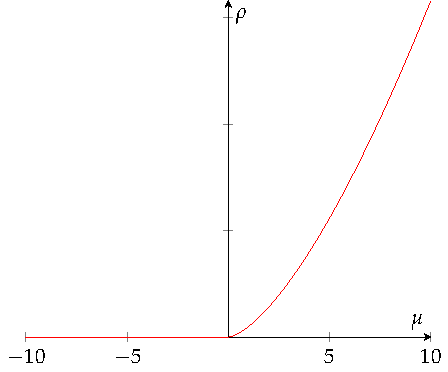
\includegraphics[]{Images/fig-rhomu.pdf}
    
    \caption{Plot of $\rho$ vs. $\mu$ (arbitrary units). $\rho$ is zero for $\mu \leq 0$ and $\rho \propto \mu^{3/2}$ for $\mu > 0$, signalling a phase transition in the system.}
    \label{fig-rhomu}
\end{figure}

The fact that $\rho \propto \mu^{3/2}$ is obtainable by realizing that $k_F \propto \rho^{1/3}$ (Eq. \eqref{eq-kF}) and $\mu = \e_F \propto k_F^2$ (Eqs. \eqref{eq-muef} and the definition of Fermi energy). Since $\phi \propto P \propto u$ (Eqs. \eqref{eq-phi} and \eqref{eq-P}), and $u \propto \rho^{5/3}$ (Eq. \eqref{eq-rho}), we find that the free energy $\phi$ is related to the chemical potential by $\phi \propto \mu^{5/2}$.

Since we have to take three derivatives of $\phi$ w.r.t. $\mu$ before we get a discontinuity (at $\mu = 0$), by the Ehrenfest classification of phase transitions, this is a third order phase transition. This discussion can also be taken as something that highlights the difference between Fermi gas and Fermi liquid behaviour; interactions change the properties of the system significantly.
\newpage
\section{Degenerate Bose Gas}
\subsection{Setting up the Boson Case}
Last time we discussed the Fermi gas, though we did not introduce any interactions. This is a starting point of doing condensed matter physics, nuclear physics (where the nucleus could be thought of as a small Fermi gas; though of course the interactions are strong in this case), neutron stars etc. When we add interactions, we get a Fermi liquid, where calculations become intractable; though we can apply computational methods in some cases. In a way, the strong interaction has been solved via a computer calculation; this is impressive as the models have been shown to work! Today, we instead discuss the degenerate Bose gas. We cover it as the second topic as it is more complex; due to Bose-Einstein condensation. We're stuck at zero temperature, and a gas of quantum-mechanical bosons at $T = 0$ (indeed, below some critical temperature $T_c$) forms a BE. If we're looking at particles without charge, we're looking at some kind of \emph{superfluid}. The noninteracting case is so ugly that we don't study it; we add a small interaction to make things more sensible, so the use of ``fluid'' is really correct, here.

We study a zero-temperature state of a box of bosons. If we ignore all interactions, the energy takes the form:
\begin{equation}
    \e = \frac{\hbar^2\v{k}^2}{2m}.
\end{equation}
Here, more than one particle can occupy the lowest energy state, so we might take our quantized field with the creation operator, and do something that looks nonsensical:
\begin{equation}
    (\alpha^\dag(0))^N\ket{0}
\end{equation}
Of course this looks crazy, as these particles with $\v{k} = \v{0}$ have infinite wavelength\dots so perhaps we should do something else, but what else is there? We could say that there is confinement within a box (of box $L$ with hard boundary conditions), but then the wavefunction would follow boundary conditions (in each direction).

\begin{figure}[htbp]
    \centering
    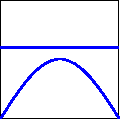
\includegraphics[]{Images/fig-bosonBC.pdf}

    \caption{Two possible views as the problem. We can constrain the bosons to a box of side length $L$ with hard boundaries, constraining the ground state wavefunction to look like $\sqrt{\frac{2}{L}}\sin(\frac{2\pi x}{L})$. Alteratively, we can assume our system is a finite patch out of infinite space, in which case the ground state wavefunctions are plane waves with infinite wavelength, i.e. constant in space.}
    \label{fig-bosonBC}
\end{figure}

In fact, the wavefunction and the energy would be quite sensitive to the boundary conditions. This is not something that we really want\footnote{as theorists in a QFT class, anyway; maybe not if you work at SBQMI down the street.}. We could do the opposite and remove the walls, and assume that our system is a finite patch within infinite space. Then a piece of the system should look fairly generic. But what happens then? The wavefunction would be constant over all space if $\v{k} = \v{0}$, so the probability of finding it anywhere in space is equal. So, our state is not something with a constant particle number. So at the outset, we can take this point of view that the particle number is not fixed; an approach that particle physicists and field theorists love. One could instead take a closed system and study it through this method, but there is not a consensus as to whether the two approaches are actually equivalent. But we will take the field theorists approach, here.

Motivated by this argument, we consider the state:
\begin{equation}
    \ket{\O} = \sum_{N=0}^\infty c_N\left(\alpha^\dag(\v{0})\right)^N \ket{0}.
\end{equation}
This is still not quite sensible; perhaps we can take something like:
\begin{equation}
    \alpha_f^\dag = \int d^3x f(\v{x})\alpha^{dag}(\v{k})
\end{equation}
for $f$ square integrable if we wanted to be a tad more rigorous, but let us not worry ourselves with this very much. How do we characterize such states? One thing we can notice is:
\begin{equation}
    \bra{\O}\psi(\v{x}, t)\ket{\O} \neq 0.
\end{equation}
The field operator annihilates a boson, but it will still have a nonzero overlap with the original vacuum state, so the overall expectation value will be nonzero (see HW2). Note that this is okay for bosons, but we would never see this for fermions. This is hugely degenerate if the bosons are non-interacting. 

\subsection{Coherent States}
Let us talk for a little about coherent states, which have the above expectation value property. At $t = 0$, we consider the field-operator commutation relations:
\begin{equation}
    [\psi(\v{x}), \psi^{\dag}(\v{y})] = \delta^{3}(\v{x} - \v{y})
\end{equation}
and:
\begin{equation}
    [\psi^\dag(\v{x}), \psi^{\dag}(\v{y})] =  [\psi(\v{x}), \psi(\v{y})] = 0.
\end{equation}
If we act the annhilation operator on the empty vacuum, we have:
\begin{equation}
    \psi(\v{x})\ket{0} = 0.
\end{equation}
We do not concern ourselves with the spin. Now, we consider the state:
\begin{equation}
    \ket{\eta} = e^{\int d^3x\left(\eta^*(\v{x})\psi(\v{x}) - \psi^\dag(\v{x})\eta(\v{x})\right)}\ket{0}
\end{equation}
where the operator in the exponential is anti-hermitian and so the overall operator is unitary. If we write the normal ordered version of the above, we obtain:
\begin{equation}
    \ket{\eta} = e^{-\int d^3x \eta^*(\v{x})\eta(\v{x})}e^{-\int d^3x \eta(\v{x})\psi^\dag(\v{x})}\ket{0}
\end{equation}
where we have got rid of the $\psi$ term by considering that this annhilates the vacuum state. We can write the action of the annihilation operator on the coherent state as:
\begin{equation}
    \psi(\v{x})\ket{\eta} = \eta(\v{x})\ket{\eta}.
\end{equation}
So that's a cool property! It's also a unitary transform of the vacuum state, so it is normalized:
\begin{equation}
    \braket{\eta}{\eta} = 1.
\end{equation}
So this is an example of the state where:
\begin{equation}
    \bra{\psi}\psi(\v{x})\ket{\eta} = \eta(\v{x}).
\end{equation}
This is an example of a ``good'' coherent state (as opposed to a bad one) and very often in physics we used bad ones. What could go wrong? For example, the integral $\int d^3x \eta^*(\v{x})\eta(\v{x})$ could diverge if $\eta(\v{x})$ is a constant. This often happens, actually (and we will proceed to work with this right now). The bad coherent state is ubiquotous; any interaction state of charges particles produces a ``coherent'' state of soft photons, but this is a bad coherent state (it has no overlap with any state which has a finite number of photons). Every QED interaction produces an infinite number of photons, which fly away undetected, but seem to be always there. So, we drop ``true/good'' coherent states for now, and work with bad ones; which will still give us sensible results.

\subsection{Landau's Argument for Superfluidity}
Note that in the textbook that there is a section which reviews Landau's famous argument about the quasiparticle spectrum and critical velocity of a superfluid. It uses Galilean symmetry, and so we don't cover it here (and the treatment of the book is so refined, that it is probably better to read it there). There is however the idea of a superfluid flowing through a pipe, without resistance, and so even if we introduce some interactions (between the particles, and with the pipe), it will flow through the pipe without any resistance. This is to some extent seen in the lab, and there is seen that if the superfluid goes too fast then the superfluid starts to feel resistance. Landau's argument goes as follows. For the energy to dissipate, there should be some excitations in the fluid. So, there should be some viscosity that creates a travelling wave/ripple (sometimes called quasiparticles) in the fluid. Let us say this is wavelike (everything is quantum mechanical here), with a wavenumber $\v{k}$ and frequency $\omega(\v{k})$. 

\begin{figure}[htbp]
    \centering
    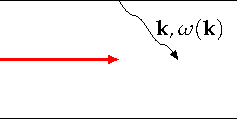
\includegraphics[]{Images/fig-superfluidpipe.pdf}

    \caption{In Landau's argument for superfluids, we consider a superfluid travelling in a pipe, and wavelike excitations/quasiparticles with wavenumber $\v{k}$ and frequency $\omega(\v{k})$.}
    \label{fig-superfluidpipe}
\end{figure}


He then argues that this should be energetically favourable if the velocity is larger than a critical velocity $v_c$:
\begin{equation}
    v_c = \min_\v{k} \frac{\omega(\v{k})}{\abs{\v{k}}}.
\end{equation}
The argument is beautiful in how it invokes Galilean relativity/symmetry (do read about it in your own time!) Note the stark difference from the free particle case; as then we would have $\omega(\v{k}) \propto \v{k}^2$ so $v_c = 0$, i.e. free particles are not superfluidic. What does work is if we have a sound wave, as then $\omega(\v{k}) = v_s\abs{\v{k}}$; here the critical velocity is the speed of sound.

So, the important goal for us; can we find this using our model? What do the elementary excitations look like?

A small aside; this argument doesn't really agree with experiments. $v_c$ as measured is smaller than what we would expect from Landau's argument. The explanation is that the dispersion relation $\omega(\v{k})$ as measured in experiment takes the form of the roton curve as seen in the below figure. Then $v_c$ is not the slope of the purple curve (as would be predicted theoretically) but instead is the slope of the red curve (less than the theoretically predicted value).

\begin{figure}[htbp]
    \centering
    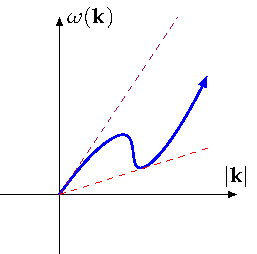
\includegraphics[]{Images/fig-rotoncurve.pdf}

    \caption{Plot of the experimental dispersion relation for superfluids (roton dispersion relation). From this we can see the reason for the experimental disagreement of the Landau argument for determining the critical velocity $v_c$ of superfluids, as the local minimum in the roton curve shifts the critical velocity to be the slope of the red curve, rather than the Landau theoretical prediction of the purple curve.}
    \label{fig-rotoncurve}
\end{figure}

\subsection{Introducing a Small Interaction to our QFT}
We introduce a weak repulsive interaction between the bosons that supresses the Bose-Einstein condensation. They will want to be far apart and run away from our system; so we add a chemical potential to balance this and draw them back in (so we end up with a finite density at the end). Let us write down a Hamiltonian\footnote{A remark: model building is often much easier than the actual toying with the (e.g. field) equations...} for this:
\begin{equation}
    H = \int d^3 x \left(\frac{\hbar^2}{2m}\nabla \psi^\dag(\v{x}) \cdot \nabla \psi(\v{x}) - \mu\psi^{\dag}(\v{x})\psi(\v{x}) + \frac{\lambda}{2}\psi^\dag(\v{x})\psi^{\dag}(\v{x})\psi_\v{x}\psi(\v{x})\right)
\end{equation}
where the last term is a ball-bearing potential, with $\lambda$ ``small'' (and positive; else the spectrum will not be bounded from below, as the energy from all the particles sitting on top of each other will be negative infinity). We also enforce the commutation relations:
\begin{equation}
    [\psi(\v{x}, t), \psi^{\dag}(\v{y}, t)] = \delta^3(\v{x} - \v{y}), \quad [\psi^\dag(\v{x}, t), \psi^{\dag}(\v{y}, t)] = [\psi(\v{x}, t), \psi(\v{y}, t)] = 0
\end{equation}
and also introduce the vacuum state $\ket{\O}$, which is the lowest-eigenvalue eigenstate of the (bounded-from-below) Hamiltonian. It is possible that the expectation value is nonvanishing, so let us anticipate this and introduce a function $\eta(\v{x})$:
\begin{equation}
    \bra{\O}\psi(\v{x}, t)\ket{\O} = \eta(\v{x}) \neq 0.
\end{equation}

How do we treat this possibility in a systematic way? One way would be to write:
\begin{equation}
    \psi(\v{x}, t) = \eta(\v{x}, t) + \tilde{\psi}(\v{x}, t)
\end{equation}
where $\eta$ is the classical part and $\tilde{\psi}$ is the quantum/non-classical part, i.e. which follows:
\begin{equation}
    \bra{\O}\tilde{\psi}(\v{x}, t)\ket{\O} = 0.
\end{equation}
So, there will be a classical part of the Hamiltonian where we forget about the $\tilde{\psi}$s, and in this term we would like $\eta$s which minimize the Hamiltonian. Then we can solve a classical field equation, check the extremum of the functional etc. We can argue that the $\eta$ that minimizes the Hamiltonian goes as:
\begin{equation}
    \eta \sim \frac{1}{\sqrt{\lambda}}.
\end{equation}
At very weak coupling, this classical piece is emphasized. We then might ask what the size of the quantum part is. Since $\psi$ needs to obey equal-time commutation relations, and $\eta$ drops out of these (as it is classical and drops out of the commutation relations), then since $\tilde{\psi}$ follows the commutation relations (where $\lambda$ shows up nowhere), this tells us that $\tilde{\psi}$ is of order unity:
\begin{equation}
    \tilde{\psi} \sim \lambda^0 = 1.
\end{equation}
If we make $\lambda$ small, we can then ignore anything but the classical $\eta$ term. We can consider an asymptotic expansion of $\eta$ (asymptotic as the first term is singular) and $\tilde{\psi}$, each of which have corrections which can be solved order by order. This is an arbitrarily good approach so long as $\lambda$ is arbitrary small and nonzero. Let us take it (next class!)

Another thing we might be interested in is the ``smoothest'' possible states, i.e. states that have some symmetry. A smooth surface has translation symmetry. We expect that the low-energy states of our theory here may be smooth. Suppose $\eta$ was a constant; then the most important part of our field is smooth. This is like going back to our condensate at the start of our lecture, where our wavefunctions were constant throughout all space. We then simply search for a constant which minimizes the Hamiltonian. The kinetic energy terms are zero if $\eta$ is a constant, and we can minimize the other terms to find:
\begin{equation}
    \eta = \sqrt{\frac{\mu}{\lambda}} \sim \frac{1}{\sqrt{\lambda}}.
\end{equation}
From our theory we can calculate the density:
\begin{equation}
    \rho \cong \frac{\mu}{\lambda}
\end{equation}
and the (grand canonical free) energy:
\begin{equation}
    \Phi = -\frac{\mu^2}{2\lambda} + \ldots = -\frac{\lambda}{2} \rho^2 + \ldots
\end{equation}
which is also equal to the negative of the pressure:
\begin{equation}
    P = -\Phi = \frac{\lambda}{2}\rho^2.
\end{equation}
So already this theory gives us a lot to work with, but we have yet to show that it is in fact a superfluid; this is something we will calculate and verify next class, by figuring out what $\omega(\v{k})$ is for our theory. 
\newpage
\section{Degenerate Bose Gas Continued}
\subsection{A Review of the Boson Gas Hamiltonian}
Recall the Hamiltonian we were working with in studying the Bose gas/liquid:
\begin{equation}
    H = \int d^3x\left(\frac{\hbar^2}{2m}\nabla \psi^\dag \cdot \nabla \psi - \mu \psi^\dag \psi + \frac{\lambda}{2}\psi^\dag\psi^\dag\psi\psi\right)
\end{equation}
where:
\begin{equation}
    \psi = \eta + \tilde{\psi}
\end{equation}
with $\eta$ is the classical part and $\tilde{\psi}$ the quantum part. We can interpret this as:
\begin{equation}
    \bra{\O}\tilde{\psi}\ket{\O} = 0.
\end{equation}
We noted that the classical part $\eta$ was very important in the weak-coupling limit, as $\eta \sim \frac{1}{\sqrt{\lambda}}$. Meanwhile, $\tilde{\psi}$ obeys commutation relations for which no $\lambda$ shows up, so $\tilde{\psi} \sim \lambda^0$. However, we expect that there are an infinite series of correction, so really:
\begin{equation}
    \psi = \eta + \tilde{\psi} + \delta \eta + \lambda \delta \tilde{\psi}
\end{equation}
Where $\delta \eta \sim \sqrt{\lambda}$. For small $\lambda$ (though this is not entirely a trivial statement; $\lambda$ has dimensions, so what it is small compared to?), it is meaningful to analyze the leading terms (i.e. a classical Hamiltonian). We can plug in $\eta$ to where the $\psi$s are in the Hamiltonian, and we get something that looks like a potential:
\begin{equation}
    V(\eta) = \mathcal{V}(-\mu\abs{\eta}^2 + \frac{\lambda}{2}\abs{\eta}^4)
\end{equation}
apologies for the confusing notation; $V$ on the left is the potential, $\mathcal{V}$ on the right is a volume. Minimizing $V$ (the potential) with respect to $\eta$, we find:
\begin{equation}
    \eta = \sqrt{\frac{\mu}{\lambda}}.
\end{equation}
There is something funny with this identification; $V(\eta)$ depends only on the norm of $\eta$, but in the expression for $\eta$ we have chosen it to be real. From a minimization perspective:
\begin{equation}
    \eta = \sqrt{\frac{\mu}{\lambda}}e^{i\theta}
\end{equation}
are valid minima for all $\theta \in \RR$. So the minimum is not unique. However, we can proceed by just choosing an angle of our choice, and it will not matter. Why is this the case? 


\subsection{A Brief Foray Into Spontaneous Symmetry Breaking}
Looking at the Hamiltonian, we notice that there is a symmetry; namely, the Hamiltonian is unchanged by the introduction of some phase $\psi \mapsto \psi e^{i\theta}$. So, this tells us that what we choose for the phase of $\eta$ should not matter. 

\begin{figure}[htbp]
    \centering
    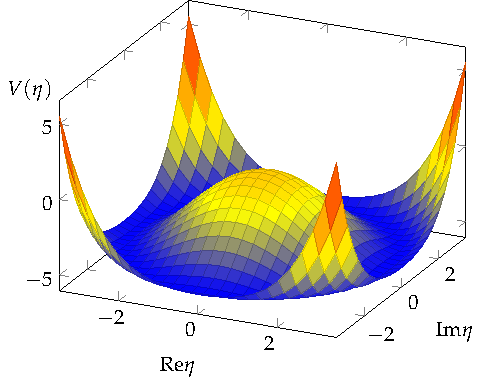
\includegraphics[]{Images/fig-etapotential.pdf}
    \caption{3D plot of the potential $V$ as a function of $\eta$. We take $\mathcal{V} = 1, \mu = 1, \lambda = 1/10$.The blue ring corresponds to $\eta = \sqrt{\frac{\mu}{\lambda}}e^{i\theta}$ which minimizes the potential, which is radially symmetric.}
    \label{fig-etapotential}
\end{figure}

The idea is that the potential is completely symmetric under rotation, but the solution is not. This is something known as spontaneous symmetry breaking. Classical analogy: which way does chalk fall when one lets go of it from the top position. A priori, there is a symmetry; there is no preference to how it falls. But when we actually do the experiment, it falls somewhere as we perturb it somehow when releasing (breaking the symmetry) or an air molecule bounces off of it and causes it to fall. Quantum mechanically, the chalk is described by the rigid rotator Hamiltonian:
\begin{equation}
    H = \frac{I}{2}\dot{\theta}^2
\end{equation}
If I look at the eigenfunctions, we have:
\begin{equation}
    \psi(\theta) = e^{in\theta}
\end{equation}
The ground state is a superposition of all of these angles, which averages out to zero. But this is clearly not the right state; it is in some orientation and it is frozen there. The idea is that the chalk pointing at some angle is actually an excited state; we have something like:
\begin{equation}
    \psi(\theta) = \sum_n e^{in(\theta - \theta_c)}
\end{equation}
and it relaxes towards the ground state given sufficient time; however this time depends on the moment of inertia, which here it is very large. If the chalk was small enough, then we would see it undergo this relaxation; since it is macroscopic, the relaxation time is very large. 

Why this chalk discussion? This is to say that why the quantum mechanical description of the chalk may be correct, it is really not particularly reasonable; it makes more sense to treat this classically.  So, returning back to the idea of spontaneous symmetry breaking. This is a ubiqitous phenomenon (in condensed matter, particle physics, etc.). For example, consider ferromagnetism. The true ground state of a ferromagnetic is some superposition, but if we look at it, it will not decay to the ground state during the lifetime of the universe. So, we can just think about this classically.

Having now chosen a solution, we can't see the symmetry of the whole potential anymore; the fluctuations (as obtained by calculating the higher order terms) cannot ``see'' the whole energy landscape (one can think that the ``moment of inertia'' is so large that it cannot explore the entire ring of minima).

A takeaway from all of this; spontaneous symmetry-breaking is a phenomena we often see when classical effects dominate over quantum ones.

\subsection{Solving the System}
So, we've solved for the leading term of the expansion of $\psi$! Since it's dominant, we could just calculate the internal energy, or the grand canonical free energy from what we have so far. We can find the GC free energy to be:
\begin{equation}
    \varphi = -\frac{\lambda}{2}\rho^2 = -P.
\end{equation}
We can find corrections to this by calculating the contributions from the higher order terms (these corrections should be small, if our asymptotic expansion is actually reasonable). In particular, here this expansion works at low density.

Next, we can plug $\psi = \eta + \tilde{\psi}$ into the field equation (see HW2) or the Hamiltonian (which we do now), and see what we get out. We find:
\begin{equation}
    H' = -\frac{\lambda}{2}\rho^2 V + \int d^3x \left(\frac{\hbar^2}{2m}\nabla \tilde{\psi}^\dag \cdot \nabla \tilde{\psi} + \mu \tilde{\psi}^\dag \tilde{\psi} + \frac{\mu}{2} \tilde{\psi} \tilde{\psi} + \frac{\mu}{2}\tilde{\psi}^\dag \tilde{\psi}^\dag\right) + \O(\lambda)
\end{equation}
Now the Hamiltonian does not look normal in the $\tilde{\psi}$ and $\tilde{\psi}^\dag$s anymore; this is due to the broken symmetry. We can also plug in our expansion into the commutation relations:
\begin{equation}
    [\tilde{\psi}(\v{x}, t), \tilde{\psi}^\dag(\v{y}, t)] = \delta^3(\v{x} - \v{y})
\end{equation}
Let us comment on the $\O(\lambda)$ corrections; we first have that:
\begin{equation}
    -\frac{\lambda}{2}\rho^2V = -\frac{\mu^2}{2\lambda}V
\end{equation}
So this is indeed the leading term for small $\lambda$. The integral term is of order $\lambda^0 = 1$. Then the corrections are of order $\lambda$, so we can control these by taking small $\lambda$.

For large derivatives, the kinetic energy terms dominate, but for smaller derivatives the other terms in the integral become important. 

By plugging things back in, we get a linear field equation for $\tilde{\psi}$ (The Bogolibov-de-Gennes equation); see HW2. But let us attack this Hamiltonian directly:
\begin{equation}
    \psi(\v{x}, 0) = \int \frac{d^3k}{(2\pi)^{3/2}}e^{i\v{k} \cdot \v{x}}\alpha(\v{k})
\end{equation}
this is really just a change of basis in function space; the whole integral is like a unitary matrix that rotates the basis. Let us go to the $\alpha$s; why? Because the Hamiltonian is translation invariant, we would suspect that the momentum would be an important quantity, and $\v{k}$ is closely related to momentum, so it is good to analyze. The Hamiltonian reads:
\begin{equation}
    H = -\frac{\mu^2}{2\lambda}V + \int d^3k \left(\frac{\hbar^2k^2}{2m}\alpha^\dag(\v{k})\alpha(\v{k}) + \mu \alpha^\dag(\v{k})\alpha(\v{k}) + \frac{\mu}{2}\alpha(-\v{k})\alpha(\v{k}) + \frac{\mu}{2}\alpha^\dag(\v{k})\alpha^{\dag}(-\v{k})\right)
\end{equation}
From going to $k$-space, we have a separate Hamiltonian for each value of $\v{k}$, and the first term ($\alpha^\dag(\v{k})\alpha(\v{k})$) is diagonalized. However, it is still not clear what the eigenvalues of the elementary excitations are. We need to diagonalize this Hamiltonian; let us try this. First we note that the Hamiltonian is of quadratic form, so we should be able to diagonalize it. We let:
\begin{equation}\label{eq-bogoliubov}
    \begin{split}
        \alpha(\v{k}) &= \cosh\theta(\v{k})a(\v{k}) - \sinh\theta(\v{k})a^{\dag}(-\v{k})
        \\ \alpha^\dag(\v{k}) &= \cosh\theta(\v{k})a^\dag(\v{k}) - \sinh\theta(\v{k})a(-\v{k})
    \end{split}
\end{equation}
Wait, where do the hyperbolic functions come from? We know that the $\alpha$s follow the commutation relations:
\begin{equation}
    [\alpha(\v{k}), \alpha^\dag(\v{l})] = \delta^3(\v{k} - \v{l})
\end{equation}
so we want the $a$s to do the same:
\begin{equation}
    [a(\v{k}), a^\dag(\v{l})] = \delta^3(\v{k} - \v{l})
\end{equation}
I don't have a lot of freedom in the coefficients if I want the commutation relations to hold; the hyperbolic functions come out of this.

Eqs. \eqref{eq-bogoliubov} is known as a Bogoliubov transformation. We can plug this into the Hamiltonian and get an even more complicated expression with $\sin\theta(\v{k})$s and $a$s, and we can adjust $\theta(\v{k})$ until we get something proportional to $a^\dag(\v{k})a(\v{k})$. When we do so, we end up with:
\begin{equation}
    H = -\frac{\mu^2}{2\lambda}V + \int d^3k E(\v{k})a^\dag(\v{k})a(\v{k}) + E_0
\end{equation}
where the constant at the end comes from the corrections from interchanging the order of operators (as a consistency check: this constant should be small compared to the leading order constant). It is a kind of zero-point energy. In order for the above to hold, we find the constraint that:
\begin{equation}
    \tanh2\theta(\v{k}) = \frac{\mu}{\frac{\hbar^2\v{k}^2}{2m} + \mu}
\end{equation}
and $E(\v{k})$ follows:
\begin{equation}
    E(\v{k}) = \sqrt{\left(\frac{\hbar^2\v{k}^2}{2m} + \mu\right)^2 - \mu^2}
\end{equation}
so we obtain a dispersion relation for $\v{k}$! The cool thing is we can now use this dispersion relation combined with the Landau result to get a testable prediction of the critical velocity for superfluids. For small $\v{k}$, the above reduces to:
\begin{equation}
    E(\v{k}) \approx \sqrt{\frac{\hbar^2}{2m}\mu}\abs{\v{k}}
\end{equation}
So the Landau criterion would tell us that:
\begin{equation}
    v_c = \sqrt{\frac{\hbar^2}{2m}\mu}.
\end{equation}
This turns out to be wrong most of the time, as superfluids are in general not weakly interacting. But, when an experimental group created a weakly-interacting Bose-Einstein condensate, they were able to indeed verify that the above expression holds!

This concludes our discussion; HW2 attacks the same problem from the perspective of the equations of motion.

\subsection{A Small Teaser for Next Lecture}
We've developed our QFT, rewrote many-particle QM as a QFT, and studied some simple (but useful!) examples (such as the Fermi gas\footnote{Quite a useful ``first-order'' approximation for metals.} and superfluids). Now, we go into developing the ideas of QFT a little further. One might wonder why we need something else; this is because this ``something else'' gives us great power and a nicer way to study field theories when we have to do perturbation theory. It may be an unexpected step, but we will temporarily regress from doing QFT to doing classical field theory. We will consider the \emph{action principle}. We will consider some classical field $\psi_\sigma(\v{x}, t)$ (bosons only; anti-commuting fermions would not be pure functions, but would instead be operators belonging to an algebra...). We will then ask if we can derive our field equation from a variational principle and an action. Of course the answer is yes (else we wouldn't bring it up), and we can even write down the Lagrangian density and the action which will yield our classical field equation. The action is:
\begin{equation}
    S = \int dt d^3x \L
\end{equation}
where the Lagrangian density is:
\begin{equation}
    \L = i\hbar \psi^{\dag\sigma}\dpd{}{t}\psi_\sigma - \frac{\hbar^2}{2m}\nabla \psi^{\dag\sigma} \cdot \nabla \psi_\sigma + \mu \psi^{\dag\sigma}\psi_\sigma - \frac{\lambda}{2}\left(\psi^{\dag\sigma}\psi_\sigma\right)^2.
\end{equation}
However, we have lost something: our quantum field equation had a particular ordering of the $\psi$ and $\psi^\dag$s in the interaction part. We have to recover this somehow. This could be a small or large problem; for us it is small because we know how it has to look like ahead of time. But, something like the ordering problem in treating Einstein's gravity is not resolved. In general, this is something one needs to solve case-by-case.

What then, do we gain? The Lagrangian encodes the commutator as well as the field equation. One can encode the first term as:
\begin{equation}
    \left(i\hbar \psi^{\dag\sigma}\right)\left(\dpd{}{t}\psi_\sigma\right) = P\dot{Q}
\end{equation}
and note the connection with the Hamiltonian:
\begin{equation}
    L = P\dot{Q} - H(P, Q).
\end{equation}
One can consider the Poisson bracket:
\begin{equation}
    \{\psi_\sigma(\v{x}, t), i\hbar\psi^{\dag\rho}(\v{y}, t)\} = \delta_\sigma^\rho\delta^3(\v{x} - \v{y})
\end{equation}
and when quantizing one adds an $i\hbar$ and replaces the Poisson bracket with a commutator. So there is that benefit of less writing. We also gain the analysis of symmetries and conserved quantities that we know from classical field theory, which we can lift to the QFT (for example, conservation of energy, momentum).

This is not just a construct; we will learn how to use functional integrals, and the (classical) action plays a very large role there (we integrate over it). It will stay with us for a long time.
\newpage
\section{The Action Principle}
We revert a little bit back into classical field theory. Technically, the field equation and the commutation relations we have constructed define our QFT, and give us all the information we need. So changing the formalism needs some justification; that justification is that classical field theory has a lot of structure, we can lift back into QFT to learn more about QFT. This logic is fairly obscure in most textbooks, but we will explore it a bit deeper. We will find the classical to quantum transition to be relatively straightforwards. For generic quantum theories, this is not the case, but quantum field theories tend to be simple as far as mechanical things go. This is not just because we like simple things, but because the internal consistency of quantum field theories doesn't let them be extremely complicated.

\subsection{The Action \& Lagrangians}
The action is defined as the following integral over spacetime:
\begin{equation}
    S = \int d^3x dt \L = S[\psi, \psi^\dag]
\end{equation}
where $\L$ is the Lagrangian density. It is a functional; it maps functions $\psi, \psi^\dag$ onto a number $S$. We consider the Lagrangian density:
\begin{equation}
    \L = \frac{i\hbar}{2}\psi^{\dag\sigma}\dpd{\psi_\sigma}{t} - \frac{i\hbar}{2}\dpd{\psi^{\dag\sigma}}{t}\psi_\sigma - \frac{\hbar^2}{2m}\nabla \psi^{\dag\sigma} \cdot \nabla \psi_\sigma + \mu \psi^{\dag\sigma}\psi_\sigma - \frac{\lambda}{2}(\psi^{\dag\sigma}\psi_\sigma)^2.
\end{equation}
this is the Lagrangian that would recover our non-relativistic quantum field theory (we just conjured this up, with some guidelines; namely that it reproduces the field equation that we want. The field equation is the primitive here, and the Lagrangian we reverse engineer\footnote{But note that once we start to familiarize ourselves with Lagrangians, we will find it easier to write down a Lagrangian and derive the field equations etc. from there. It is a slightly shorter presentation of all of the data encoded in the field equation and commutation relations.}). From this Lagrangian we can not only recover the field equation but also the commutator.

Note that for free field theories, we will in general only consider Lagrangians that are quadratic in the fields; this allows for the equations of motion to be linear. For interacting field theories we may have higher order terms. 

Now, if we consider the relation of the Lagrangian to the Hamiltonian:
\begin{equation}
    \L = P\dot{Q} - H(P, Q) =  i\hbar\psi^{\dag\sigma}\dpd{\psi_\sigma}{t} - \ldots
\end{equation}
We can identify $Q$ with $\psi_{\sigma}(\v{x}, t)$ and $P$ with $i\hbar \psi^{\dag\rho}(\v{x}, t)$. The Poisson bracket then gives us:
\begin{equation}
    \{\psi_{\sigma}(\v{x}, t), i\hbar\psi^{\dag\rho}(\v{x}, t)\} = \delta_{\sigma}^\rho \delta^3(\v{x} - \v{y})
\end{equation}
So if we then go from classical to quantum by changing the Poisson brackets to commutators and introducing a factor if $i\hbar$, we have:
\begin{equation}
    [\psi_{\sigma}(\v{x}, t), i\hbar\psi^{\dag\rho}(\v{x}, t)] = i\hbar\delta_{\sigma}^\rho \delta^3(\v{x} - \v{y}) \implies [\psi_{\sigma}(\v{x}, t), \psi^{\dag\rho}(\v{x}, t)] = \delta_{\sigma}^\rho \delta^3(\v{x} - \v{y}).
\end{equation}
Next, how do we get the field equation? The action principle states that the action functional, considered as a mapping of classical fields obeying the appropriate boundary conditions to the real numbers, is stationary when it is evaluated on the field configurations which obey the classical equations of motion, that is, the classical field equation. So, the Lagrangian encodes the field equation, and we can suss it out through some calculus of variations/functional calculus.

\subsection{Deriving the Euler-Lagrange Equations}
We write down a formal mathematical criteria for what this means. $\psi, \psi^\dag$ are a ``stationary point'' (of course one remembers these are actually functions) when:
\begin{equation}
    S[\psi + \delta \psi, \psi^\dag + \delta \psi^\dag] = S[\psi, \psi^\dag] + O((\delta\psi)^2, (\delta \psi^{\dag})^{2}, \delta\psi\delta\psi^{\dag}) = S[\psi, \psi^\dag] + \delta S
\end{equation}
One might ask what a ``nearby point'' in function space actually is (i.e. what does $\delta \psi$ mean?); we avoid this discussion as our applications tend to be simple. 

We can now define the variation of the action as follows (by considering the variation of the Lagrangian, treating it as a function of $\psi_\sigma, \psi^{\dag\sigma}$ and its spatial/time derivatives):

\begin{equation}
    \begin{split}
        \delta S &= \int dt d^3 x \delta \L
        \\ &=\int dt d^3x \left[ \delta \psi_\sigma(\v{x}, t) \dpd{\L}{\psi_\sigma(\v{x}, t)} + \delta \dot{\psi}_\sigma(\v{x}, t) \dpd{\L}{\dot{\psi}_\sigma(\v{x}, t)} + \delta \nabla \psi_\sigma(\v{x}, t)\dpd{\L}{\nabla \psi_\sigma(\v{x}, t)} + (\psi_\sigma \iff \psi^{\dag\sigma})\right]
    \end{split}
\end{equation}
where $(\psi_\sigma \iff \psi^{\dag\sigma})$ denotes we have all the same terms, replacing the $\psi$s with their Hermitian conjugate. We can then consider that:
\begin{equation}
    \delta(\nabla \psi_\sigma(\v{x}, t)) = \nabla(\delta \psi_\sigma(\v{x}, t))
\end{equation}
i.e. the variation of the derivative is the derivative of the variation, and the same with the time derivatives:
\begin{equation}
    \delta(\dpd{}{t}\psi_\sigma(\v{x}, t)) = \dpd{}{t}(\delta\psi_\sigma(\v{x}, t))
\end{equation}
We can then rewrite the variation of the action as:
\begin{equation}
    \delta S = \int dtd^3x \left[\delta \psi_\sigma(\v{x}, t)\left(\dpd{\L}{\psi_\sigma} - \dpd{}{t}\dpd{\L}{\dot{\psi}_\sigma} - \nabla \cdot \dpd{\L}{\nabla \psi_\sigma}\right) + \dpd{}{t}\left(\delta \psi_\sigma\dpd{\L}{\dot{\psi}_\sigma}\right) + \nabla \cdot \left(\delta \psi_\sigma\dpd{\L}{\nabla \psi_\sigma}\right) + (\psi_\sigma \iff \psi^{\dag\sigma})\right]
\end{equation}
We look at the second and third terms in the above integral. It is a four-divergence, so Gauss’s theorem allows us to rewrite its spacetime volume integral as a surface integral at the boundaries of space and time.
While we don't concern ourselves with the details of Dirchlet vs. Neumann boundary conditions, we assume that there is some BC which makes the surface terms vanish:
\begin{equation}
    \dpd{}{t}\left(\delta \psi_\sigma\dpd{\L}{\dot{\psi}_\sigma}\right) = \nabla \cdot \left(\delta \psi_\sigma\dpd{\L}{\dot{\psi}_\sigma}\right) = 0
\end{equation}
So, if we set $\delta S = 0$, this tells us that the first quantity in brackets must vanish if $\delta \psi_\sigma(\v{x}, t)$ has an arbitrary profile; we thus get the Euler-Lagrange equations:
\begin{equation}
    \begin{split}
        &\dpd{\L}{\psi_\sigma(\v{x}, t)} - \dpd{}{t}\dpd{\L}{\dot{\psi}_\sigma(\v{x}, t)} - \nabla \cdot \dpd{\L}{\nabla \psi_\sigma(\v{x}, t)} = 0
        \\ &\dpd{\L}{\psi^{\dag\sigma}(\v{x}, t)} - \dpd{}{t}\dpd{\L}{\dot{\psi}^{\dag\sigma}(\v{x}, t)} - \nabla \cdot \dpd{\L}{\nabla \psi^{\dag\sigma}(\v{x}, t)} = 0
    \end{split}
\end{equation}
In ``normal'' classical mechanics, we don't have the third term, but in our case we do have a spatial dependence. A note: one can see that this already lifts nicely to relativistic physics. Another note: potentials can cause some complication, here.

We can get the field equations from the EL-equations, and we have already derived the commutator. There is still the issue of operator ordering. In this non-relativistic theory, it is the only place that we see it. But in general this is something one must keep in mind.

Other than recovering what we previously had, we actually get more! This is in the context of classical field theory, and it has to do with symmetries. 

\subsection{Symmetry and Noether's Theorem}
The kinds of symmetry we are interested in are where there is some infinitesimal transformation (i.e. continuous symmetries). For example a rotation, or translation (an example of one without an infinitesimal transformation would be parity).

We take our field variable, and we transform it to some other field variable:
\begin{equation}
    \begin{split}
        &\psi_\sigma(\v{x}, t) \to \tilde{\psi}_\sigma(\v{x}, t) = \psi_\sigma(\v{x}, t) + \delta\psi_\sigma(\v{x}, t)
        \\ &\psi^{\dag\sigma}(\v{x}, t) \to \tilde{\psi}^{\dag\sigma}(\v{x}, t) = \psi^{\dag\sigma}(\v{x}, t) + \delta\psi^{\dag\sigma}(\v{x}, t)
    \end{split}
\end{equation}
Where we can take the transformation to be linear as we consider infinitesimal transformations (higher orders negligeble). We can now consider how the Lagrangian transforms under this. We say that this is a \emph{symmetry} (this is our definition) if $\delta \L$ can be organized (algebraically; without looking at the equations of motion) in the following way:
\begin{equation}
    \delta \L = \dpd{}{t}R(\v{x}, t) + \nabla \cdot \v{J}(\v{x}, t)
\end{equation}
If things drop off at infinity, then this is a way of saying that the action doesn't change. Some textbooks require the Lagrangian to be invariant; we do not enforce this constraint here.

Now, having defined a symmetry, we can invoke the equations of motion and see what more we can learn. If we assume that the equation of motion is obeyed, then we have that:
\begin{equation}
    \delta \L = \dpd{}{t}\left(\delta \psi_\sigma\dpd{\L}{\dot{\psi}_\sigma}\right) + \nabla \cdot \left(\delta \psi_\sigma\dpd{\L}{\nabla\psi_\sigma}\right) + (\psi_\sigma \iff \psi^{\dag\sigma})
\end{equation}
So we now have two equations for $\delta \L$; their difference should then be zero:
\begin{equation}
    \begin{split}
        &0=\frac{\partial}{\partial t}\left[\delta \psi_\sigma(\vec{x}, t) \dpd{\L}{\dot{\psi}_\sigma(\v{x}, t)} + \delta \psi^{\dag\sigma}(\vec{x}, t) \dpd{\L}{\dot{\psi}^{\dag\sigma}(\v{x}, t)} - R(\v{x}, t)\right] 
        \\ &+ \nabla \cdot \left[\delta \psi_\sigma(\vec{x}, t) \dpd{\L}{\nabla\psi_\sigma(\v{x}, t)} + \delta \psi^{\dag\sigma}(\vec{x}, t) \dpd{\L}{\nabla\psi^{\dag\sigma}(\v{x}, t)} - \v{J}(\v{x}, t)\right]
        \\ &\implies \dpd{}{t}\mathcal{R}(\v{x}, t) + \nabla \cdot \gv{\mathcal{J}}(\v{x}, t) = 0
    \end{split}
\end{equation}
in other words, we have a conservation law! The symmetry implies a conservation law, and a systematic way of finding the conserved quantity; this is the power of the Lagrangian. This is \emph{Noether's Theorem}. $\mathcal{R}$ is the Noether charge density and $\gv{\mathcal{J}}$ is the Noether current density. If we now integrate, we find:
\begin{equation}
    \dpd{}{t}\int_\Omega d^3 x \mathcal{R}(\v{x}, t) = -\oiint_{\partial \Omega} d\v{n} \cdot \gv{\mathcal{J}}(\v{x}, t)
\end{equation}
In otehr words the change in the Noether charge is just the Noether current that flows across the boundary. We can now lift this to quantum field theories, where we will find great use of these results. Next time we will explore various examples of symmetries, and see what Noether's theorem has to say about their associated conserved quantities.
\newpage
\section{Symmetries \& Noether's Theorem}

Last time we reverted from quantum to classical field theory. We did this to cast our field theory in terms of a Lagrangian and equations of motion derived from them; this had the benefit of allowing us to use Noether's theorem, which tells us about conserved quantities and how to determine what they are. We can then lift these equations of motion back into our QFT, showing that operators in our QFT are also conserved. There are two problems in the way; the first is operator ordering issues, and the second is that products of operators at the same point requires some mathematical definition, which can be add odds with the conservation law! This can actually lead to interesting physics though; in particle physics these are known as anomalies, e.g. in pion decay. The miracle is that this fooling around with operators leads to effects that are experimentally observable. Abstract and seemingly ad-hoc mathematics have physical impact!

But we won't go there (at least for now); we will first study some examples of symmetries and Noether's Theorem. We need an example theory before we find symmetries of said theory; let's write down our favourite one:
\begin{equation}
    \L = \frac{i\hbar}{2}\psi^\dag \dpd{\psi}{t} - \frac{i\hbar}{2}\dpd{\psi^\dag}{t}\psi - \frac{\hbar^2}{2m}\nabla \psi^\dag \cdot \nabla \psi - \frac{\lambda}{2}(\psi^\dag \psi)^2
\end{equation}
where we have omitted the $\v{x}$s and spin indices for brevity. The symmetrized time derivative part ensures that it is real. We also don't include chemical potential for now. But note it is useful for operator ordering issues; changing the order of terms generates extra constants, and the chemical potential can be used to absorb these ambiguities.

\subsection{Phase Symmetry}
One transformation that leaves $\L$ invariant is to multiply $\psi$ by some phase (we can see this as each $\psi$ is paired with $\psi^\dag$). So we can write down an infinitesmal version of this transformation:
\begin{equation}
    \begin{split}
        \delta \psi &= i\theta\psi
        \\ \delta \psi^\dag &= -i\theta \psi^\dag
    \end{split}
\end{equation}
we can test that this is indeed a symmetry by seeing if we can write the Lagrangian as a total derivative under it; but it is even easier than that here; just plugging it in, to linear order we see that:
\begin{equation}
    \delta \L = 0
\end{equation}
i.e. the Lagrangian density doesn't change at all. We call this \emph{phase symmetry}. Going back to our expression from last class of the Noether current and Noether charge density, we have:
\begin{equation}
    \mathcal{R}(\v{x}, t) = \delta \psi \dpd{\L}{\dot{\psi}} + \delta \psi^\dag \dpd{\L}{\dot{\psi}} = \hbar \theta \psi^\dag \psi = 0
\end{equation} 
We see what we would have called the number operator in the QFT popping out on the RHS; in other words, the particle number is a conserved Noether charge of some kind. We can also write:
\begin{equation}
    \gv{\mathcal{J}} = \delta \psi \dpd{\L}{\nabla \psi} + \delta \psi^\dag \dpd{\L}{(\nabla \psi^\dag)} = 0.
\end{equation}
so we also get information about the flux of the particle number. We have the following expression for the particle current:
\begin{equation}
    \gv{\mathcal{J}} = i\theta\frac{\hbar^2}{2m}(\nabla \psi^\dag)\psi - \frac{i\theta\hbar^2}{2m}(\psi^\dag \nabla \psi)
\end{equation}
If this follows a continuity equation, then so will the above multiplied by a constant; so we learn:
\begin{equation}
    \dpd{}{t}(\psi^\dag\psi) + \nabla \cdot \left(\frac{i\hbar}{2m}\nabla \psi^\dag \psi - \frac{i\hbar}{2m}\psi^\dag \nabla \psi\right) = 0
\end{equation}
We can define the density:
\begin{equation}
    \rho(\v{x}, t) = \psi^{\dag\sigma}(\v{x}, t)\psi_\sigma(\v{x}, t)
\end{equation}
and the current:
\begin{equation}
    \v{J}(\v{x}, t) = -\frac{i\hbar}{2m}\left(\psi^{\dag\sigma}(\v{x}, t)\nabla \psi_\sigma(\v{x}, t) - \nabla \psi^{\dag\sigma}(\v{x}, t)\psi_\sigma(\v{x}, t)\right)
\end{equation}
So this is our first example of a conservation law (note: this follows from Noether's Theorem, which we proved last time!); phase symmetry leads to the conservation of particle number. Note that the above example is operator ordering ambiguous, so it should lift nicely to QFT; it tells us if our theory has a phase symmetry, then:
\begin{equation}
    \dpd{}{t}\mathcal{N} = \dpd{}{t}\int d^3x \rho(\v{x}, t) = 0
\end{equation}
We knew this already for specific examples, but now we have a more general argument; we know it to be true for any theory with a phase symmetry. Now, what else can we do?

\subsection{Translational Symmetry and the Stress Tensor}
We would expect that our theory is translation invariant in both time and in space, as there are now explicit $t$s or $x$s anywhere. These should lead to conservation of energy and momentum, respectively. A time translation would be:
\begin{equation}
    \psi(\v{x}, t) \to \psi(\v{x}, t + \e) \approx \psi(\v{x}, t) + \e\dpd{}{t}\psi(\v{x}, t)
\end{equation}
and a space translation would be:
\begin{equation}
    \psi(\v{x}, t) \to \psi(\v{x} + \gv{\e}, t) \approx \psi(\v{x}, t) + \e\nabla \psi(\v{x}, t)
\end{equation}
So we could then write:
\begin{equation}
    \begin{split}
        \delta \psi &= (\e\dpd{}{t} + \gv{\e} \cdot \nabla)\psi
        \\ \delta \psi^\dag &= (\e\dpd{}{t} + \gv{\e} \cdot \nabla)\psi^\dag
    \end{split}
\end{equation}
since $\L$ does not depend on $t$ or $\v{x}$, if we make the above infinitesimal transformations, the change in the Lagrangian would look like:
\begin{equation}
    \delta \L = (\e\dpd{}{t} + \gv{\e} \cdot \nabla)\L = \dpd{}{t}(\e\v{L}) + \nabla \cdot (\gv{\e}\L)
\end{equation}
so it satisfies a symmetry criterion, and therefore there is a conserved charge; in fact there are four, one for each component of $\e$ (like a conserved four-vector)! Then there are 3 conserved currents for each of these. The best way to write this is as a 4x4 matrix; let's set this up.
\begin{equation}
    \mathcal{R}(\v{x}, t) = \left(\e\dpd{}{t} + \gv{\e} \cdot \nabla\right) \psi \dpd{\L}{\dot{\psi}} + \left(\e\dpd{}{t} + \gv{\e} \cdot \nabla\right)\psi^\dag \dpd{\L}{(\nabla \psi^\dag)} - (\e\L)
\end{equation}
and there are one of these for each of the four $\e$s. The current densities are analogous:
\begin{equation}
    \gv{\mathcal{J}}(\v{x}, t) = \left(\e\dpd{}{t} + \gv{\e}\cdot\nabla\right)\psi\dpd{\L}{(\nabla \psi)} + \left(\e\dpd{}{t} + \gv{\e}\cdot\nabla\right)\psi^\dag \dpd{\L}{(\nabla \psi^\dag)} - \gv{\e}\L
\end{equation}
we now write this as a matrix, known as the energy-momentum (stress) tensor:
\begin{equation}
    \m{\mathbb{T}^{tt} &\mathbb{T}^{ta} \\ \mathbb{T}^{bt} & \mathbb{T}^{ba}}
\end{equation}
where the first row is the time row, and the latter three are the space rows (and analogously for the columns). $a, b$ range over $xyz$. The conservation laws for each of these quantities looks like:
\begin{equation}
    \dpd{}{t}\mathbb{T}^{tt} + \dpd{}{(x^b)}\mathbb{T}^{bt} = 0
\end{equation}
\begin{equation}
    \dpd{}{t}\mathbb{T}^{ta} + \dpd{}{(x^b)}\mathbb{T}^{ba} = 0.
\end{equation}
where the derivatives act on the first indices, and the second label points to the symmetry we are talking about. We can then read off the components of the stress tensor:
\begin{equation}
    \mathbb{T}^{tt} = \dpd{\psi}{t}\dpd{\L}{\dot{\psi}} + \dpd{\psi^\dag}{(\dot{\psi}^\dag)}\dpd{\L}{(\dot{\psi}^\dag)} - \L = \H = \frac{\hbar^2}{2m}\nabla \psi^\dag \cdot \nabla \psi + \frac{\lambda}{2}(\psi^\dag\psi)^2
\end{equation}
we recognize this as the Hamiltonian density. So what is conserved here is the integral of this over space, i.e. the total energy! The other components are:
\begin{equation}
    \mathbb{T}^{ta} = \dpd{\psi}{(x^a)}\dpd{\L}{\dot{\psi}} + \dpd{\psi^\dag}{(x^a)}\dpd{\L}{(\dot{\psi}^\dag)}
\end{equation}
note we've stripped off the $\e$ as it is just an overall factor. We also don't include the $-\L$ term in the above. This we can recognize as the momentum density, whose integral is the spatial momentum; which is conserved. You can get the three space components by varying $a = x,y,z$, and each of these are conserved.

Note that writing the stress tensor does not do anything except save us some writing. In conclusion, we have the conserved quantities:
\begin{equation}
    U = \int d^3 x \mathbb{T}^{tt}(\v{x}, t)
\end{equation}
\begin{equation}
    P^a = \int d^3x \mathbb{T}^{ta}(\v{x}, t)
\end{equation}
Does this lift to the quantum field theory? The momentum is easy because it turns out to be quadratic. Just looking at $\mathbb{T}^{ta}$, we can see that it only depends on the first terms of the Hamiltonian; it doesn't care about the interactions. Any interaction that has space translation invariance will have the same expression for the momentum density and the moementum itself. Moreover, it is the same as the number operator case where there is no operator ordering ambiguity.

However, there is an ambiguity for the $\mathbb{T}^{tt}/$energy term. This is more or less an ad-hoc procedure where we guess ordering until it works. Luckily we don't encounter this issue very much, and in this case we already know what the ordering is. So we know how to deal with it already.

\subsection{Galilean Relativity}
A teaser for next day: translation symmetry in space and time give us a tensor. There are some more symmetries, though; in a sense symmetries of a generic theory (symmetries that lots of theories share), which go in the direction of relativity. Even in non-relativistic physics, there are concepts of relativity. One example is Galilean symmetry/relativity (experiments in a moving car should yield the same results as that done in a stationary lab). On a primitive level, we can go back to Newtonian mechanics:
\begin{equation}
    m\ddot{\v{x}} = \v{0}
\end{equation}
and this equation has a Galilean symmetry. If we replace $\v{x}(t)$ with $\tilde{\v{x}}(t) = \v{x}(t) + \v{v}t$, we should still agree that Newton's second law holds. And they do, because the second derivative kills the $\v{v}t$ term. How does one lift this to quantum mechanics? Well, we have a Schrodinger equation:
\begin{equation}
    \left(i\hbar \dpd{}{t} + \frac{\hbar^2\nabla^2}{2m}\right)\psi(\v{x}, t) = 0
\end{equation}
How do we do a Galilean transformation here?  Inside the wavefunction, let's try changing our coordinate; $\psi(\v{x}, t) \to \psi(\v{x} + \v{v}t, t)$. But then this doesn't obey the original SE... we have to modify it:
\begin{equation}
    \left(i\hbar \dpd{}{t} - i\v{v}\cdot \nabla + \frac{\hbar^2\nabla^2}{2m}\right)\psi(\v{x} + \v{v}t, t) = 0.
\end{equation}
This looks strange (we would want the new wavefunction to obey the same equation, after all). So what if we introduce a phase factor, i.e. consider:
\begin{equation}
    \psi(\v{x}, t) \to e^{i\frac{m\v{v}\cdot \v{x}}{\hbar}}\psi(\v{x} + \v{v}t, t)
\end{equation}
But then we have:
\begin{equation}
    \left(i\hbar\dpd{}{t} + \frac{\hbar^2\nabla^2}{2m} + \frac{m\v{v}^2}{2}\right)e^{i\frac{m\v{v}\cdot \v{x}}{\hbar}}\psi(\v{x} + \v{v}t, t) = 0
\end{equation}
(look in the notes for the correct formula...) so still our transformed wavefunction doesn't obey the SE. But it does look a bit closer, at the very least. So we have another redefinition:
\begin{equation}
    \left(i\hbar \dpd{}{t} + \frac{\hbar^2\nabla^2}{2m}\right)e^{i\frac{m\v{v}\cdot\v{x}}{\hbar} - i\frac{mv^2}{2}t}\psi(\v{x} + \v{v}t, t) = 0.
\end{equation}
There isn't a great intuition for why this looks so complicated... but in any case, this is it, and we can lift this to our quantum field equation (as part of our field equation looks exactly like the SE), and then for the interaction term there are no explicit $\v{x}$s or $t$s and the whole theory is phase invariant, so these things cancel. Next day we will write down the infinitesimal transformations for this case, show that $\delta \L$ obeys the required relation, and write down a conservation law (but the quantity that is conserved is not so clear in this case; it will be derived quantity).
\newpage
\section{Galilean Symmetry}
Last time we ended up the middle of a discussion of Galilean symmetry. We observed there that if $\psi(\v{x}, t)$ was a solution of the Schrodinger equation, we could write down another solution:
\begin{equation}
    e^{-\frac{i}{\hbar}\frac{mv^2}{2}t - i\frac{m}{\hbar}\v{v}\cdot\v{x}}\psi(\v{x} + \v{v}t, t).
\end{equation}
This is a Galilean boost. Galilean symmetry is present in many classical mechanics systems. Landau and Lifschiz mention it in their textbook, where they argue that Galilean symmetry is the reason for why which $T = \frac{1}{2}mv^2$ (rather than any other power of $v$; see \url{https://physics.stackexchange.com/questions/535/why-does-kinetic-energy-increase-quadratically-not-linearly-with-speed/14752#14752} for a very nice argument that uses Galilean symmetry to show this). This seems to be a symmetry of our equation of motion; let us now test if it is a symmetry of our full theory. We showed that it was a symmetry for the free theory; and it should also be a symmetry for our interacting theory of the type we have been discussing. If we either have hyper-local interactions or interactions that only depend on relative distance, they should have this symmetry.

\subsection{Verifying the Symmetry}
To test this on the level of Lagrangians, we first write down the infinitesimal version of the transformation. We let the velocity be infinitesimal and taylor expand to first order, and then strip off $\v{v}$:
\begin{equation}
    \delta \psi = t\nabla^a \psi(\v{x}, t) - i\frac{m}{\hbar}x^a\psi(\v{x}, t)
\end{equation}
And the $\psi^\dag$ version of this is just replacing everything with its complex conjugate:
\begin{equation}
    \delta \psi^\dag = t\nabla^a \psi^\dag(\v{x}, t) + i\frac{m}{2}x^a\psi^\dag(\v{x}, t)
\end{equation}
To confirm that this is a symmetry, we calculate the first variation of the Lagrangian density, and use algebra to see if we can express it as in Eq. \eqref{eq-Lsymmetry}. In fact we can:
\begin{equation}
    \delta \L = \nabla^a(t\L(\v{x}, t))
\end{equation}
Let us go through this calculation for the free-field Lagrangian, looking at it term-by-term.
\begin{equation}
    \begin{split}
        \delta(i\hbar\psi^\dag\dot{\psi}) &= i\hbar \delta \psi^\dag \dot{\psi} + i\hbar \psi^\dag \dpd{}{t}(\delta \psi)
        \\ &= i\hbar(t \nabla^a \psi^\dag  + i\frac{m}{2x}x^a\psi^\dag)\dot{\psi} + i\hbar\psi^\dag(t\nabla^a - i\frac{m}{2}x^a)\psi + i\hbar \psi^\dag \nabla^a \psi
        \\ &= i\hbar t \nabla^a(\psi^\dag\dot{\psi}) + i\hbar \psi^\dag \nabla^a \psi
        \\ &+ \nabla^a(ti\hbar\psi^\dag\dot{\psi}) + i\hbar\psi^\dag\nabla^a\psi
    \end{split}
\end{equation}
We have two terms; but the second term will be cancelled out by the next term in the Lagrangian density. It comes from the fact that $\delta \psi$ and $\delta \psi^\dag$ have gradients $\nabla^a$ acting on them and these do not commute with the $x^a$s. So cancelling the extra bits, we end up with:
\begin{equation}
    \delta \L = \nabla^a(t\L(\v{x}, t))
\end{equation}
We could also argue that the extra terms cancel out from the phase invariance. This demonstrates that this indeed is a symmetry from our technical definition. We could have expected this of course; we have a time dependent translation $\v{x} \to \v{x} + \v{x}t$, and we had a phase factor out front to cancel out everything.

\subsection{Noether's Theorem and Galilean Symmetry}
The Noether charge density is given by:
\begin{equation}
    B^a = t\mathbb{T}^{ta} + mx^a\rho
\end{equation}
i.e. time times the noether charge density for spatial translation (momentum/the stress tensor!) plus the Noether charge for phase (density, where $\rho = \psi^\dag\psi$). So this is the charge density conserved under Galilean boosts, and there are three of them corresponding to three directions. We also have a current density:
\begin{equation}
    \mathcal{B}^{ab} = t\mathbb{T}^{ba} + mx^aJ^b
\end{equation}
again, these are just components of the stress tensor plus the particle current. We don't actually derive much new here. We recall that translation symmetry tells us:
\begin{equation}
    \dpd{}{t}\mathbb{T}^{ta} + \nabla_b \mathbb{T}^{ba} = 0
\end{equation}
and phase symmetry tells us:
\begin{equation}
    \dpd{}{t}\rho + \nabla_b J^b = 0
\end{equation}
And the above two together almost imply:
\begin{equation}
    \dpd{}{t}B^a + \nabla_b \mathcal{B}^{ab} = 0
\end{equation}
But not quite, because the $\dpd{}{t}$ hits the $t$ and the $\nabla$ hits the $x$. We do have:
\begin{equation}
    \mathbb{T}^{ta} + mJ^a = 0.
\end{equation}
so this tells us that the momentum density is the mass times the particle current density; a very intuitive result, but one required by Galilean invariance. This is at the level of densities. What does it mean on a deeper sense? We can look at the conservation laws for Galilean symmetry. The following is a constant in time:
\begin{equation}
    t \int d^3x\mathbb{T}^{ta} + \int d^3x mx^a\rho = \text{Constant}
\end{equation}
where we have integrated the Noether charge density. We can think of the second term as the average position of the center of mass. Or, we can divide the entire equation by it and rewrite it as follows:
\begin{equation}
    \int d^3x x^a \rho(\v{x}, t) = -\frac{1}{m}
\left[\int d^3x \mathbb{T}^{ta}(\v{x}, t)\right]t + \avg{x^a(0)}
\end{equation}
i.e. the average position of the COM is the initial position plus the average velocity times time... it simply means that the COM of the system moves at a constant speed. We already expected this, but now we have a concrete criteria to test for Galilean invariance!

\subsection{Benefits of Lifting Galilean Symmetry to QFT}
Can we learn something more practical from this? Let's look at something really cool; let's see what these symmetries tell us when we lift them to QFT. We won't go through the technicalities of this process (if it doesn't work, the problem tends to be really hard, or unsolvable anyway). We expect Galilean symmetry to survive this lifting\footnote{Of course we are assuming that the system is non-relativistic; relativistic corrections are not Galilean invariant. In the relativistic case we would look at Lorentz invariance, instead.} Let us see what the benefits of this symmetry are.

Perhaps we want to calculate a correlation function like the following:
\begin{equation}
    W(\v{x_1}, t_1, \v{x}_2, t_2) = \bra{\O}\psi(\v{x}_1, t_1)\psi^\dag(\v{x}_2, t_2)\ket{\O}.
\end{equation}
Let's assume we have Galilean symmetry at the quantum level. Then presumably the ground state is Galilean invariant; even more primitively, it is translation invariant. Since it's an eigenstate of the Hamiltonian, time translation just gives rise to a phase which can be removed by shifting the Hamiltonian by a constant, anyway. Explicitly, we have the equation:
\begin{equation}
    \ket{\O} = e^{-\frac{i}{\hbar}Ht}\ket{\O}
\end{equation}
Space translation should look very similar, but instead of the Hamiltonian, we would put the momentum operator and space in the imaginary exponential:
\begin{equation}
    \ket{\O} = e^{-\frac{i}{\hbar}\v{p}\cdot\hat{a}}\ket{\O}
\end{equation}
A homogenous system should have these symmetries. Such translations should be generated by unitary operations, for which the ground state is invariant under. For Galilean symmetry, the situation is more complicated, but we may think that there is similarly a unitary operator associated with a Galilean boost. Let us assume there is one without knowing its form; we know it should have the action:
\begin{equation}
    \ket{\O} = U\ket{\O}
\end{equation}
\begin{equation}
    U^\dag \psi(\v{x}, t)U = e^{-\frac{i}{\hbar}\frac{mv^2}{2}t - i\frac{m}{\hbar}\v{v}\cdot\v{x}}\psi(\v{x} + \v{v}t, t)
\end{equation}
in a system with this symmetry, $U$ with these properties should exist. What do they tell us about the correlation functions? If we generate the time translation, and plug in the translated object into the correlation function (i.e. put in):
\begin{equation}
    \bra{\O}U^\dag \psi(\v{x}_1, t_1)UU^\dag \psi^\dag(\v{x}_2, t_2)U\ket{\O}.
\end{equation}
where $U$ is the time translation, we learn that the correlation \emph{is only a function of $t_1 - t_2$}. This is because the $e^{iH}$ in the middle is only a function of $t_1 - t_2$ and the $e^{iH}$ at the end doesn't depend on anything. The only dependence is on the difference! The exact same argument follows for positions, where one can prove the correlation only depends on $\v{x}_1 - \v{x}_2$. In other words, symmetry has reduced the number of things that $W$ can depend on from 8 to 4. 

Rotation symmetry is not discussed yet, but it is in HW3! But it is really the same story. We will find that the ground state is rotation invariant, and so we can generate a rotation, and so we learn that $W$ can only be a function of a rotationally invariant combination of $\v{x}_1, \v{x}_2$, i.e. $W$ only depends on $(\v{x}_1 - \v{x}_2)^2, t_2 - t_1$ (only on the magnitude of the vector!!) So there are only two variables that the correlation functions can depend on! And we haven't even used Galilean symmetry yet! If we do apply it, we find\footnote{Note; there might be some singular behaviour if the positions/times are equal; some more work might be necessary in this case}:
\begin{equation}
    W((\v{x}_1 - \v{x}_2)^2, t_1 - t_2) = e^{\frac{im}{\hbar}\frac{(\v{x}_1 - \v{x}_2)^2}{(2(t_1 - t_2))}}f(t_1 - t_2)
\end{equation}
so symmetry has reduced our problem appreciably. We can go no further with symmetry; for the free field theory $f$ is a constant. Interactions seem to only modify this by multiplying by some function of time. We should feel powerful at this point; for Galilean symmetry we only need to find some $f$ that depends on time. In conclusion: symmetry simplifies a lot! We can write objects such as correlation functions to depend on only one variable, for example.

\subsection{Scale Invariance}
The symmetries discussed so far have been in some sense ``generic'' in that they apply to many systems; but there are a few more interesting symmetries that occur only in very special systems. This perhaps makes them less interesting, but they have been studied in depth over the last 20 years or so, especially in systems such as cold atoms. These are symmetries relating to changing scales; scale transformations, and something related known as conformal transformations (also known as Special Schrodinger transformations). We will discuss them briefly here as they are likely to come up when one studies CM physics, cold atom physics etc\dots

If we put the interaction to zero and look at the free field equation, we have an equation with a scale symmetry:
\begin{equation}
    \left(i\hbar \dpd{}{t} + \frac{\hbar^2\nabla^2}{2m}\right)\psi(\v{x}, t) = 0
\end{equation}
At first this might seem strange, as there appear to be dimensionful quantities like $\hbar, m$ in the above. But nevertheless, if $\psi(\v{x}, t)$ is a solution, then so is
\begin{equation}
    \Lambda^{d/2} \psi(\Lambda x, \Lambda^2 t)
\end{equation}
where the $\Lambda$ is the scaling factor, and the $\Lambda^{d/2}$ appears so that the transformed solution is still normalized. Going back to the example with the correlation functions, the scale invariance determines $f(t_1 - t_2) = (t_1 - t_2)^d$ times some overall constant and so up to a constant we have determined the correlation function completely! The two-point correlation functions have been completely solved for us. One might wonder; if we had interactions here, could we use this to solve interacting theories? The answer is yes, and this is what makes this very interesting. What makes this difficult is that if we add interactions, adding linear terms as operators in general messes up the scale symmetry; there are only few examples we can add. The Coulomb interaction is one that might seem scale-invariant (it doesn't seem to contain any dimensionful quantities at first) but when one tries to add it in, one finds that indeed scale invariance is violated. In the simple case we consider above, we are safe with no interactions. With interactions, if the coupling constant values are tuned very precisely (i.e. to ``fixed points'') then we do have scale invariance.

Note that since in the free field equation the equation is symmetric, we might expect the same of the action. Indeed, one can confirm this by looking at the infinitesimal transformation:
\begin{equation}
    \delta \psi = \left(\v{x} \cdot \nabla - 2t\dpd{}{t} + \frac{d}{2}\right)\psi
\end{equation}
and if we construct the Noether charge and current density, because the above terms are like translations in space in time, algebraically what comes out is something that contains the stress tensor (again). 

A philosophical question: Why is lifting classical field theory to QFT so successful? Because for many situations we have weak coupling (e.g. E\&M, gravity, weak interactions) and so the structure is preserved when we take the classical behaviour to quantum (and of course this is why the classical approaches to these topics are quite accurate, and we study it in undergrad).
\newpage
\section{Scale and Conformal Symmetry}
\subsection{Non-Relativstic Conformal Field Theory}
We've been studying the ``space-time'' symmetries of our non-relativistic QFT. Though space-time is a bit of a stretch, as the non-relativistic theories don't really have a grounding in geometry (though literature does exist on ``non-relativistic'' general relativity, casting Galilean transformations as isometries of non-relativistic spacetime. But this is a bit contrived...) In the real world, non-relativistic symmetries are just symmetries for things that are moving slowly (we should be able to derive them from SR by taking the non-relativistic limit)! This is a more useful point of view; in the world we live in, almost everything we would analyze with the kind of field theory we have been discussing is made of particles which have a relativistic foundation behind them. With that said, let us wrap up this discussion with a short introduction to non-relativistic CFT. 

This isn't a particularly new subject; it's origin dates back to the 1970s. That said it has only been developed quite recently in the context of cold atoms, and critical behaviour (in the sense of a phase transition). The connection is that (in a rough sense); when something undergoes a phase transition (e.g. a paramagnet becoming ferromagnetic) there are fluctuations on all length scales; such that if we change the resolution at which we view the magnet, it does not look much different at different scales. This tends to characterize a phase transition; you get something roughly scale-invaraint. We started about the mathematical machinery behind scale invariance last day. If we have a theory that is symmetric under scale transformation, it looks the same under different scales!

We've written down a free field theory (so we actually have an example of a theory for which this holds) that has the property of scale invariance:
\begin{equation}
    \left(i\hbar\dpd{}{t} + \frac{\hbar^2\nabla^2}{2m}\right)\psi(\v{x}, t) = 0
\end{equation}
so (for example) the degenerate Fermi gas we discussed has scale symmetry. A real Fermi gas may have interactions that break this scale invariance, but still perhaps in certain regimes it may look the same (e.g. a piece of copper looks the same $1\si{m}, 10\si{m}, 100\si{m}$ away; it is scale invariant at large distances/in the infrared, even though this may break at smaller scales). We identified the infinitesimal transformation:
\begin{equation}
    \delta \psi = \left(\v{x} \cdot \nabla + 2 t\dod{}{t} + \frac{d}{2}\right)\psi(\v{x}, t)
\end{equation}
and under this transformation, the Lagrangian density of this theory transforms (in what is known as the \emph{scale transformation}) as:
\begin{equation}
    \delta \L = \nabla \cdot (\v{x}\L) + \dod{}{t}\left(2t\L\right)
\end{equation}
so it can be written in terms of total derivatives; it is therefore a symmetry! We can now turn the crank and write down the Noether charges and currents. But before that, we note that the above is accompanied often with a \emph{conformal transformation} (also known as a Special Schrodinger transformation/symmetry), which reads:
\begin{equation}\label{eq-conformalsymmetrytrans}
    \delta \psi = \left(t^2\dod{}{t} + t\v{x}\cdot\nabla - i\frac{m}{\hbar}\frac{\v{x}^2}{2} + \frac{d}{2}t\right)\psi
\end{equation}
here it isn't really clear where this comes from; the origin will be clearer in the relativistic case. The free field Lagrangian density transforms as:
\begin{equation}
    \delta \L = \dpd{}{t}\left(t\L\right) + \nabla \cdot \left(t\v{x}\L\right)
\end{equation}
so again this is a symmetry. We will see why conformal symmetry often comes along in a theory with scale symmetry (and we will see some similar things in the assignment, where the symmetry of the stress tensor under the spatial indices implies rotational invariance. There is also a connection with translation/number invariance implying Galilean symmetry etc.)

\subsection{Noether's Theorem for Scale Symmetry}
We can write down the Noether charge as:
\begin{equation}
    D = \delta \psi \dpd{\L}{\dot{\psi}} + \delta \psi^\dag \dpd{\L}{(\dot{\psi}^\dag)} - 2t\L
\end{equation}
and the current as:
\begin{equation}
    \gv{\mathcal{D}} = \delta \psi \dpd{\L}{(\nabla \psi)} + \delta \psi^\dag \dpd{\L}{(\nabla \psi^\dag)} - \v{x}\L
\end{equation}
A handy tip if we work with fermions to deal with the potential signs: If we have a Lagrangian, and we want to compute $\delta \psi \pd{\L}{\dot{\psi}}$; then it's second order in the $\psi$s so it commutes with everything, until we get to $\do{\psi}$ and we replace it. We can now go look up the Lagrangian and see what we get:
\begin{equation}
    D = t2\mathbb{T}^{tt} + x_b\mathbb{T}^{tb} 
\end{equation}
The $a$th Noether charge is:
\begin{equation}
    \gv{\mathcal{D}}^a = 2t\mathbb{T}^{at} + x_b\mathbb{T}^{ab} - \frac{d}{2}\frac{\hbar^2}{2m}\nabla^a(\psi^\dag\psi)
\end{equation}
where we note the last $d/2$ piece gives us a bit of a mess (unlike the rest of the terms which come from the space/time transformations); it's like a phase transformation, but it's missing an $i$; so its really something else that we have not seen yet. This is indeed conserved:
\begin{equation}
    \dpd{}{t}D + \nabla_a \gv{\mathcal{D}}^a = 0
\end{equation}
by Noether's theorem. If we assume translation invariance:
\begin{equation}\label{eq-transinvariance}
    \begin{split}
        &\partial_t \mathbb{T}^{tt} + \nabla_a\mathbb{T}^{at} = 0
        \\ &\partial_t \mathbb{T}^{tb} + \nabla_a\mathbb{T}^{ab} = 0
    \end{split}
\end{equation}
we then obtain:
\begin{equation}
    2\mathbb{T}^{tt} + \sum_a \mathbb{T}^{aa} - \frac{d}{t}\frac{\hbar^2}{2m}\nabla^2\rho = 0.
\end{equation}
where $\rho = \psi^\dag\psi$. This almost looks like the trace of the stress tensor (up to the junk at the end, and the factor of 2 in the front), so this is \emph{almost} saying that scale invariance implies a stress tensor. 

\subsection{Improving the Stress Tensor}
The stress tensor has an ambiguity; in fact, any Noether current does. Way at the beginning when we test for a symmetry, we try to see if $\delta \L$ can be written as a total derivative using algebra. This is an ambiguous process if there exist quantities in the variation which can be added to the two derivative terms and cancel. This ambiguity then carries through to the whole calculation, to the point where there may be additional things you can add to the current... so then which current is which? There isn't a great answer for non-relativistic physics; in the relativistic case, we have gravity and so we can pick the current that couples to gravity. In NR we have no right to do this, but we can pick a different stress tensor that is still consistent with the physics. The improvement proceeds as follows. We add something to our previous stress tensor. If the previous stress tensor was symmetric it should be symmetric, and it should obey the same conservation laws, and it should be written as some derivative. The candidate that satisfies all three of these qualifications are:
\begin{equation}
    \tilde{\mathbb{T}}^{ab} = \mathbb{T}^{ab} - \frac{d}{d-1}\left(\delta^{ab}\nabla^2 - \nabla^a\nabla^b\right)(\psi^\dag\psi)
\end{equation}
note that the time-time and time-space components to not change. With the above modification, note that we still have conservation, if $ \mathbb{T}^{ab}$ is symmetric then so is $ \tilde{\mathbb{T}}^{ab}$ etc. So indeed we have an ambiguity. Why is this improved? For this improved stress tensor,  scale invariance implies:
\begin{equation}\label{eq-tracelesstensor}
    2\tilde{\mathbb{T}}^{tt} + \sum_a \tilde{\mathbb{T}}^{aa} = 0
\end{equation}
We consider a homogenous/isotropic system, and take the expectation value of the above. The expectation value of the first term is the energy density, and the diagonal components of the stress tensor are pressures, which are all the same as we assume isotropy. We therefore find:
\begin{equation}
    2U - dP = 0.
\end{equation}
In other words:
\begin{equation}
    U = \frac{d}{2}P
\end{equation}
which is a prediction of scale invariance! We obtain an equation of state of a scale invariant theory. We computed this above for the degenerate Fermi gas; we can now go back and check that this indeed holds for $d = 3$! Also, note that Eq. \eqref{eq-tracelesstensor} can now be used as a criterion for scale invariance. Also also; note that if we add interaction, all bets are off!

Note: the SE may look like a scale invariant problem, but the SE always has a bound state with a binding energy; how can we have a binding energy for a theory with no dimensionful paramaters? The problem is we have a singular potential (e.g. a dirac delta) so we need some extra boundary conditions for the behaviour of the wavefunction at these points. This turns out to be equivalent to specifying the binding energy, but quantifying this violates scale invaraince. Finding scale invariant theories is hard. Though, one can usually tune parameters/coupling constants to get there; unfortunately this usually appears in places where calculations are intractable; either coupling constants are too large to use perturbation theory, or we set them all to zero and we have a trivial/Gaussian fixed point). Other fixed points have been shown to exist, e.g. the unitarity point where a state just gains some binding symmetry, or the point where phase symmetry gets broken etc.

\subsection{Noether's Theorem for ``Conformal'' Symmetry}
There's certainly less intuititon for the conformal symmetry... it's not really a conformal symmetry in that conformal symmetries preserve angles. The transformation in Eq. \eqref{eq-conformalsymmetrytrans} doesn't really satisfy this. But, it is of interest, so we can write down the Noether current density (and let's assume we've done the whole song and dance of improving the stress tensor so as to get rid of the junk terms...) - actually we did not have time to do this. But let's see how we can get conformal symmetry:

Let's assume we have translation symmetry in time and space as in Eq. \eqref{eq-transinvariance} and also have phase symmetry:
\begin{equation}
    \dpd{\rho}{t} + \nabla \cdot \v{J} = 0
\end{equation}
and Galilean symmetry:
\begin{equation}
    \mathbb{T}^{ta} = -mJ^a
\end{equation}
and scale invariance:
\begin{equation}
    2\tilde{\mathbb{T}}^{tt} + \sum_a \tilde{\mathbb{T}}^{aa} = 0
\end{equation}
These symmetries imply the conformal symmetry (intriguingly, we don't need rotational symmetry!). 

Note that the effects of these symmetries constrain various (2/3) point correlation functions E.g. deuteron has a low binding energy relative to the masses, almost a critical system with conformal symmetry, one can do calculations of matrix elements and compare this to experimental scattering data etc.

Next class: So far, there haven't been unintuitive leaps to what we have done. Everything has been methodical; just doing mathematics (doing nothing)! We've just been playing with things; there haven't been challenges to ou; physical intuition. To go to the next level, we need to understand special relativity to some level, and we will construct these relativistic systems. We will do this by couching SR as a type of symmetry (a true symmetry of spacetime). We can then build field theories that have these symmetries. We have the technical tools at our disposal, but we do require a bit of a leap. What is different? What we've learnt about QM is still QM, we've just placed it in another context. But for example take the pi-meson generator at TRIUMF. To describe this, we go from a state with a few nuclei to a state with a whole bunch of pions. We need a QM theory where the number of particles is not fixed. QFT is a natural place for this. $E = mc^2$ tells you that if you have the right energies and quantum numbers, you can create particles. The FT description is ideal for this; we can write down dynamical processes that do these things. This is why QFT is often called the natural marriage of QM and special relativity. But there is another deep reason, namely causality. What happens is if we ask ``what if we did single particle QM?'' with position $\v{x}$, momentum $\v{p}$, with commutation relations $[x_i, p_j] = i\hbar\delta_{ij}$, and the relativistic Hamiltonian:
\begin{equation}
    H = \sqrt{\v{p}^2c^2 + m^2c^4}.
\end{equation}
Things go very wrong! When we calculate wavepacket spreads, there is a nonzero probability that the particle could have travelled superliminally (because the wavepacket is a superposition of a huge range of possible momenta). We can show that sometimes we will detect it outside of the light cone. We violate some very fundamental principles. Causality is not a philosophical principle, but an experimental fact that we do not see particles that go faster than the speed of light\footnote{Throwback to the experiment that detected ``superliminal neutrinos'' because of a loose cabel}. So we would discard this theory because it doesn't describe nature (that said if we do find tachyons, maybe we dig this back up).
\newpage
\section{Relativistic Quantum Mechanics, Space-Time Coordinates}
\subsection{The Naive setup}
Let us discuss for a few minutes a subject that ``doesn't exist'' - we will see why through the discussion! Think of a quantum-mechanical particle with position $\v{X}$, momentum $\v{P}$, such that these follow the canonical commutation relations $[X_i, P_j] = i\hbar \delta_{ij}$. We will give this particle a relativistic expression for the energy:
\begin{equation}
    H = \sqrt{P^2c^2 + m^2c^4}
\end{equation}
We can now ask about this system. If we were naively trying to combine QM with SR, this would be the first kind of thing we would try. In this kind of system, we can discuss eigenstates of position and momentum (although of course these are not eigenstates in the true sense; they are not normalized):
\begin{equation}
    H\ket{p} = \sqrt{p^2c^2 + m^2c^4}\ket{p}
\end{equation}
the question of how this eigenstate evolves in time is a simple one; its a stationary state of the system, so only evolves according to some phase:
\begin{equation}
    \ket{p(t)} = e^{-\frac{i}{\hbar}Ht}\ket{p} = e^{-\frac{i}{\hbar}\sqrt{p^2c^2 + m^2c^4}t}\ket{p}.
\end{equation}
Of course nothing interesting happens to eigenstates of the Hamiltonian with time. The more interesting question is what would happen to an eigenstate of position? We can characterize this as the matrix element $bra{x_f}e^{-\frac{i}{\hbar}Ht}\ket{x_i}$ which is the probability (transition) amplitude that a particle starts at position $x_i$ and some time later is found at position $x_f$. From the above, we can calculate this as:
\begin{equation}
    \bra{x_f}e^{-\frac{i}{\hbar}Ht}\ket{x_i} = \int d^3p \braket{x_f}{p}e^{-\frac{i}{\hbar}\sqrt{p^2c^2 + m^2c^4}t}\braket{p}{x_i}
\end{equation}
Where we have inserted the resolution of the identity $\int d^3p \dyad{p}{p}$. The inner products of momentum and position we are familiar as:
\begin{equation}
    \braket{p}{x} = \frac{e^{-i\frac{\v{p}}{\hbar}\cdot\v{x}}}{(2\pi\hbar)^{3/2}}
\end{equation}
So then:
\begin{equation}
    \bra{x_f}e^{-\frac{i}{\hbar}Ht}\ket{x_i} = \int \frac{d^3p}{(2\pi\hbar)^3}e^{i\frac{\v{p}}{\hbar}\cdot(\v{x}_f - \v{x}_i) -\frac{i}{\hbar}\sqrt{p^2c^2 + m^2c^4}t}
\end{equation}
but this final expression we derive with the standard (naive) assumptions has problems. 

\subsection{Problem 1 - Lack of Lorentz Invariance}
For one, it is not Lorentz invariant. Why should an probability distribution change if we put the experiment on a train? Or if we put ourselves on a train and interpret the experiment? It transforms something like a charge density; the time component of a four-vector. This is because we have setup $\psi^\dag\psi$ to transform like the time-component of a four-vector, even though we want to normalize the wavefunction and this normalization should hold between all frames.

We could fix this up to be Lorentz invariant via an easy fix up; we insert a factor of the energy downstairs:
\begin{equation}
    \bra{x_f}e^{-\frac{i}{\hbar}Ht}\ket{x_i} = \int \frac{d^3p}{(2\pi\hbar)^3}\frac{mc^2}{\sqrt{pc^2 + m^2c^4}}e^{i\frac{\v{p}}{\hbar}\cdot(\v{x}_f - \v{x}_i) -\frac{i}{\hbar}\sqrt{p^2c^2 + m^2c^4}t}
\end{equation}
there is nothing in our theory that tells us why we do this, but it does work (and it will be something we get from QFT). When $pc^2 \ll m^2c^4$ (i.e. in the non-relativistic limit) the factor is one so we recover the NRQM result. Another note: inserting this factor has significant effects, where we have difficulty localizing the particle (this carries through to quantum field theory - we cannot localize a particle to a position smaller than its wavelength. But in NRQM we can do this; the wavefunction of a particle can be as sharply peaked as we need it to be).

\subsection{Problem 2 - Causality Violations}
The next problem is harder to patch up.

\begin{figure}[htbp]
    \centering
    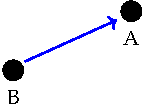
\includegraphics[]{Images/fig-RQMABcartoon.pdf}

    \caption{Consider an experiment where Bob releases a particle and Alice is some distance away. Under naive relativistic QM, Alice has a non-zero chance of measuring the particle to be at her position, even if she is so far away such that light would not be able to reach her in that time from when Bob released it.}
    \label{fig-RQMABcartoon}
\end{figure}
When we do the calculation for the probability of finding the particle some arbitrarily far distance away, we find that we have a non-zero probability regardless of the distance. To see this, let us return to the above transition probability. We can evaluate the integral approximately using the edge-of-the-wedge theorem. We note that $\bra{x_f}e^{-\frac{i}{\hbar}Ht}\ket{x_i}$ is analytic in the lower half of the complex time plane; this comes from the fact that that there the $ e^{-\frac{i}{\hbar}\sqrt{p^2c^2 + m^2c^4}t}$ leads to an exponential supression of the integral. As time comes to the real axis, it becomes much less nice (it becomes something like a distribution). We can define the value on the real axis as the limit taken from the analytic lower half time plane. How does this tell us anything? If the theory were causal, for small $t$ we would have to find that the integral is zero. But then we have some arc in the complex plane for which the function is zero. But if this region is in the region where the function is analytic, then by analytic continuation we could show that it would be zero everywhere. 

\begin{figure}[htbp]
    \centering
    \textcolor{blue}{Have: analyticity in the lower-half $t$ plane. In order for the theory to be causal, $t$ must be zero for small real $t$. But then we may use analytic continuation of the function to show that it is zero everywhere on the complex plane, since we have found an arc which it is zero on.}
    \caption{<caption>}
    \label{<label>}
\end{figure}


So the last step to show is that it is indeed analytic in this region. In the lower-$t$ plane, we can use Cauchy's integral formula to write:
\begin{equation}
    f(z_0) = \oint \frac{dz}{2\pi i}\frac{f(z)}{z - z_0}
\end{equation}
where $f = \bra{x_f}e^{-\frac{i}{\hbar}Ht}\ket{x_i}$ is our integral of interest. The value of the integral does not depend on the contour taken; let us deform the contour so that part of the contour lies on the real axis. We can then push the $z_0$ up until it is on the real axis; at this point the formula still holds, and so $f(z_0)$ is an analytic function on the real axis as well. Therefore by analytic continuation, the integral is zero everywhere. Contradiction!

\begin{figure}[htbp]
    \centering
    \textcolor{blue}{Contour integral + pushing it up}
    \caption{<caption>}
    \label{<label>}
\end{figure}

We therefore conclude that our theory violates causality. This would be ok if the universe actually behaved like this, but as far as we know we have never observed this; physics appears to be causal. So, this theory doesn't reflect reality, and we should throw it away.

\subsection{The QFT fix-up}

How does QFT fix this? First, we get the factor of $\frac{mc^2}{\sqrt{pc^2 + m^2c^4}}$ to preserve lorentz invariance. But the other thing we do is we make use of the negative energy branch of the energy spectrum:
\begin{equation}
    E = -\sqrt{p^2c^2 + m^2c^4}.
\end{equation}
When we calculate the same process in QFT, something gets added! We have two amplitudes:
\begin{equation}
    \bra{x_f}e^{-\frac{i}{\hbar}Ht}\ket{x_i} = \int \frac{d^3p}{(2\pi\hbar)^3}\left[\frac{mc^2}{\sqrt{pc^2 + m^2c^4}}e^{i\frac{\v{p}}{\hbar}\cdot(\v{x}_f - \v{x}_i) -\frac{i}{\hbar}\sqrt{p^2c^2 + m^2c^4}t} - \frac{mc^2}{\sqrt{pc^2 + m^2c^4}}e^{i\frac{\v{p}}{\hbar}\cdot(\v{x}_f - \v{x}_i) +\frac{i}{\hbar}\sqrt{p^2c^2 + m^2c^4}t}\right]
\end{equation}
i.e. we add a term that looks like time is running backwards. How do we interepret this? The first term/process has the interpretation of Bob having a particle and Alice detects it. The second term/process is as follows. When trying to detect a particle, Alice produces a particle-antiparticle pair, the antiparticle which goes the other direction and annhilates Bob's particle. We find in QFT that outside of the light cone that these two processes perfectly destructively interfere, and so causality is preserved!

An interesting note: if we repeated this analysis with a massless particle, we would find that the probability only has support on the lightcone (As we would expect; massless particles should travel on the lightcone!)

Another note: the addition of this second term destroys our analyticity argument as we now have one term that is analytic in the lower-$t$ plane and the other is analytic in the upper-$t$ plane. So we do not get the contradiction that the integral vanishes everywhere, as we did before.

Does this fixup fix everything? It seems to. They seem to be Lorentz invariant, and causal. This is why QFT gains the title of the natural marriage of quantum mechanics and special relativity (and string theory is known as the natural marriage of QM and GR - each are the only currently known solution to unifying these theories). Although this cannot be said of string theory yet, QFT at least seems to pass some very stringent experimental tests.

\subsection{Special Relativity and Minkowski Spacetime}
Once we go to a relativistic setting, it is natural to discuss space-time transformations (which are still translations, rotations and the like) which are symmetries of the space-time in which the QFT lives. We then try to write down the QFT such that these symmetries are not violated. We already know how to deal with this a little bit; we know Noether's theorem, and how to turn the crank and find conservation laws. We will therefore proceed to approach symmetries from a different point of view; as arising from the geometries of spacetime.

The space-time we consider is Minkowski spacetime; as much as we love curved spacetime, we won't consider it in this course here. It is described by coordinates:
\begin{equation}
    \v{x} = (x^1, x^2, x^3) \equiv x^a, \quad a = 1,2,3
\end{equation}
which describes three-dimensional infinite Euclidean space. The indices on the $x$s now have a position that means something. It is always up on a coordinate (or at least for the next while - $x_a$ is meaningless, for now). We will add to this another coordinate for time to make this a space-time (but we will give it units of distance to make it symmetric):
\begin{equation}
    x^0 \equiv ct
\end{equation}
where $x^0$ ranges over the real line. Combining these, we obtain a four-vector:
\begin{equation}
    x^\mu = (x^0, x^1, x^2, x^3), \quad \mu=0,1,2,3.
\end{equation}
We will generally use latin letters for regular vectors, and greek letters for four-vectors (though sometimes we leave it off entirely when the object is clear from context). The cartesian coordinates are not the only coordinates possible, but they are quite convenient; symmetries are quite apparent here.

\subsection{Coordinates on a space-time}
If we have a general spacetime, we could think about a coordinate system; all this would be is a dictionary for the various points in the spacetime, with points $x^\mu, y^\mu$ etc. There is of course a bunch of mathematical structure behind this, e.g. continuity/smoothness, this is done formally by locally mapping points (homeomorphism) to $\mathbb{R}^n$. We won't need this formality, but we will takeaway the idea of a coordinate transformation. Suppose we have a different coordinate system, with points $\tilde{x}^\mu, \tilde{y}^\mu$ etc. We could then compare dictionaries and figure out how to translate in between them. We could then define a transformation in between them: $\tilde{x}^\mu(x^\mu)$. This is a mathematical way of writing down a transformation, and the transformation inherits the ``smoothness'' of the coordinates (it is differentiable, invertible...). Formally, the invertiblity criterion is:
\begin{equation}
    \det(\frac{\partial }{\partial x^\mu}\tilde{x}^\nu) \neq 0.
\end{equation}

\subsection{Scalar Fields}
We consider a scalar field $\varphi(x^\mu)$; this is a physical entity that takes a value at each point in spacetime (for example; the temperature in a room). If someone else comes along with a different set of coordinates, we should agree with the value of the scalar field; so we should agree that:
\begin{equation}
    \varphi(x) = \tilde{\varphi}(\tilde{x})
\end{equation}
so a scalar field is defined in this way; with how it undergoes coordinate transformations.

We will discuss next time, but we can consider that displacement transforms like:
\begin{equation}
    dx^\nu = \frac{\partial x^\mu}{\partial \tilde{x}^\nu}d\tilde{x}^\nu
\end{equation}
So perhaps a vector field transforms in the same way:
\begin{equation}
    A^\mu(x) = \frac{\partial x^\mu}{\partial \tilde{x}^\nu} d\tilde{A}^\nu(x)
\end{equation}
\newpage
\section{Fields, Metrics, and Space-Time Symmetry}
\subsection{Review - Coordinates, Transformations, Scalar Fields}
Last time, we were considering a coordinate system for our spacetime (which has requirements such as smoothness that we take as a given); we have a four-vector $x^\mu$ which represents a point in the spacetime. We then considered a different coordinate system $\tilde{x}^\mu$ and a change-of-coordinates transformation $x^\mu \to \tilde{x}^\mu(x)$ (four smooth functions in four variables). This function should be invertible, with $\tilde{x}^\mu \to x^\mu(\tilde{x})$ the inverse.

We can then discuss things that live in our spacetime, such as the scalar field. The term scalar says something about this; namely it tells us how we should translate values of the field under different coordinate transformations. We have some scalar field $\varphi(x)$, and in some different set of coordinates we may have $\tilde{\varphi}(\tilde{x})$ but at the same point the data should match, so:
\begin{equation}
    \varphi(x) = \tilde{\varphi}(\tilde{x})
\end{equation}

\subsection{Vector Fields}
This is a straightforward generalization of a vector field; at each point in space we associate a vector with magnitude and direction. If temperature was an example of a scalar field, then wind would be a good example of a vector field; the wind has some magnitude and direction at each point in space. But now something to consider; when we transform between coordinates, we not only have to translate magnitudes, but also the direction of the wind. We say a (contravariant) vector field should transform like a differential:
\begin{equation}
    dx^\mu = \dpd{x^\mu}{\tilde{x}^\mu}d\tilde{x}^\nu
\end{equation}
so:
\begin{equation}
    A^\mu(x) = \dpd{x^\mu}{\tilde{x}^\nu}\tilde{A}^\nu(\tilde{x})
\end{equation}
note the up and down indices here are quite important. $x$ always has an up index. The index on the derivative is a bit interesting. We consider a transformation of the derivative:
\begin{equation}
    \dpd{}{x^\nu} = \dpd{\tilde{x}^\nu}{x^\mu}\dpd{}{\tilde{x}^\nu}
\end{equation}
and we see that this is upside-down compared to the vector field transformation; so something different is happening here. We could find a vector field that transforms under this ``upside-down'' rule, and we would distinguish this by putting a down index on it (this would be a covariant) vector field:
\begin{equation}
    A_\mu(x) = \dpd{\tilde{x}^\nu}{x^\mu}\tilde{A}_\nu(\tilde{x})
\end{equation}
Note: we remind the reader that we work with Einstein summation convention, and so when we have two indices paired they are summed over. Since the partial derivative transforms covariantly, it is natural to think of it as an object as a down index:
\begin{equation}
    \p_\mu = \dpd{}{x^\mu}, \quad \tilde{\p}_\mu = \dpd{}{\tilde{x}^\mu}
\end{equation}

\subsection{Tensor Fields}
Tensor fields are a generalization of vector fields; they are things with more than one index. One example is the inertia tensor with two indices takes the form of a 3x3 matrix in 3-dimensional space. The relativistic description of an EM field is another. We can lift our transformations of vectors into tensors in the most obvious way:
\begin{equation}
    \mathbb{T}^{\mu_1 \ldots \mu_m}\nu_{1 \ldots n}(x) = \dpd{x^{\mu_1}}{\tilde{x}^{\rho_1}}\ldots \dpd{x^{\mu_m}}{\tilde{x}^{\rho_m}} \dpd{\tilde{x}^{\sigma_1}}{x^{\nu_1}}\ldots \dpd{\tilde{x}^{\sigma_n}}{x^{\nu_n}}\tilde{\mathbb{T}}^{\rho_1 \ldots \rho_m}_{\sigma_1 \ldots \sigma_n}(\tilde{x})
\end{equation}

\subsection{Proper Time and Spacetime Metrics}
At this point, we know nothing about the spacetime beyond the fact that I know I can index it and measure things. We need more than that; we will need to embed objects into this spacetime somehow. We will need some rules for doing so, and rules thar we can all agree on.

Let's take a pet snail\footnote{Let's assume that snails exist...} and put him at $x^\mu$ in our spacetime. Now let's say he moves to $x^\mu + dx^\mu$. We then record the time that elapses on the wristwatch. This we would call the proper time. 

\begin{figure}[htbp]
    \centering
    
    \caption{<caption>}
    \label{<label>}
\end{figure}

This should vary linearly with how far he travells. We should also have a perscription for the path taken to be somehow ``sensible''; say $x^\mu + tdx^\mu$ for $0 \leq t \leq 1$. We want some way of figuring out what this proper time is. If it's linear in $x^\mu$, but this has an index and proper time is just a number. So it would be useful to square the propert time; this would be bi-linear in $x^\mu$, perhaps with an expression:
\begin{equation}
    d\tau^2 = dx^\mu g_{\mu\nu}(x)dx^\nu
\end{equation}
this defines a matrix $g_{\mu\nu}$ of some kind. It turns out to be a fairly special one; why? If we both watch the snail and record the proper time in the same way, we should agree on that proper time for every possible path he should take. We can therefore map out this matrix. Even if we restrict ourselves to timelike paths, there is enough to map out this tensor. The physics tells us that the times must agree, and so:
\begin{equation}\label{eq-dtau2WC}
    d\tau^2 = dx^\mu g_{\mu\nu}(x)dx^\nu = d\tilde{x}^\mu \tilde{g}_{\mu\nu}(\tilde{x})d\tilde{x}^\nu
\end{equation}
This tells us that $g$ transforms as a tensor field! And so:
\begin{equation}
    g_{\mu\nu}(x) = \dpd{\tilde{x}^\rho}{x^\mu}\dpd{\tilde{x}^\sigma}{x^\nu}\tilde{g}_{\rho\sigma}(\tilde{x}).
\end{equation}
We give this tensor field a name of being a \emph{metric}, or \emph{metric tensor}. This encodes a lot of information about our spacetime, as it in a sense measures distances. We will not go into the direction of curvature and general relativity here, but this is certainly a fascinating direction. 

\subsection{Minkowski Spacetime}
We are only example in a specific example of spacetime - Minkowski spacetime. We define it as a spacetime where there exists a coordinate system such that:
\begin{equation}
    g_{\mu\nu}(x) = \m{-1& 0 & 0 & 0 \\ 0 & 1 & 0 & 0 \\ 0 & 0 & 1 & 0 \\ 0 & 0 & 0 & 1}
\end{equation}
the poor snail notices that there are limits on his motion coming from the minus sign; he cannot for example go backwards in time. Note we have to correct the formula in Eq. \eqref{eq-dtau2WC} we had for $d\tau^2$ due to this minus sign:
\begin{equation}
    d\tau^2 = -dx^\mu g_{\mu\nu}(x)dx^\nu = -d\tilde{x}^\mu \tilde{g}_{\mu\nu}(\tilde{x})d\tilde{x}^\nu
\end{equation}
Note that this is known as the east-coast convention; one could alternatively take:
\begin{equation}
    g_{\mu\nu}(x) = \m{1& 0 & 0 & 0 \\ 0 & -1 & 0 & 0 \\ 0 & 0 & -1 & 0 \\ 0 & 0 & 0 & -1}
\end{equation}
and this would be the west-coast convention. Despite our location at UBC, we adopt the east-coast convention.

Some background; the WC convention was developed by high-energy physicists, while the EC convention was developed by relativists. The former has the benefit of energies being positive, the latter has the benefit of distances being positive. Both are correct and often one takes the convention most convenient for the setting (depending on whether you discuss particle energies, or geometry).

\subsection{Infinitesimal Coordinate Transformations}
We consider infinitesimal coordinate transformations:
\begin{equation}
    \tilde{x}^\mu = x^\mu + f^\mu(x)
\end{equation}
We can think of $f^\mu$ as small but otherwise arbitrary. It also looks like a vector field, but is not quite one (it coordinate transforms in a funny way). Scalar fields transform under infinitesimal transformations as:
\begin{equation}
    \varphi(x) = \tilde{\varphi}(\tilde{x}) = \varphi(x) + \delta \varphi(x) + f^\mu(x)\p_\mu\varphi(x)
\end{equation}
where we have Taylor expanded in $f$ for the last term. As usual we consider only up to linear order. Cancelling terms, we obtain:
\begin{equation}
    \delta \phi(x) = -f^\mu(x)\p_\mu\phi(x)
\end{equation}
We can then abstract this to various other fields. One example is the contravariant vector field:
\begin{equation}
    A^\mu(x) = \dpd{x^\mu}{\tilde{x}^\nu}\tilde{A}^{\nu}(\tilde{x})
\end{equation}
Note the beauty of infinitesimal transformations in that they are very easy to invert:
\begin{equation}
    x^\mu = \tilde{x}^\mu - f^\mu(\tilde{x})
\end{equation}
and so
\begin{equation}
    \dpd{x^\mu}{\tilde{x}^\nu} = \delta^\mu_\nu - \p_\nu f^\mu
\end{equation}
therefore:
\begin{equation}
    A^\mu(x) = A^\mu(x) - \p_\nu f^{\mu}(x)A^\nu(x) + \delta A^\mu(x) + f^\nu(x)\p_\nu A^\mu(x)
\end{equation}
From here the zeroth order bit cancells out, and so:
\begin{equation}
    \delta A^\mu(x) = -f^\nu\p_\nu A^\mu(x) + \p_\nu f^\mu(x)A^\nu(x)
\end{equation}
where the first term comes from the transformation of the coordinate and the second term comes from the transformation of the frame. The scalar field has the first part (and in fact every field will have it)! The extra terms are the derivatives of the transformation function with the indices matched up. Doing the same for covariant fields:
\begin{equation}
    \delta A_\mu(x) = -f^\nu(x)\p_\nu A_\mu(x) - \p_\mu f^\nu(x) A_\nu(x)
\end{equation}
And as a particular example, the metric transforms as:
\begin{equation}
    \delta g_{\mu\nu}(x)=  - f^\lambda(x)\p_\lambda g_{\mu\nu}(x) - \p_\mu f^\lambda(x) g_{\lambda \nu}(x) - \p_\nu f^\lambda(x) g_{\mu\lambda}(x)
\end{equation}

\subsection{The definition of space-time symmetry}
Having discussed metrics, what else can one say about a space? One thing that would be interesting is symmetry. Maybe we can define symmetry of spacetime as follows; symmetry is a change of coordinates such that the rules for calculating proper time remain exactly the same. We need the metric to calculate the proper time; so if we calculate the same proper time under a coordinate transformation, the metric better be left identical. Putting this together, we can say that \emph{A symmetry of space-time is a coordinate transformation such that $\delta g_{\mu\nu}(x) = 0$}. So to discover symmetries, we can dream up a large class of $f$s, and see for what class we have $\delta g_{\mu\nu}(x) = 0$. This wouldn't be a useful definition of symmetry was plentiful, and in general it is quite rare to find them. Precisely, the maximum number of spacetime symmetries turns out to be $d(d+1)/2$\footnote{The number of independent components of a $d\times d$ symmetric tensor - though typically there are less, there are only 3 maximally symmetric spaces, namely Minkowski, and the spaces of constant positive or constant negative curvature. For 2D surfaces, this means the only maximally symmetric surfaces are the plane, sphere, and the one that looks locally like a Pringle (I missed the formal name that Gordon said here). In 4D we have Minkowski, DeSitter and Anti DeSitter space.}. This is obtained by counting the solutions to the differential equation obtained by setting $\delta g_{\mu\nu}(x) = 0$. An equivalent definition of symmetry is therefore: \emph{$\hat{f}^\mu(x)$ is a symmetry if:
\begin{equation}
    \hat{f}^\lambda(x)\p_\lambda g_{\mu\nu}(x) + \p_\mu \hat{f}^\lambda(x) g_{\lambda \nu}(x) + \p_\nu \hat{f}^\lambda(x) g_{\mu\lambda}(x)
\end{equation}
i.e. $\hat{f}^\mu(x)$ the Killing vector satisfies the Killing equation.} One might wonder if the form of the equation changes in different coordinate systems; this turns out to not be the case (and would require some differential geometry knowledge). This gives us a systematic way to discuss symmetries; something we will continue with next class.
\newpage
\section{Symmetries of Minkowski Space-Time, Conformal Transformations}
\subsection{Metric Tensors}
We have been discussing the metric tensor field $g_{\mu\nu}(x)$. This is special because it is used to measure proper times. There is one small thing we have forgot to mention which we should now fill in. What is $g^{\mu\nu}(x)$? The way we define this is the inverse of the metric with down indices. Therefore:
\begin{equation}
    g^{\mu\nu}(x)g_{\mu\lambda}(x) = \delta^\mu_\lambda
\end{equation}w
here $\delta^\mu_\lambda$ is the $4 \times 4$ matrix with ones on the diagonal and zeros everywhere else. We can study how this transforms (and the answer is: it will not!)
\begin{equation}
    \delta^\mu_\lambda = \dpd{x^\mu}{\tilde{x}^\rho}\dpd{\tilde{x}^\sigma}{x^\lambda}\tilde{\delta}^\sigma_\rho
\end{equation}
the above equation only holds if $\tilde{\delta}^\sigma_\rho$ is identically a unit matrix. So, it looks the same in every coordinate system. It is sometimes called an \emph{invariant tensor} for this reason (of which there are fairly few). 

Note that $g^{\mu\nu}$ is also a tensor (a contravariant one).

Note that we have here assumed that the metric is invertible. If it is not, then our proper time experiments would have some strange results indeed... the snail could travel and no time could pass on the wristwatch, for example. This doesn't seem very physical. So we say that this shouldn't be possible; the metric should be invertible everywhere (technical terminology: the metric should be non-degenerate).

\subsection{Contracting Fields, Raising/Lowering Indices}
We can consider the contraction of two vector fields:
\begin{equation}
    A_\mu(x)A'^{\mu}(x)
\end{equation}
this object transforms like a scalar field; this makes sense, as it should transform like something without any indices.

In the same vein, once we have this tensor $g$, we can use it to raise indices on vector (tensor) fields:
\begin{equation}
    A^\mu(x) = g^{\mu\nu}(x)A_\nu(x)
\end{equation}
and similarly:
\begin{equation}
    A_\mu(x) = g_{\mu\nu}A^{\nu}(x)
\end{equation}

A note: haven't discussed spinors and their transformations; this is because there isn't really a transformation law for them. This might be a bit disquieting that this simple structure we have been exploring does not cover all possible physical objects (e.g. electrons are described by spinors). This will eventually be something we need to consider.

\subsection{Symmetries of Space-Time}
A symmetry of space-time is a coordinate transformation:
\begin{equation}
    x^\mu \to \tilde{x}^\mu = x^\mu + f^\mu(x)
\end{equation}
that leaves the metric invariant:
\begin{equation}
    \delta g_{\mu\nu}(x) = 0.
\end{equation}
So literally, $g$ looks the same in both coordinate systems. We can't tell if we are doing physics in one coordinate systems or the other. 

An example of a coordinate transformation that \emph{isn't} a symmetry: the transformation that takes us from cartesian to polar coordinates. This is \emph{not} a symmetry transformation. The schrodinger equation looks different in this coordinate system!

An example of a coordinate transformation that \emph{is} a symmetry: a transformation that rotates/changes the direction of the Cartesian axes. In this case the laws of physics look exactly the same.

We can write explicitly the Killing equation:
\begin{equation}
    \hat{f}^\lambda(x) \p_\lambda g_{\mu\nu}(x) + \p_\mu \hat{f}^\lambda(x) g_{\lambda\nu}(x) + \p_\nu \hat{f}^\lambda(x) g_{\mu\lambda}(x) = 0.
\end{equation}
The solutions $\hat{f}^\lambda(x)$ of which are called Killing vectors.

\subsection{Killing Equation and Vectors for Minkowski Space-Time}
Let's look at the Killing vectors for Minkowski space. Recall that Minkowski space is defined by the fact that we can go to a coordinate system where the metric looks like:

\begin{equation}
    g_{\mu\nu}(x) = \eta_{\mu\nu} = \m{-1 & 0 & 0 & 0 \\ 0 & 1 & 0 & 0 \\ 0 & 0 & 1 & 0 \\ 0 & 0 & 0 & 1}
\end{equation}

We can plug this into the equation and find the Killing equation for Minkowski space:
\begin{equation}
    \p_\mu f^\lambda \eta_{\lambda\mu} + \p_\nu f^\lambda \eta_{\mu\lambda} = 0.
\end{equation}
If we now define:
\begin{equation}
    \hat{f}_\mu(x) = \eta_{\mu\nu}\hat{f}^\nu(x)
\end{equation}
then the Killing equation reads:
\begin{equation}
    \p_\mu \hat{f}_\nu + \eta_\nu \hat{f}_\mu = 0.
\end{equation}
and we can start searching for our Killing vectors. Note that the above is a homogenous equation, which helps us with our search (we can look for solutions of zeroth order and linear order). They are:
\begin{enumerate}
    \item $\hat{f}_\mu = C_\mu$, constants (of which there are 4). These correspond to time and space translation symmetry.
    \item $\hat{f}_\mu  = \omega_{\mu\nu}x^\nu$. We observe that this is indeed a solution with $\omega_{\mu\nu}$ anti-symmetric, so $\omega_{\mu\nu} = -\omega_{\nu\mu}$. These are the Lorentz transformations (in the broader sense); 3 spatial rotations and 3 Lorentz boosts.
\end{enumerate}
Higher order polynomials do not solve the equation; this is it! This is as many Killing vectors as a space-time can have (Minkowski space is maximally symmetric) - there are 10 total for $D = 4$.

\subsection{Conformal Transformations}
Under a conformal transformation, the rules change slightly (this is a slight extension of our concept of symmetry). This is important as there are some QFTs that have this kind of enhanced symmetry (not technically a symmetry of the space as we have defined it). Conformal transformations are coordinate transformations for which the metric transforms to something proportional to the metric:
\begin{equation}
    \delta g_{\mu\nu}(x) = \Omega(x) g_{\mu\nu}(x).
\end{equation}
This is the Conformal Killing equation. In Minkowski space, it looks like:
\begin{equation}
    \p_\mu \hat{f}_\nu(x) + \p_\nu \hat{f}_\mu (x) - \frac{2}{D}\eta_{\mu\nu}\p_\lambda \hat{f}^\lambda (x) = 0.
\end{equation}
Where $D$ is the dimension of the space. One can check that the Killing vectors for Minkowski space are divergence free, so the third term vanishes and (of course) we have that the original Killing equation is satisfied. How many additional solutions are there? Not too many. Again it is homogenous so we can try the same strategy of looking for polynomial solutions. We find the conformal Killing vectors:
\begin{enumerate}
    \item $\hat{f}_\mu  C_\mu$
    \item $\hat{f}_\mu = \omega_{\mu\nu}x^\nu$ for $\omega$ antisymmetric.
    \item $\hat{f}^\mu = \lambda x^\mu$. A scale transformation.
    \item $\hat{f}^\mu = x^\mu x^\nu b_\nu - b^\mu \frac{x^\nu x_\nu}{2}$ where $b$ is some constant four-vector (of which there are four possible choices).
\end{enumerate}
In the above, we have $x$ with a lower index. It is defined as:
\begin{equation}
    x_\nu = \eta_{\mu\nu}x^\mu
\end{equation}
once we are in Minkowski space and agree on using Cartesian coordinates, we can raise and lower the indices on $x$ (and on anything) with $\eta$. We can think of this as an inner product/space-time invariant:
\begin{equation}
    x^\nu x_\nu = \eta_{\mu\nu}x^\mu x^\nu = \v{x}^2 - (x^{0})^2
\end{equation}
and this may be familiar from a previous course in special relativity.

As discussed before, conformal invariance can give us some extra symmetries when studying some systems; e.g. the classical Ising model on its second order phase transition; this turns out to be a QFT with $\hbar = 1$! It's not a quantum system, yet it obeys the rules of a QFT with a conformal symmetry. The conformal symmetry and some of its constraints have been exploited to calculate the critical exponents of the Ising model to world-record accuracy, matching numerical simulations perfectly.

\subsection{Finite Lorentz Transformations}
So, we've discussed the infinitesimal transformations. Let's say a few words about the finite case. We consider the Lorentz transforms:
\begin{equation}
    x^\mu \to \tilde{x}^\mu = x^\mu + \omega^\mu_\nu x^\nu
\end{equation}
So we write this as:
\begin{equation}
    \tilde{x}^\rho = \Lambda^\rho_{\mu}x^\mu
\end{equation}
where:
\begin{equation}
    \Lambda_\mu^\rho \approx \delta^\rho_\mu + \omega^\rho_\mu
\end{equation}
We consider the corresponding transformation for the metric:
\begin{equation}
    \eta_{\mu\nu} = \dpd{\tilde{x}^\rho}{x^\mu}\dpd{\tilde{x}^\sigma}{x^\mu}\eta_{\rho\sigma} = \Lambda^\rho_\mu \Lambda^\sigma_\nu \eta_{\rho\sigma}
\end{equation}
Lorentz transformations are the set of all $\Lambda$s which obey the above equation. We have been studying the infinitesimal ones. We know that:
\begin{equation}
    (\det \Lambda)^2 = 1
\end{equation}
and so:
\begin{equation}
    \det \Lambda = \pm 1
\end{equation}
The $\det \Lambda = 1$ transformations are known as proper. It can be shown that the $\Lambda$s here form a group. If $\Lambda_1, \Lambda_2$ obey the equation, then so do $\Lambda_1^{-1}$, $\Lambda_1\Lambda_2$ etc.

(Some comment about objects that are invariant under Lorentz transformations, e.g. $A^\mu(x)A_\mu(x)$, that I didn't really understand).
\newpage
\section{Real Scalar Field Theory}
We've been discussing special relativity; now we use it to build up our relativistic quantum field theory. When we discussed our non-relativistic QFT, we didn't discuss geometry all too much; but here it will be useful to inform us about the kinds of space-time symmetries that our theory should possess as well. Our world doesn't look fairly symmetric; that said physics has had quite a bit of success exploring theories with symmetries to explain our universe; and elementary particle physics does appear to possess these.

\subsection{Setting up the Real Scalar Field Theory}

Let's look at a simple (in fact the simplest) example of a relativistic QFT. This will be simple in the sense that we will not have to worry about many indices. We consider a real scalar field theory. Consider a scalar field $\varphi(x)$, and we want to consider a dynamical system where $\varphi$ is a degree of freedom, and is relativistic. We can start writing down the Lagrangian density guided by what we have learned in the last few lectures. Some are convention dependent; there could be derivative terms in $\varphi$, and these are usually written first. The normalization of the derivative term fixes the normalization of the field $\varphi$, as well. We want to organize the derivatives such that they have Lorentz symmetry. We thus obtain the term:

\begin{equation}
    -\frac{1}{2}\p_\mu \varphi(x)\p^\mu \varphi(x)
\end{equation}

We could have terms with more derivatives (so-called effective field theories); while they would not be excluded in classical field theories, quantum field theories do not like them very much; so we do not consider them. We also could have something quadratic in $\varphi$:
\begin{equation}
    -\frac{m^2}{2}\varphi^2(x)
\end{equation}

We could in principle have a term linear in $\varphi$, but we can get rid of it assuming that the Lagrangian has a symmetry such that it is unchanged under replacing $\varphi$ with $-\varphi$.

There are other terms that could contain $\varphi$, such as:
\begin{equation}
    -\frac{\lambda}{4!}\varphi^4(x)
\end{equation}

(of course all the odd terms have to vanish by the $-\varphi \leftrightarrow \varphi$ symmetry). Of course we could have in principle $\varphi^6, \varphi^8$ terms etc. but these are not allowed due to renormalizability conditions. So in principle we have written everything down that could be contained in our Lagrangian density:
\begin{equation}
    \L = -\frac{1}{2}\p_\mu \varphi(x) \p^\mu \varphi(x) - \frac{m^2}{2}\varphi^2(x) - \frac{\lambda}{4!}\varphi^4(x)
\end{equation}
We have tried to organize the Lagrangian density such that it transforms like a scalar under Lorentz transformations. Let's begin by studying what this Lagrangian tells us. The Euler-Lagrange equation in relativistic form for a scalar field is very nice; it reads:
\begin{equation}
    \p_\mu \dpd{\L}{(\p_\mu \varphi(x))} = \dpd{\L}{\varphi(x)}
\end{equation}
We thus find the equation of motion:
\begin{equation}\label{eq-realscalarfieldEOM}
    (-\p^2 + m^2)\varphi(x) + \frac{\lambda}{3!}\varphi^3(x) = 0.
\end{equation}
For $\lambda$ finite this is very hard to solve, so in general the approach is to treat this in perturbation theory with small $\lambda$. If we set $\lambda = 0$, we obtain the Klein-Gordon equation:
\begin{equation}
    (-\p^2 + m^2)\varphi(x) = 0.
\end{equation}
and this term in \eqref{eq-realscalarfieldEOM} is the Klein-Gordon term, with wave operator $-\p^2 + m^2$. The $\frac{\lambda}{3!}\varphi^3(x)$ non-linear term can be thought of the interaction term. This is in analogy to our previous non-relativistic QFT, where we had a free field equation and added on the interaction terms. Note there isn't really a place here for an operator ordering ambiguity; everything commutes with everything here. 

\subsection{Natural Units}
We work in a system of units where $\hbar = 1, c = 1$. Note that if we had not made this choice, then there would be factors of $\hbar, c$ in the $- \frac{m^2}{2}\varphi^2(x)$ term. We can of course figure out where these should go by studying the units, but with natural units we are saved the hassle.

\subsection{Commutation Relations}
Note that this is the kind of system where the Lagrangian has velocity squared times some function of position:
\begin{equation}
    \L = \frac{1}{2}\dpd{\varphi}{t}\dpd{\varphi}{t} + \ldots 
\end{equation}
so the canonical momentum is $P = \dpd{\varphi}{t}$, and the canonical position $X = \varphi$. We then have the Poisson bracket:
\begin{equation}
    \{\varphi, \dpd{}{t}\varphi\} = \delta()
\end{equation}
and lifting this to the QFT, we have the commutator relation:
\begin{equation}
    [\varphi(x), \dpd{}{t}\varphi] = i\hbar \delta()
\end{equation}
Concretely, we have the equal-time commutation relations of:
\begin{equation}
    [\varphi(x), \dpd{}{y^0}\varphi(y)]\delta(x^0 - y^0) = i\delta(x - y)
\end{equation}
Of course the positions commute with each other:
\begin{equation}
    [\varphi(x), \varphi(y)]\delta(x^0 - y^0) = 0
\end{equation}
As do the momenta:
\begin{equation}
    [\dpd{}{x^0}\varphi(x), \dpd{}{y^0}\varphi(y)]\delta(x^0 - y^0) = 0
\end{equation}
One might wonder if particle physicists are missing any theories by only considering Lagrangian ones; but this is a discussion for another day.

\subsection{Symmetry}
We recall the infinitesimal transformation of the scalar field:
\begin{equation}
    \delta \varphi(x) = -f^\mu(x)\p_\mu \varphi(x)
\end{equation}
where if this is a space-time symmetry then $f^\mu$ is a Killing vector; otherwise it is a generic change of coordinates. Let us keep it general for now; we see from algebra that:
\begin{equation}
    \delta \L(x) = -f^\mu(x)\p_\mu \L(x) + (\p_\mu f_\nu + \p_\nu f_\mu)\frac{1}{2}\p^\mu \varphi \p^\nu \varphi
\end{equation}
We need to show that this transforms like the derivative of something. So let us rearrange using the product rule:
\begin{equation} 
    \delta \L(x) = \p_\mu (-f^\mu(x)\L(x)) + (\p_\mu f_\nu + \p_\nu f_\mu)\frac{1}{2}\left(\p^\mu \varphi \p^\nu \varphi + \eta^{\mu\nu}\L\right)
\end{equation}
Now if $f^\mu$ is a Killing vector, then $\p_\mu f_\nu + \p_\nu f_\mu = 0$ from the Killing equation in Minkowski space! So $\delta \L$ can be written as a total derivative - it is a symmetry in the Noetherian sense if $f^\mu$ is a Killing vector/we have a space-time symmetry:
\begin{equation}
    \delta \L(x) = -f^\mu(x) \p_\mu \L(x)
\end{equation}
Applying Noether's theorem, we can obtain the Noether charge density and current. By Noether's theorem:
\begin{equation}
    \gv{\mathcal{J}}^\mu = \delta\varphi \dpd{\L}{\p_\mu\varphi} - \mathcal{R}^\mu = \hat{f}^\nu \p_\nu \varphi \p^\nu \varphi + \hat{f}^\mu\L
\end{equation}
where $\mathcal{R}^\mu = (R, \v{J})$ from our old formulation of Noether's theorem (not in relativistic notation). So by Noether's theorem, this is conserved:
\begin{equation}
    \p_\mu \gv{\mathcal{J}}^\mu = 0.
\end{equation}

\subsection{A Faster Noether's Theorem}
We came here with a variation of $\phi$ where $f$ was arbitrary, obtaining:
\begin{equation}
    \delta \L(x) = \p_\mu (-f^\mu(x)\L(x)) + (\p_\mu f_\nu + \p_\nu f_\mu)\frac{1}{2}\left(\p^\mu \varphi \p^\nu \varphi + \eta^{\mu\nu}\L\right)
\end{equation}
Now, what if we actually imposed the equation of motion (something we have been told not to do)? If we vary the Lagrangian density and impose the the equations of motion (from the EL equation), then the above variation in $\L(x)$ has to be written as a total derivative. How do we make th esecond term in the above expression a total derivative? By writing $\p_\mu(\ldots)$ and $\p_\nu()$... but then this implies the $\p_\mu\left(\p^\mu \varphi \p^\nu \varphi + \eta^{\mu\nu}\L\right) = 0$ which gives us the result in a quick way! 

\subsection{The Stress Tensor}
Another connection; let us write the Noether current as a contraction of the Killing vector:
\begin{equation}
    \gv{\mathcal{J}}^\mu = \hat{f}^\nu \left(\p_\nu \phi \p^\mu \phi  + \eta_{\nu}^\mu \L\right)
\end{equation}
We may call the above expression in the brackets a stress tensor $\mathbb{T}_{\nu}^\mu(X)$ and from the conservation:
\begin{equation}
    \p_\mu \mathbb{T}^{\mu\nu}(x) = 0.
\end{equation} 

So, in our context here we have the Stress tensor definition:
\begin{equation}
    \mathbb{T}^{\mu\nu}(x) = \p_\nu \phi \p^\mu \phi  + \eta_{\nu}^\mu \L
\end{equation}

So: the Nother current for a symmetry $\delta \phi = -\hat{f}^\mu \p_\mu \phi$  is:
\begin{equation}
    \gv{\mathcal{J}}^\mu = \hat{f}_\nu (x) \mathbb{T}^{\mu\nu}(x).
\end{equation}
and this conserved stress tensor summarizes the conservation laws of spacetime symmetries. There are no operator ordering ambiguities, and the theory is not constructed to have any other symmetries, so we are in some sense done. But we still learn things. The time-time component gives the energy density, the time-space component gives the momentum density, and the other components give us stresses/strains and so on. Recall we also had this in non-relativistic physics, and this is exactly the analog. The construction of things like angular momentum operators from $\mathbb{T}$ in the non-relativistic setting generalizes here, by considering the various space-time symmetries of the form:
\begin{equation}
    \hat{f}_\nu(x) = C_\nu + \omega_{\nu\lambda}x^\lambda.
\end{equation}

\subsection{Non-Interacting Theory}
In order to gain intuition, let us try to solve this theory in the limit where it is solvable, i.e. when we set the nonlinear term to $\lambda = 0$. In this case, the field equation looks as follows:
\begin{equation}
    (-\p^2 + m^2)\phi(x) = 0
\end{equation}
This can be solved (as usual) by the plane wave ansatz:
\begin{equation}
    \phi(x) \sim e^{ik_\mu x^\mu}
\end{equation}
this solves the equation if:
\begin{equation}
    k^\mu k_\mu + m^2 = 0.
\end{equation}
Which tells us the relativistic dispersion relation:
\begin{equation}
    k^0 = \pm \sqrt{\v{k}^2 + m^2}
\end{equation}
We need both solutions. The plane waves are intrinsically complex, but of course $\phi$ is an intrinsically real scalar field, i.e. $\phi = \phi^*$ in classical field theory of $\phi = \phi^\dag$ in quantum field theory. We need plane waves on both sides to superimpose them and cancel out the imaginary components:
\begin{equation}
    \phi(x) = \int \frac{d^3k}{\sqrt{(2\pi)^3 2\omega(k)}}\left(e^{i\v{k}\cdot \v{x} - i\omega t}a(\v{k}) - e^{-i\v{k}\cdot\v{x} + i\omega t}a^\dag(\v{k})\right)
\end{equation}
where $\omega(k) = \sqrt{k^2 + m^2}$. One could check that the plane waves were complete, orthonormal (and so on) and that this is a solution to the QFT. In the QFT the $a, a^\dag$s become operators with commutation relations:
\begin{equation}
    [a(\v{k}), a^\dag(\v{l})] = \delta^3(\v{k} - \v{l})
\end{equation}
which implies that:
\begin{equation}
    [\phi(x), \dpd{}{y^0}\phi(y)]\delta(x^0 -y^0) = \delta^3(\v{x} - \v{y})
\end{equation}

In fact if we look at the Hamiltonian:
\begin{equation}
    H = \int d^3x \mathbb{T}^{00}(x)
\end{equation}
and we plug in our solution and do some algebra, we find:
\begin{equation}
    H = \int d^3k \omega(\v{k})a^\dag(\v{k})a(\v{k}) + C
\end{equation}
i.e. a bunch of (non-interacting) harmonic oscillators plus a constant (which comes from the operator ordering), which many QFT courses tell you is harmless (as we are only interested in relative energies) but is not quite physically true... of course we have things like gravity which depend on the total energy density. But since we don't feel ourselves gravitating to some infinite energy density from the scalar field, then we should set it to zero to be consistent with physics:
\begin{equation}
    H = \int d^3k \omega(\v{k})a^\dag(\v{k})a(\v{k}).
\end{equation}

This in some sense is an ambiguity of the theory (and one of the mysteries of QFT)! It is an arbitrary constant, but gets a bit hairy when you think about it too much; e.g. the dark energy density in our theory here would be infinite, but it is finite in our universe. We won't need it for anything because we won't be venturing off into quantum gravity, but it would be important there.

The momentum are:
\begin{equation}
    P^a = \int d^3x \mathbb{T}^{0a}(x) = \int d^3k k^a a^\dag(\v{k})a(\v{k}) + C
\end{equation}
here we might be able to argue that the constant is zero by an isotropy argument, but we run into troubles with frame dependence etc.... but let us not worry about it too much and just set it to zero.

Finally, let us construct quantum states for our theory. We have the vacuum $\ket{0}$, which is normalized:
\begin{equation}
    \braket{0}{0} = 1
\end{equation}
and is annhilated by the annhilation operators:
\begin{equation}
    a(\v{k})\ket{0} = 0, \quad \bra{0}a^\dag(\v{k}) = 0 \quad \forall \v{k}
\end{equation}
We then have our basis:
\begin{equation}
    \set{\ket{0}, a^\dag(\v{k})\ket{0}, \frac{a^\dag(\v{k}_1)a^\dag(\v{k}_2)\ket{0}}{\sqrt{2}}, \ldots }
\end{equation}
and we now more or less have a complete solution of our theory. As soon as we turn on $\lambda$ we have no solution, but can obtain a solution via perturbation theory, where we learn how to include corrections. The whole course here on in is learning how to include these corrections in a systematic way, and in fact this is all we know how to do (other than trying to solve the theory numerically). For this particular theory, things have been studied up to $\lambda^8$, with roughly $8!$ Feynman diagrams...
\newpage
\section{Correlation Functions, Real Scalar Field Theory II}
\subsection{A Review of Defining Field Theories}
The discussion is getting excited! We are finally getting to a non-relativistic quantum field theory; albeit one that we are not, in general, able to solve. However, it is a fact that there are very few solvable field theories. They tend to have special properties, e.g. be in dimension 1 (can still be useful for studying some QM systems) but the systems for which QFT was developed for (i.e. Quantum Electrodynamics) is analytically unsolvable. So our procedure will be to remove the interactions, solve it exactly, and add back the interactions in perturbation theory. And this is basically the state of the art; doing free field theory and perturbation theory on top. And standard model/particle physics is basically based completely on this.

We also had a few different presentations of our theory. We began by writing down a Lagrangian that looks symmetric. Then if there is any doubt, we check that this is indeed the case. This then defines the field theory, as all of the data of the field theory is encoded in the Lagrangian (really the Lagrangian density, but the entire world calls it the Lagrangian). For our free real scalar field theory, we had:
\begin{equation}\label{eq-freescalarfieldtheorylagrangian}
    \L = -\frac{1}{2}\p_\mu \varphi \p^\mu \varphi - \frac{m^2}{2}\varphi^2
\end{equation}
We alternatively could take our starting point as the field equation and commutation relations:
\begin{equation}\label{eq-kgeqn}
    (-\p^2 + m^2)\varphi = 0
\end{equation}
\begin{equation}\label{eq-freescalarfieldtheorycommutations}
    [\varphi(x), \dot{\varphi}(y)]\delta(x^0 - y^0) = i\delta^3(\v{x} - \v{y})
\end{equation}
but the Lagrangian method gives us a little more structure from Noether's theorem. We could be clever and guess the conservation laws using the field equation/commutation relation approach, but we would have to be quite clever. Today, we will want to discuss yet a third way of encoding the data of the field theory; and that is in correlation functions.

\subsection{Correlation Function Definition of Field Theories}
By a correlation function, we mean:
\begin{equation}
    \bra{0}\varphi(x_1) \ldots \varphi(x_n)\ket{0}
\end{equation}
and another way to write down our QFT is to write down all possible correlation functions. At first this seems like a clumsy way to proceed; in the other methods we can write down the theory in a few lines. In this method we have an (infinite) set of correlation functions to write down. Fortunately, there will be a great simplifying principle.

This set of expectation values are given the name of Wightmom functions (Wightmom being a scientist who tried to axiomatize field theories - to some small level of success). We therefore write:
\begin{equation}
    W(x_1 \ldots x_n) = \bra{0}\varphi(x_1) \ldots \varphi(x_n)\ket{0}
\end{equation}
Note that we will like to consider time-ordered correlation functions:
\begin{equation}
    \bra{0}T\varphi(x_1) \ldots \varphi(x_n)\ket{0}
\end{equation}
where $T$ is an operator that orders the $\varphi(x_i)$s to go from earlier to later times. This is nice as it makes the correlator symmetric in the $x$s. This was realized by Dyson early on in modern field theory, who noticed that time-dependent perturbation theory in QFT simplifies significantly if correlation functions are written in this time-ordered form. For this reason they are called Dyson correlation functions, and we denote:
\begin{equation}
    \Gamma(x_1 \ldots x_n) = \bra{0}T\varphi(x_1) \ldots \varphi(x_n)\ket{0}
\end{equation}
and these $\Gamma$s tend to be the useful/tractable correlation functions that we will generally consider.

There are places where this formulation of field theory is useful, e.g. in Monte Carlo approaches to field theories.

\subsection{Returning to our Real Scalar Relativistic Free  Field Theory}
Last time we found that our real scalar relativistic free field theory (with Lagrangian in Eq. \eqref{eq-freescalarfieldtheorylagrangian} and field equation/commutation relations given in Eqs. \eqref{eq-kgeqn}, \eqref{eq-freescalarfieldtheorycommutations}) and we found the solutions to be:
\begin{equation}
    \varphi(x) = \int \frac{d^3k}{\sqrt{(2\pi)^3 2\omega(\v{k})}}\left(e^{i\v{k}\cdot \v{x} - i\omega t}a(\v{k}) - e^{-i\v{k}\cdot\v{x} + i\omega t}a^\dag(\v{k})\right)
\end{equation}
with commutation relations:
\begin{equation}
    [a(\v{k}), a^\dag(\v{l})] = \delta^3(\v{k} - \v{l})
\end{equation}

Note that there are other conventions for the $\frac{1}{\sqrt{2\omega(\v{k})}}$; we have a real scalar field, so it should be invariant under Lorentz transformations. But the $\delta(\v{k} - \v{l})$ and the $a$s do not. So we introduce the $\frac{1}{\sqrt{2\omega(\v{k})}}$ in our free field theory solution to compensate for the weird transformations that the $a$s obey. At this point, some textbooks avoid this problem by introducing a different normalization for the commutators:
\begin{equation}
    [a(\v{k}), a^\dag(\v{l})] = 2\omega(\v{k})\delta^3(\v{k} - \v{l})
\end{equation}
and then the integration measure:
\begin{equation}
    \int \frac{d^3k}{2\omega(\v{k})}
\end{equation}
would be Lorentz invariant. So there is a more invariant way to write all of these things. It is left as an exercise to the reader tha the above is a Lorentz invariant measure, and that $2\omega(\v{k})\delta^3(\v{k} - \v{l})$ is Lorentz invariant.

Here we have an explicit solution to the theory! We have a vacuum state $\ket{0}$ where:
\begin{equation}
    a(\v{k})\ket{0} = 0 \quad \forall \v{k}
\end{equation}
we also have the dual statement:
\begin{equation}
    \bra{0}a^\dag(\v{k}) = 0 \quad \forall \v{k}
\end{equation}
And then we can establish a basis:
\begin{equation}
    \set{\ket{0}, a^\dag(\v{k})\ket{0}, \frac{a^\dag(\v{k}_1)a^\dag(\v{k}_2)\ket{0}}{\sqrt{2}}, \ldots }
\end{equation}
And there is of course a natural inner product we get in this space we get from contracting with the dual and using the commutation relations and so on. We then would investigate Cauchy sequences and all of their limits, and then the space of all Cauchy sequences + their limits gives us the Hilbert space we want. These details aren't needed really, but they are of course there. As we discussed previously, we can write down the energy-momentum tensor and from there obtain things such as the momentum and the Hamiltonian:
\begin{equation}
    P^\mu = \int d^3 x T^{0\mu}(x) 
\end{equation}
and so:
\begin{equation}
    P^0 = H = \int d^3k \omega(\v{k})a^\dag(\v{k})a(\v{k})
\end{equation}
\begin{equation}
    \v{P} = \int d^3k \v{k}a^\dag(\v{k})a(\v{k})
\end{equation}

\subsection{Transformations of the Real Scalar Field}
note that we can therefore find:
\begin{equation}
    [P^\mu, \varphi(x)] = i\p^\mu \varphi(x)
\end{equation}
i.e. the momentum generates some space-time translation of the field! We could also write down a Noether charge corresponding to Lorentz invariance
\begin{equation}
    M^{\mu\nu} = \int d^3x(x^\mu T^{0\nu} - x^\nu T^{0\mu})
\end{equation}
which looks a lot like the angular momentum operator we are familiar with. We could then calculate:
\begin{equation}
    [M^{\mu\nu}, \varphi(x)] = i(x^\mu p^\nu - x^\nu \p^\mu)\varphi(x)
\end{equation}
(note that in the above computation we can set the time to be whatever we like; $t=0$ may be convenient). So we have the infinitesimal Lorentz transformations. In more detail:
\begin{equation}
    \Lambda^\mu_\nu \approx \delta^\mu_\nu + \omega^\mu_\nu
\end{equation}
and to first order we have:
\begin{equation}
    \delta\varphi(x) = -f^\nu \p_\nu \varphi
\end{equation}
the coordinates transform under the transformations as:
\begin{equation}
    x^\mu = \tilde{x}^\mu = \Lambda^\mu_\nu x^\nu = x^\mu + \omega^\mu_\nu x^\nu.
\end{equation}
and therefore:
\begin{equation}
    \delta \varphi(x) = \omega_{\mu\nu}x^\mu \p^\nu \varphi = \frac{1}{2}\omega_{\mu\nu}(x^\mu\p^\nu - x^\nu \p^\mu)\varphi.
\end{equation}

Note: It is a pretty hard job to get the finite transformations from the infinitesimal ones, as the former are more complicated. But all we really need to do is that it is indeed possible (e.g. via exponentiation).

Before we move on: We see that $M^{\mu\nu}$ is a Hermitian operator that produces an infinitesimal transformation. So exponentiating it gives us a unitary operator that implements the finite Lorentz transform $U(\Lambda)$. This has the action:
\begin{equation}
    U(\Lambda)\varphi(x) U^\dag (\Lambda) =  \varphi(\Lambda^{-1}x)
\end{equation}
where we have considered the coordinate transformation $\tilde{\varphi}(\tilde{x}) = \varphi(x)$ with $\tilde{x} = \Lambda x$, and so $\tilde{\varphi}(\Lambda x) = \varphi(x)$ and therefore $\tilde{\varphi}(x) = \varphi(\Lambda^{-1}x)$. So some transformation $U(\Lambda)$ certainly exists, but we will not worry too much about precisely its form. The translation operator is a bit simpler:
\begin{equation}
    e^{iP_\mu a^\mu}\varphi(x) e^{-iP_\mu a^\mu} = \varphi(x + a)
\end{equation}
where this identity could be realized by Taylor expanding the exponentials and using $[P^\mu, \varphi(x)] = i\p^\mu \varphi(x)$.

Some comments before we move on; the transformation operators are infinite dimensional, while if we considered fields with spin this would have finite representations. Here we have a non-compact group, so they are not Hermitian. There is no finite-dimensional unitary representations of the Lorentz group (theorem). But $U(\Lambda)$ is a unitary operator, so it must be infinite dimensional.

Another comment; let us throw away the vacuum energy term in our Hamiltonian. Because then we have that the vacuum state satisfies:
\begin{equation}
    P^\mu \ket{0} = 0
\end{equation}
and so:
\begin{equation}
   e^{iP_\mu a^\mu}\ket{0} = \ket{0}
\end{equation}
and further:
\begin{equation}
    M^{\mu\nu}\ket{0} = 0
\end{equation}
\begin{equation}
    U(\Lambda)\ket{0} = \ket{0}.
\end{equation}
Physically, one can think of these relations as "moving, or transforming nothing gives us nothing". 

These are important relations and they tell us something interesting. 

\subsection{Correlation Functions for Relativistic Scalar Field theory}
One thing we can do is calculate correlation functions. For example:
\begin{equation}
    W(x_1. x_2) = \bra{0}\varphi(x_1)\varphi(x_2)\ket{0}
\end{equation}
we previously learned that this is only a function of $x_1 - x_2$, but let us see if we can recover this result here in a different way:
\begin{equation}
    \begin{split}
        W(x_1, x_2) &= \bra{0}e^{iP_\mu x_1^\mu} \varphi(0)e^{-iP_\mu (x_1^\mu - x_2)} \varphi(0)e^{-iP_\mu x_2^\mu}\ket{0}
    \\ &= \bra{0} \varphi(0)e^{-iP_\mu (x_1^\mu - x_2^\mu)} \varphi(0)\ket{0}
    \\ &\sim W(x_1 - x_2)
    \\ &\sim W((x_1 - x_2)^2) = W((x_1 - x_2)^\mu \eta_{\mu\nu}(x_1 - x_2)^\nu)
    \end{split}
\end{equation}
(Sorry, I missed the explanation for why we can then conclude that it only depends on the square).

We could also insert a sum over a complete set of states $\mathbb{I} = \sum_n \dyad{n}{n}$ inside the correlator to find:
\begin{equation}
    W(x_1, x_2) = \sum_n \abs{\bra{n}\varphi(0)\ket{0}}^2 e^{iP_\mu (x_2 - x_1)^\mu}
\end{equation}
Note that:
\begin{equation}
    e^{iP_\mu (x_2 - x_1)^\mu} = e^{-iP^0(x_2 - x_1)^0 + i\v{p} \cdot (\v{x}_1 - \v{x}_2)}
\end{equation}
We can note that as a function of $(x_2 - x_1)^0$, the function is analytic in the lower half plane. Here we learn that if we have the $P_\mu$ generator, even in an interacting field theory, if the vacuum is invariant we would obtain an analyticity property for correlation functions. This is in some sense a universal truth about relativistic scalar field theories. To see if what we are doing makes sense, we can always check this analyticity property.

As a teaser; this kind of analyticity can be used to prove a very radical theorem whose applications are not very well understood. That theorem is the Reeh-Schlieder Theorem. (there is a beautiful lecture by Ed Witten about this). This theorem says that if we take an open set $\Omega$ of spacetime, and take $x_i \in \Omega$, then the set of states $\varphi(x_1)\ldots \varphi(x_n)\ket{0}$ we can generate are dense in the Hilbert space of our quantum field theory, i.e. this class of states allows us to approximate \emph{any} state in our QFT arbitrarily well. If you give me 5 minutes and a patch of grass, I suddenly have all the states I need to make Jupiter! This seems like nonsense; but it is in fact true! We will also discuss more conventional uses of analyticity, later on...

Gordon wonders: Can Reeh-Schlieder be proven for a non-relativistic theory; e.g. that of the electron gas? Then we could prove it experimentally.
\newpage
\section{Real Scalar Field Theory III, Dirac Field Theory}
Last time, we discussed a real scalar field theory, and demonstrated some consequences of translational and Lorentz symmetry (Poincare symmetries). The discussion was a bit abstract; let's now move to a more concrete calculation; we claimed things were analytic last class, but let's actually show this via an example.

\subsection{Deriving the Free-Field Feynman Propagator}
Recall the solutions:
\begin{equation}
    \varphi(x) = \int \frac{d^3k}{\sqrt{(2\pi)^32\omega(\v{k})}} \left(e^{i\v{k} \cdot \v{x} - i\omega(\v{k})x^0}a(\v{k}) + e^{-i\v{k}\cdot\v{x} + i\omega(\v{k})t}a^\dag(\v{k})\right)
\end{equation}
these were solutions to the field equation, and is a solution to the QFT if we enforce the equal-time commutation relations on $a, a^\dag$.

Having an exact solution for free fields, we can look at some simple correlation functions and see what they look like. It shouldn't be difficult to convince yourself that after finding the two-point correlation functions for free fields, you can find arbitrary $N$-point correlation functions. Let us begin there; it is important enough to get its own name; the \emph{Feynman propagator}. We denote it as:
\begin{equation}
    \Delta(x, y) = \left.\bra{0}J\varphi(x)\varphi(y)\ket{0} \right|_{\lambda=0}
\end{equation}
The two point function of the interacting theory is also interesting (and has its own name), and we will get to this soon. We can write the Feynman propagator as follows:
\begin{equation}
    \Delta(x, y) = \theta(x^0 - y^0)\bra{0}\varphi(x)\varphi(y)\ket{0} + \theta(y^0 - x^0)\bra{0}\varphi(y)\varphi(x)\ket{0}
\end{equation}
where the Heaviside step functions enforce the time ordering. We can take and plug in our expressions for $\varphi$ and plug them in; using the creation/annhilation relations, this is sufficient to do this calculation. Doing so, we find:
\begin{equation}
    \Delta(x, y) = \theta(x^0 - y^0) \int \frac{d^3k}{(2\pi)^3 2\omega(\v{k})}e^{i\v{k} \cdot (\v{x} - \v{y}) - i\omega(x^0 - y^0)} + \theta(y^0 - x^0)\int \frac{d^3k}{(2\pi)^3 2\omega(\v{k})}e^{-i\v{k} \cdot (\v{x} - \v{y}) + i\omega(x^0 - y^0)}
\end{equation}
notice how the second term is just the first term with $x, y$ interchanged; the time ordering makes things symmetric as a function of the coordinates. Last time, we discussed the analyticity of Wightman functions; the first term is analytic in the lower half plane, and then has support in the the right half plane due to the Heaviside, so is analytic in the fourth quadrant. The second term is analytic in the upper half plane and has support in the left half plane due to the Heaviside, so is analytic in the second quadrant. This turns out to be a very useful observation; this is because this allows us to change what we mean by time by adding a complex number to it (analytically continuing where the time goes); in some sense putting $t \mapsto it$. This is known as a Wick rotation, and doing this we can make Minkowski space look like Euclidean space. This can be a useful starting point for our field theory; it is technically a wonderful thing! We get to work with a much nicer metric without the minus sign.

\begin{figure}[htbp]
    \centering
    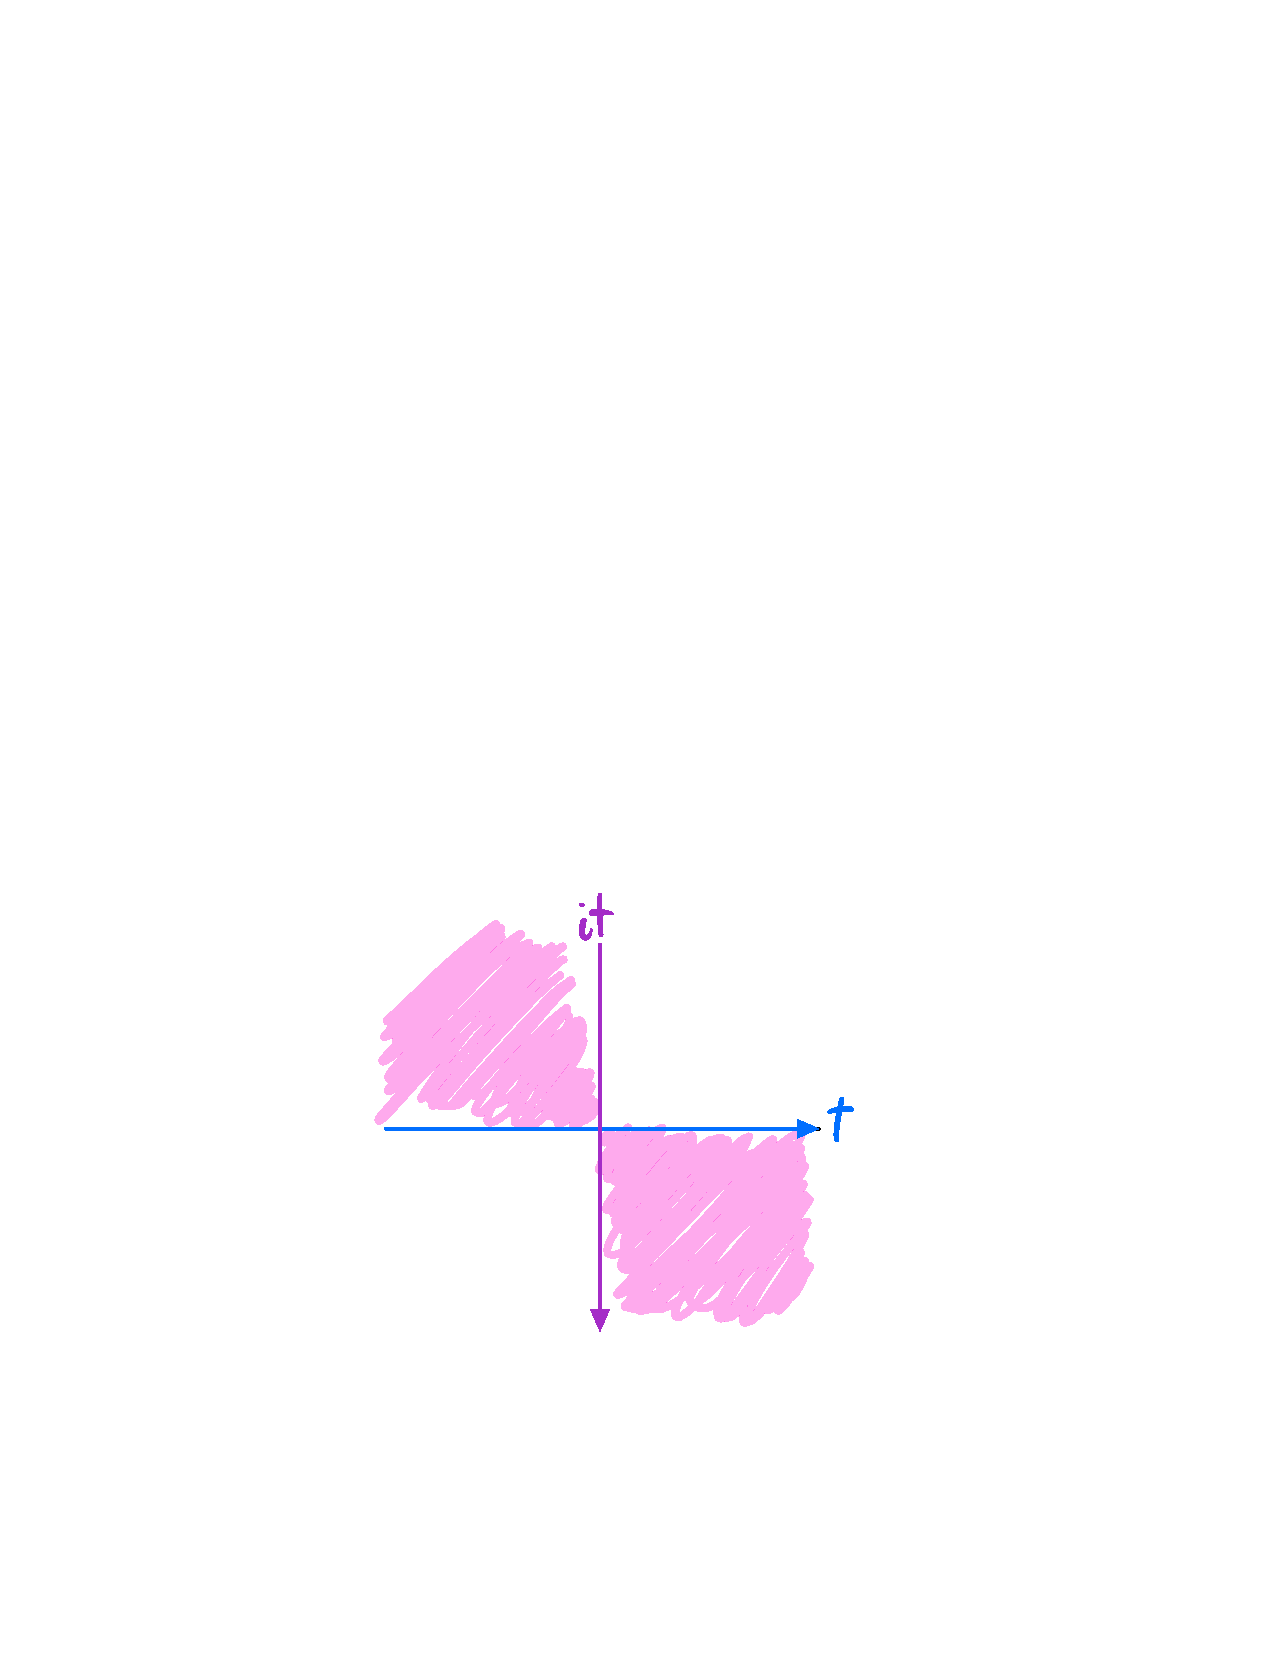
\includegraphics[scale=0.8]{Images/fig-analyticregionwickrotation.pdf}
    \caption{The first term in the above integral is analytic in the fourth quadrant and the second term in the above integral is analytic in the second quadrant. We can then take our contour integral for time which goes along the real axis, and rotate it so it lies on the imaginary axis (Wick rotation). Doing so, our Minkowski space looks Euclidean!}
    \label{fig-analyticregionwickrotation}
\end{figure}



\subsection{Another way to derive the Free-Field Feynman Propagator}
We have derived the two-point function, but not as it appears in most textbooks, or the most useful form for us. We could do it the technical/long way or we can take a pedagogical shortcut. Recall the solution to our QFT solves the field equation:
\begin{equation}
    (-\p^2 + m^2)\varphi(x) = 0
\end{equation}
So what happens if we take this operator and operate it on the time-ordered two-point function? We would find:
\begin{equation}
    (-\p^2 + m^2)\bra{0}J\varphi(x)\varphi(y)\ket{0} = 0.
\end{equation}
Can we just pull this in and get zero? No, not quite; $\p^2$ contains time derivatives, and we have a time ordering of the fields inside the expectation value; we need to take this into account. Let's consider the time derivative:
\begin{equation}
    \dpd{^2}{(x^0)^2}\bra{0}J\varphi(x)\varphi(y)\ket{0}
\end{equation}
and pulling this in and using the product rule and that the derivative of a step function is the dirac delta, as well as the equal time commutation relations:
\begin{equation}
    \begin{split}
        \dpd{^2}{(x^0)^2}\bra{0}J\varphi(x)\varphi(y)\ket{0} &= \dpd{}{x^0}\left(\bra{0}J\dpd{}{x^0}\varphi(x)\varphi(y)\ket{0} + \cancel{\delta(x^0 - y^0)\bra{0}[\varphi(x), \varphi(y)]\ket{0}}\right)
        \\ &= \bra{0}J\dpd{^2\varphi(x)}{(x^0)^2}\varphi(y)\ket{0} + \delta(x^0 - y^0)\bra{0}[\dpd{}{x^0}\varphi(x), \varphi(y)]\ket{0} = -i\delta(x - y)
    \end{split}
\end{equation}
We therefore learn:
\begin{equation}
    (-\p^2 + m^2)\Delta(x, y) = -i\delta(x - y)
\end{equation}
so $\Delta(x, y)$ is a Green's function! Note that this would not be the case for interacting fields as the wave equation is modified. So, we can short circuit all of our work that we have been doing as we can just find a solution to the Green's function equation above. Naively, we can solve this using a Fourier transform so we find:
\begin{equation}
    \Delta(x, y) = \int \frac{d^4k}{(2\pi)^4}e^{ik_\mu(x - y)^\mu} - \frac{i}{k^2 + m^2} 
\end{equation}
where $k^2 = \v{k}^2 - (k^0)^2$. Here the problem becomes apparent; we have a singularity in the above expression. We need to enforce boundary conditions. We take the singularity at $k^0$ and resolve it by adding a small imaginary part into the denominator, in such a way such that when we do the $k^0$ integral (which we could do via Cauchy's integral theorem, if we like):
\begin{equation}
    \Delta(x, y) = \int \frac{d^4k}{(2\pi)^4}e^{ik_\mu(x - y)^\mu} - \frac{i}{k^2 + m^2 - i\e} 
\end{equation}
which fixes the ambiguity and gives us a time-ordered boundary condition. We leave it as an exercise (though it is detailed in the textbook) for how we can write this as something that has two poles, then use partial fractions to separate the two pole terms, and use Cauchy's integral formula to get to:
\begin{equation}
    \Delta(x, y) = \theta(x^0 - y^0) \int \frac{d^3k}{(2\pi)^3 2\omega(\v{k})}e^{i\v{k} \cdot (\v{x} - \v{y}) - i\omega(x^0 - y^0)} + \theta(y^0 - x^0)\int \frac{d^3k}{(2\pi)^3 2\omega(\v{k})}e^{-i\v{k} \cdot (\v{x} - \v{y}) + i\omega(x^0 - y^0)}
\end{equation}
The discussion of analyticity follows exactly as we had before as we have the same expression. There is also a comment we can make about $k^0$. We have poles on the real axis originally, which we add a small $+i\e$ to the denominator to shift them above/below it so we can integrate over the real axis. This enforces boundary conditions. 

We can also consider doing an path integral whose interior does not contain either of the poles (pictured below). Adding it to the integral along the real axis, and taking the boundary to infinity, we get an integral just along the imaginary axis; something that looks Euclidean. This turns out to be extremely useful when we do calculations; we go from a slightly fishy Minkowski space integral to a Euclidean integral that is completely well-defined.

\begin{figure}[htbp]
    \centering
    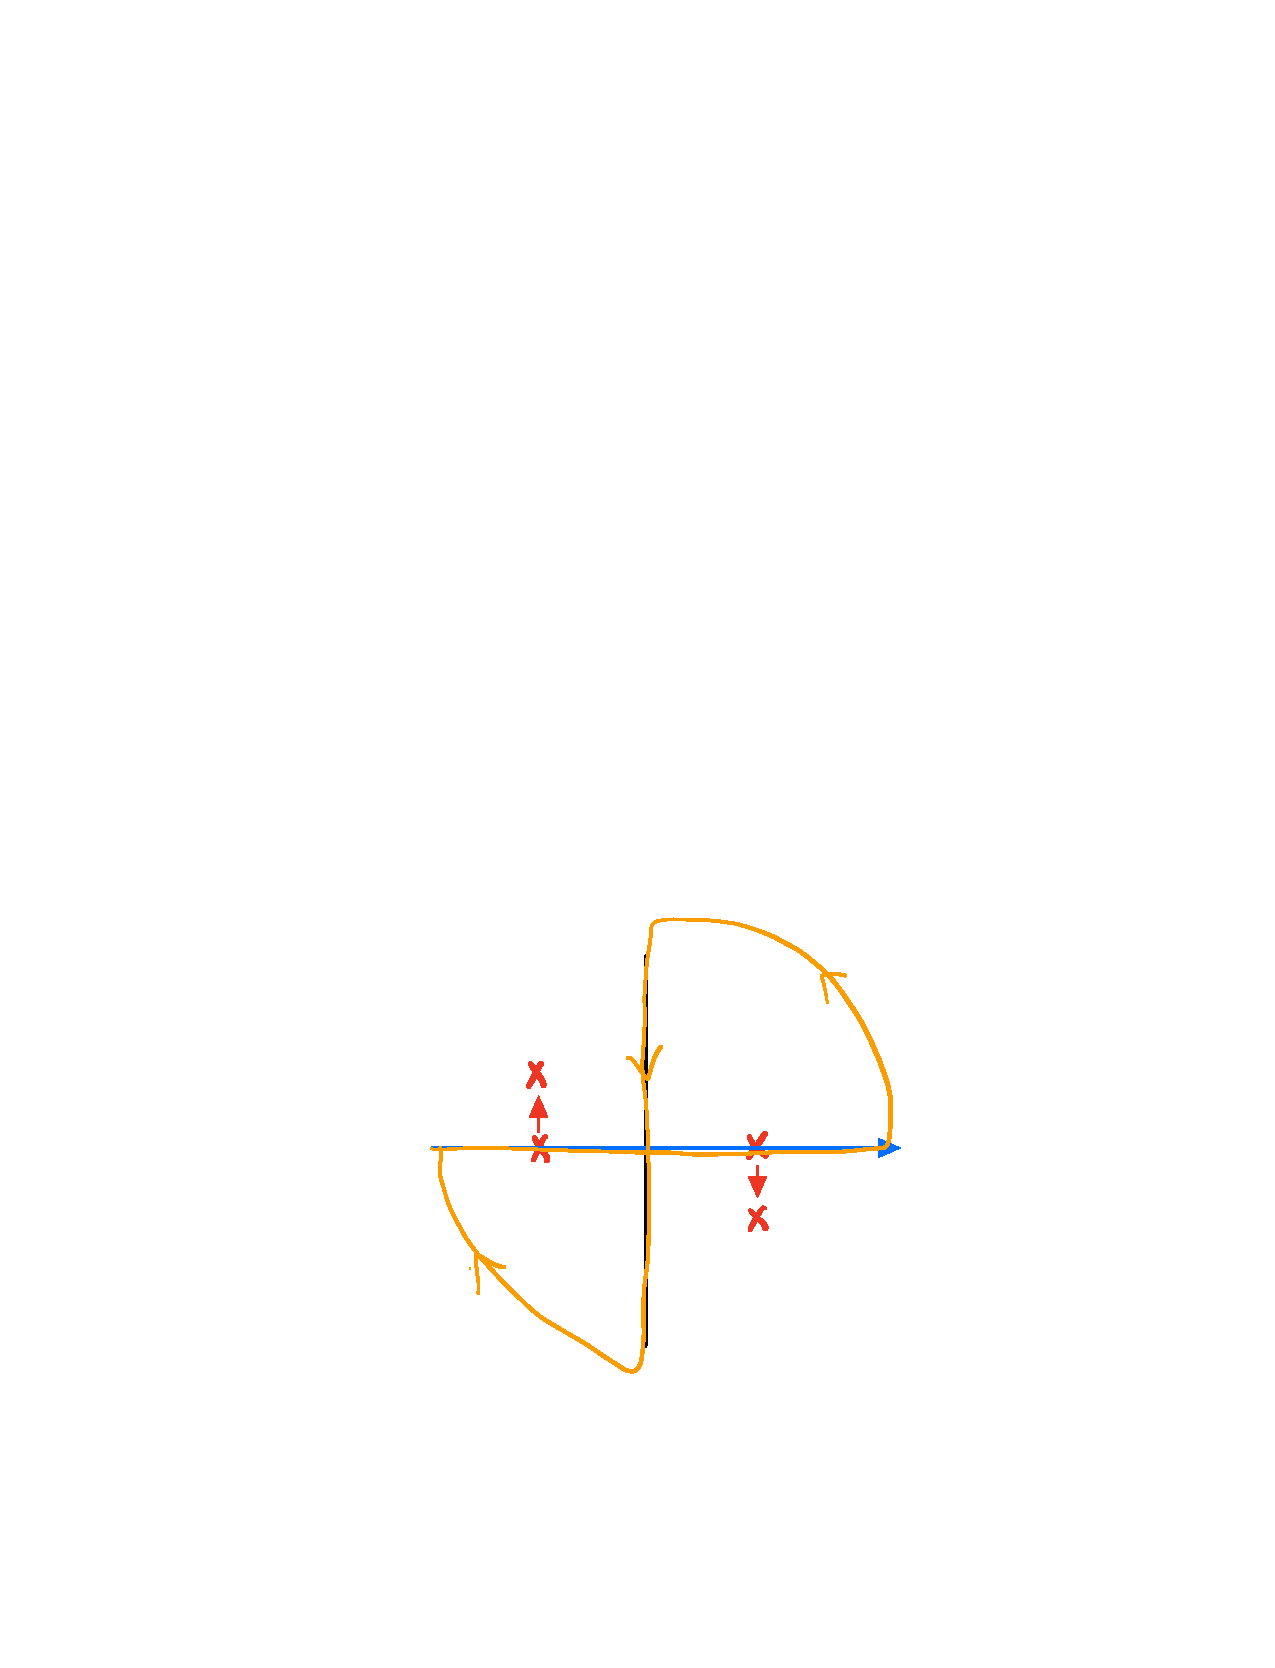
\includegraphics[scale=0.8]{Images/fig-propogatorcontour.pdf}
    \caption{The poles (in red) which originally sat on the time axis have been shifted above/below the real axis via the inclusion of the $-i\e$ in the denominatr of the propogator integral. This allows for a meaningful integral to be taken over the real axis. We can also consider a path integral whose interior contains none of the poles; adding this with the integral over the real axis, we obtain our integral over the imaginary time axis, wherein Minkowski space looks Euclidean.}
    \label{fig-propogatorcontour}
\end{figure}

A few other comments; recall in our discussion of wavepacket dispersion where we added two terms, one for particle and one for antiparticle. This is not the same as the addition of two terms we see here. We were seeing a different kind of Green's function, i.e. a retarded Green's functions (vs. the time-ordered Green's function we see here). This is the appropriate Green's function if we want the past to influence the future. This is a bit of an interesting subtle point; to get causality, we need to do a bit more work compared to what we have done here.

We can use some combinatorics to obtain all other correlation functions; so the free field scalar field theory is completely solved! We will put off studying the interacting field theory until we have a couple more free field theories under our belt. After this in the textbook, we have a chapter about emergent relativistic field theory. It will not be covered in lecture, but it is useful in studying relativistic field theories that go beyond particle physics (e.g. phonons, electrons in graphene). Field theories would be confined to a quite narrow range if we only look at the standard model; the condensed matter side of things offers some interesting cases of study! If we get to the end of the course and have discussed everything else, perhaps we can come back to it.

\subsection{Introduction to the Dirac Field}
There is a basic scalar field amidst the elementary particles - the celebrated Higgs field. The next step up adds spin to the mix (the scalar field has no spin); in particular spin-1/2 as the simplest one. This is the \emph{Dirac Field}, which describes fermions. Since it describes spin, we need another index which at least runs over two. But beyond this, we also need our causality arguments, which requires the existence of an antiparticle. The scalar field did not appear to have this; it did have a negative frequency branch, but this was not a different kind of particle, really. This could happen for dirac-looking field theories as well (though in this case this is not a dirac field, but instead we have majorana particles! which are their own antiparticles). A direct example; electrons and electron holes in the Fermi sea.

The above discussion suggests that we need a 4-component wavefunction (2 spin states for the particle and antiparticle each). This would suggest the guess:
\begin{equation}
    H =? \m{\sqrt{p^2 + m^2} & 0 & 0 & 0 \\ 0 & \sqrt{p^2 + m^2} & 0 & 0 \\ 0 & 0 & -\sqrt{p^2 + m^2} & 0 \\ 0 & 0 & 0 & -\sqrt{p^2 + m^2}}
\end{equation}
but this is ugly, and the spin is basically trivial here; and we don't have a way of knowing that the spin is trivial unless we know things about group theory and representations of the Lorentz group. We would expect that there would be not just two degenerate spin states, as we have here (think relativistic corrections to the hydrogen spectrum!) So the above formula is not correct. Dirac came up with a better idea; can we find some matrices with the correct Hermiticity properties such that the eigenvalues are the same as what we have written above, and it is linear in momentum?
\begin{equation}
    H = i\gv{\alpha}\cdot \nabla + \beta m
\end{equation}
In writing this, Dirac discovered antiparticles; he was however extremely confused with this discovery (even after the experimental discovery of the proton...) It was confusing as it was brilliant. These matrices, in order to have the same spectra, have to be realized as a quaternion factorization of the original guess we had above. They obey the algebra:
\begin{equation}
    \set{\alpha^a, \alpha^b} = 2\delta^{ab}\mathbb{I}, \quad \beta^2 = \mathbb{I}, \quad \set{\alpha^a, \beta} = 0.
\end{equation}
and are Hermitian:
\begin{equation}
    (\alpha^a)^\dag = \alpha^a, \beta^\dag = \beta.
\end{equation}
These are the Dirac Matrices. To study time evolution, we take this Hamiltonian and put it into the Schrodinger equation:
\begin{equation}
    i\dpd{}{t}\psi = (i\gv{\alpha} \cdot \nabla + \beta m)\psi
\end{equation}
where all we have really done is substituted in the Schrodinger operator for the Dirac operator. If we were to derive this theory from the Lagrangian density, we would have something that looks very similar to the original Lagrangian density for our non-relativistic QFT:
\begin{equation}
    \L = i\psi^{\dag}_\sigma \dpd{}{t}\psi_\sigma + \ldots
\end{equation}
with the equal-time anticommutation relations:
\begin{equation}
    \{\psi_a(x), \psi^{\dag}_b(y)\}\delta(x^0 - y^0) = \delta(x - y)
\end{equation}
\begin{equation}
    \{\psi^\dag_a(x), \psi^{\dag}_b(y)\}\delta(x^0 - y^0) = \{\psi_a(x), \psi_b(y)\}\delta(x^0 - y^0) = 0.
\end{equation}

At this point, there is no reason to expect that the states are fermions; one way to figure this out would be that if we had bosons, we would have an unstable theory as we would fill up the negative energy states as much as we want. We need the Pauli principle to stabilize the Fermi sea and ensure that the negative energy states are already filled. Another more formal way to see this; if we use the commutation relations, we would find that the Hamiltonian is not bounded from below. Note that the Poisson bracket actually becomes modified in the case where we have anti-commuting vs. commuting classical fields.

Next time we explore solutions to this theory. Before then; a question; is this theory actually relativistic? We set up the equation such that the spectrum is relativistic with $\sqrt{p^2 + m^2}$. The details we have yet to work out, the answer will (of course) be yes, however.
\newpage
\section{Dirac Field Theory II}
\subsection{The Dirac Equation}
We have been considering the Dirac equation:
\begin{equation}
    i\dpd{}{t}\psi = \left(i\gv{\alpha}\cdot\nabla + \beta m\right)\psi
\end{equation}
where $\alpha^a, \alpha^b, \alpha^c, \beta$ are Hermitian matrices (else the above operator would not be Hermitian) that obey an algebra. 

Why is this the right thing to do? For one, we can see that the above gives the correct dispersion relation (and the cool part - we can do this without even knowing what the matrices are! We only need to know the algebra of commutation relations we obey). How? We consider the square of the above operator, and use that the various terms anticommute. The square of the Hamiltonian has eigenvalues $p^2 + m^2$, so the Hamiltonian itself must have $\pm \set{p^2 + m^2}$. Alright, then how many eigenvalues are there? We can observe that $\alpha^1\alpha^2\alpha^3$ anticommutes with everything, and so when we operate them on the eigenvector of the Hamiltonian, we get another eigenvector but with the opposite sign. Explicitly:
\begin{equation}
    H\psi_\omega = \omega\psi_\omega
\end{equation}
where:
\begin{equation}
    \omega^2 = -\nabla^2 + m^2
\end{equation}
and so:
\begin{equation}
    H\alpha^1\alpha^2\alpha^3\psi_\omega = -\omega\alpha^1\alpha^2\alpha^3\psi_\omega
\end{equation}
In addition, $\alpha^1\alpha^2\alpha^3$ is nonsingular as $(\alpha^1\alpha^2\alpha^3)^{-1} = (\alpha^1\alpha^2\alpha^3)^\dag$. In fact we find that $\alpha^1\alpha^2\alpha^3$ has an equal number (2) of eigenvalues $+1$ and $-1$. So from this we find that there are an equal number of $+\sqrt{p^2 + m^2}$ and $-\sqrt{p^2 + m^2}$ eigenvalues for the Hamiltonian. This discussion is not a big deal, but is meant to show that playing with the algebra is quite profitable - this tells us that any representation of the algebra works. Someday, we may choose an explicit representation to solve the Dirac Equation, but for now let us keep things representation-free and consider space-time symmetry.

\subsection{Space-Time symmetry for the Dirac Field Theory}
Multiplying both sides of the Dirac equation by $i\beta$, we find:
\begin{equation}
    i\left(i\beta\dpd{}{t}\right)\psi = \left(i(i\beta \gv{\alpha})\cdot \nabla + im\right)\psi
\end{equation}
this looks more Lorentz covariant than it did in the previous formula. To emphasize this even further, let us rename $i\beta = \gamma^0$ and $i\beta \alpha^a = \gamma^a$. Since $\beta^2 = 1$ we find that $(\gamma^0)^2 = -1$. We can then rewrite the above equation as:
\begin{equation}\label{eq-diraceq}
    \left(\gamma^\mu \p_\mu + m\right)\psi = 0.
\end{equation}
where:
\begin{equation}
    \set{\gamma^\mu, \gamma^\nu} = 2\eta^{\mu\nu}.
\end{equation}
So the $\gamma$s here compactify the Dirac equation, and their commutation algebra in some sense encodes the algebra of the dirac matrices. We can even more consisely write the above using the Feynman slash notation $\dirac = \gamma^\mu \p_\mu$ to find:
\begin{equation}
    (\dirac + m)\psi = 0.
\end{equation}

So far we have just played with notation; let us now study the symmetries. Recall that the symmetries of the fields we have discussed (scalar, vector, tensor) have symmetries defined by their coordinate transformation properties. So we should do this for the Dirac field. But this is something we have not done yet; spinors don't have a representation as a field. It turns out that the Dirac field transforms like a scalar field - more technically it behaves like a spinor under a sort of ``changing of frames'' (informally phrased here...) but under transformations behaves like a scalar. It it interesting that somehow nature does not take on the simplest possible geometrical features. Already with the very common field describing (e.g.) electrons, the discussion has already become a bit complicated.

So, we have the Dirac field as in Eq. \eqref{eq-diraceq}, and we can study the space-time symmetries. If we just had the field equation, we would consider some infinitesimal transformation of the fields:
\begin{equation}
    \psi \to \psi + \delta \psi
\end{equation}
and this would be a symmetry if:
\begin{equation}
    (\dirac + m)\psi = 0 \implies (\dirac + m)\delta \psi = 0.
\end{equation}
Let's start with translation invariance.

\subsubsection{Translation Invariance}
Translation Invariance would correspond to:
\begin{equation}
    \delta_\mu \psi(x) = -\p_\mu \psi(x).
\end{equation}
Translation of course being generated by a derivative. It is easy to show that this satisfies the symmetry criterion:
\begin{equation}
    0 = \p_\mu \left(0\right) = \p_\mu \left((\dirac + m)\psi\right)\implies (\dirac + m)(\p_\mu \psi) = 0
\end{equation}
So this is shown to be a symmetry. Of course this is not the most useful way, as to apply Noether's theorem to determine the conserved current we require a Lagrangian for the theory. 

\subsubsection{Lorentz Invariance}
A lorentz transformation would correspond to:
\begin{equation}
    \delta \psi = \omega_{\mu\nu}\left(x^\mu \p^\nu - x^\nu \p^\mu\right)\psi + \mathbb{S} \psi
\end{equation}
where we need a matrix $\mathbb{S}$ in order to have the correct transformation. We then have (using the product rule - the $\dirac$ has derivatives!):
\begin{equation}
    (\dirac + m)\delta \psi = \omega_{\mu\nu}(\gamma^\mu \p^\nu - \gamma^\nu \p^\mu)\psi + \omega_{\mu\nu}\left(x^\mu \p^\nu - x^\nu \p^\mu\right)(\dirac + m)\psi + [\gamma^\mu, \mathbb{S}]\p_\mu \psi + \mathbb{S}(\dirac + m)\psi
\end{equation}
From the dirac equation the second term and fourth term vanish, so:
\begin{equation}
    (\dirac + m)\delta \psi = \omega_{\mu\nu}(\gamma^\mu \p^\nu - \gamma^\nu \p^\mu)\psi + [\gamma^\mu, \mathbb{S}]\p_\mu \psi
\end{equation}
The guess for $\mathbb{S}$ is:
\begin{equation}
    \mathbb{S} = -\omega_{\mu\nu}\frac{1}{4}[\gamma^\mu, \gamma^\nu]
\end{equation}
we could get this by process of elimination, considering all of the possible Hermitian matrices in our basis. Let's look at the commutator of $\gamma^\mu$ with $\mathbb{S}$:
\begin{equation}
    \begin{split}
        [\gamma^\mu, \mathbb{S}] &= -\frac{1}{4}\omega_{\rho\sigma}[\gamma^\mu, [\gamma^\rho, \gamma^\sigma]]
        \\ &= -\frac{1}{4}\omega_{\rho\sigma}\left(\gamma^\mu\gamma^\rho\gamma^\sigma - \gamma^\mu \gamma^\sigma \gamma^\rho - \gamma^\rho \gamma^\sigma \gamma^\mu + \gamma^\sigma \gamma^\rho \gamma^\mu\right)
        \\ &= -\frac{1}{4}\omega_{\rho\sigma}\left(\gamma^\mu\gamma^\rho\gamma^\sigma - \gamma^\mu \gamma^\sigma \gamma^\rho - \gamma^\rho \left(2\eta^{\sigma\mu} - \gamma^\mu \gamma^\sigma\right) + \gamma^\sigma \left(2\eta^{\rho\mu} - \gamma^\mu \gamma^\rho\right)\right)
        \\ &= -\frac{1}{4}\omega_{\rho\sigma}\left(\gamma^\mu\gamma^\rho\gamma^\sigma - \gamma^\mu \gamma^\sigma \gamma^\rho + \gamma^\rho \gamma^\mu \gamma^\sigma - \gamma^\rho \gamma^\mu \gamma^\rho - 2\gamma^\sigma \eta^{\sigma\mu} + 2\gamma^\sigma\eta^{\rho\mu}\right)
        \\ &= -\frac{1}{4}\omega_{\rho\sigma}(4)\left(\eta^{\mu\rho}\gamma^\sigma - \eta^{\mu\sigma}\gamma^\rho\right)
        \\ &= \omega_{\rho\sigma}(\gamma^\sigma\p^\rho - \gamma^\rho \p^\sigma)\psi
    \end{split}
\end{equation}
So we conclude:
\begin{equation}
    [\gamma^\mu, \mathbb{S}]\psi = -\omega_{\mu\nu}(\gamma^\mu \p^\nu - \gamma^\nu \p^\mu)\psi
\end{equation}
and therefore:
\begin{equation}
    (\dirac + m)\delta \psi = 0.
\end{equation}
So we have identified a symmetry!
\begin{equation}
    \delta \psi = \left(\omega_{\mu\nu}\left(x^\mu \p^\nu - x^\nu \p^\mu\right)\psi - \omega_{\mu\nu}\frac{1}{4}[\gamma^\mu, \gamma^\nu]\right)\psi
\end{equation}
However, again we don't have a systematic way of identifying the conserved Noether current. We need a Lagrangian density for that. Note that the space and time overlaps in the above (e.g. $[\gamma^0, \gamma^a]$) are Hermitian rather than anti-Hermitian. The boosts are not unitary. And there is a good reason for this; if they were, $\psi^\dag \psi$ would be invariant. But this is density, which is not a Lorentz scalar (it is rather the time component of a current). Lorentz symmetries are not like the usual non-relativistic symmetries where $\psi^\dag \psi$ is invariant, where a symmetry should not change the normalization of the wavefunction.

\subsection{Lagrangian Density for the Noether current}
So - we could try to find a Noether current. In order to do this, let's be pragmatic and find the Lagrangian density for the Dirac field theory (i.e. a Lagrangian density whose variation gives the Dirac equation).

We have the Dirac equation:
\begin{equation}
    (\gamma^\mu \p_\mu + m)\psi(x) = 0.
\end{equation}
so our Lagrangian density should look like:
\begin{equation}
    \begin{split}
        \L &= -i\psi^\dag \gamma^0\gamma^0 \dpd{}{t}\psi - \ldots
        \\ &= -i(\psi^\dag \gamma^0)(\dirac + m)\psi
        \\ &= -i\bar{\psi}(\dirac + m)\psi 
    \end{split}
\end{equation}
where we have defined $\bar{\psi} = \psi^\dag \gamma^0$. We strongly suspect this is Lorentz invariant (at least certainly its critical points are)... Applying Noether's theorem for translations is basically trivial:
\begin{equation}
    \delta\psi = -\p_\mu \psi \implies \delta \L = -\p_\mu \L
\end{equation}
and we can use this to find the conserved Noether's current. The Lorentz transformations takes a little more work, but not too much from our work above:
\begin{equation}
    \begin{split}
        &\delta \psi = \left(\omega_{\mu\nu}\left(x^\mu \p^\nu - x^\nu \p^\mu\right)\psi - \omega_{\mu\nu}\frac{1}{4}[\gamma^\mu, \gamma^\nu]\right)\psi
        \\ \implies & \delta \L = \omega_{\mu\nu}(x^\mu\p^\nu - x^\nu \p^\mu)\L = \p^\mu (-2\omega_{\mu\nu}x^\nu \L)
    \end{split}
\end{equation}
Our question for next time; are we able to write down a stress tensor that we could use for all of these symmetries?
\newpage
\section{Dirac Field Theory III}
We've written down the Lagrangian density for the Dirac field theory:
\begin{equation}
    \L = -i\bar{\psi}(\dirac + m)\psi
\end{equation}
where $\bar{\psi} = \psi^\dag \gamma^0$. We are discussing fermions, so the above Lagrangian concerns anti-commuting classical fields. Last time we discussed the Lorentz invariance of the Dirac Field Theory; now we can use Noether's theorem to find the conserved Noether current.

Before that; a quick question; why do we want a $-i$ there? Because $(\gamma^0)^2 = -1$ and therefore with the $-i$ we get the desired $i\psi^\dag \dpd{}{t}\psi$ term when expanding. It isn't a huge problem if we get the normalization wrong, but we've chosen the canonical normalization here.

Additionally, in the textbook, the derivative has been symmetrized. In the above form, the derivative only acts on the right. In the textbook, there is a $\stackrel{\leftrightarrow}{\dirac} = \stackrel{\rightarrow}{\dirac} - \stackrel{\leftarrow}{\dirac}$ in the Lagrangian due to the symmetrization.

Let's go ahead and analyze the symmetries of this theory. The most important one will not be the space-time translation symmetry, but rather the symmetry under phase transformations.

\subsection{Phase Symmetry}
We consider a variation of the fields:
\begin{equation}
    \delta \psi = i\psi, \quad \delta \bar{\psi} = -i\bar{\psi}
\end{equation}
It is easy to see that the Lagrangian is invariant under this phase transformation:
\begin{equation}
    \L = -i\bar{\psi}(\dirac + m)\psi \mapsto -i(-i\bar{\psi})(\dirac + m)(i\psi) = -i\bar{\psi}(\dirac + m)\psi = \L
\end{equation}
and so $\delta \L = 0$. Noether's theorem tells us that there is a conserved current:
\begin{equation}
    \mathcal{J}^\mu = \delta \psi \dpd{\L}{(\p_\mu \psi)} + \delta \bar{\psi}\dpd{\L}{(\p_\mu \bar{\psi})} = \bar{\psi}\gamma^\mu \psi
\end{equation}
And therefore:
\begin{equation}
    \p_\mu \mathcal{J}^\mu = \p_\mu\left(\bar{\psi}\gamma^\mu \psi\right) = 0.
\end{equation}
Let's give this an overall factor of minus one for notational consistency (so when we have $(\gamma^0)^2 = -1$ the minus sign cancells):
\begin{equation}
    \mathcal{J}^\mu(x) = -\bar{\psi}\gamma^\mu \psi
\end{equation}
and so much like the previous case, we have the conservation of particle number due to phase symmetry.

\subsection{Spacetime Symmetry}
One of these symmetries is just translations:
\begin{equation}
    \delta_{(\mu)}\psi = -\p_\mu \psi
\end{equation}
Then:
\begin{equation}
    \delta_{(\mu)}\L = -\p_\mu \L
\end{equation}
as there is no explicit coordinate dependence in the Lagrangian density. So, this is a symmetry and so we can write:
\begin{equation}
    \mathcal{J}_{(\mu)}^\nu(x) = \delta_{(\mu)}\psi \dpd{\L}{(\p_\nu \psi)} + \delta_{(\mu)} \bar{\psi}\dpd{\L}{(\p_\nu\bar{\psi})} + \eta^{\nu}_\mu \L(x).
\end{equation}
The second term is zero as there is no $\p_\nu \bar{\psi}$ dependence in the Lagrangian density. The first term we can easily read off, so the above evauates to:
\begin{equation}
    \mathcal{J}_{(\mu)}^\nu(x) = -i\bar{\psi}\gamma^\mu \p_\mu \psi - i\eta^{\mu}_\nu \bar{\psi}(\dirac + m)\psi.
\end{equation}
Since we've now derived the conserved current (independent of the equation of motion), we are now free to rewrite it in a cleaner form using the EoM. Doing so, we can eliminate the last term. We can then write the above as:
\begin{equation}
    \mathcal{J}_{(\mu)}^\nu(x) = \mathbb{T}_{0\mu}^{\nu}(x)
\end{equation}
Then:
\begin{equation}
    \p_\nu \mathbb{T}^\nu_{0\mu} = i\bar{\psi}\dirac \p_\mu \psi + i\bar{\psi}\stackrel{\leftarrow}{\dirac}\p_\mu \psi
\end{equation}
The EoM tells us:
\begin{equation}
    (\dirac + m)\psi = 0, \quad \psi^\dag\left(\stackrel{\leftarrow}{\dirac} + m\right) = 0.
\end{equation}
and multiplying on the right by $\gamma^0$:
\begin{equation}
    \bar{\psi}\left(-\stackrel{\leftarrow}{\dirac} + m\right) = 0
\end{equation}
and hence:
\begin{equation}
    \p_\nu \mathbb{T}^\nu_{0\mu} = i\bar{\psi}\dirac \p_\mu \psi + i\bar{\psi}\stackrel{\leftarrow}{\dirac}\p_\mu \psi = 0.
\end{equation}

It's worth pointing out that this stress tensor seems problematic off the bat; it's not symmetric. This turns out to be not a problem, though.

\subsection{Lorentz Symmetry}
The infinitesimal Lorentz transformation of the fields reads:L
\begin{equation}
    \delta \psi = \omega_{\mu\nu}\left((x^\mu \p^\nu - x^\nu \p_\mu)\psi - \frac{1}{4}[\gamma^\mu, \gamma^\nu]\right)\psi
\end{equation}
note that $[\gamma^\mu, \gamma^\nu]$ is often called the spin tensor.

We're going to take a bit of a simplifying shortcut to proceed. We can plug this into the Lagrangian density, and we will find that:
\begin{equation}
    \delta \L = \omega_{\mu\nu}(x^\mu \p^\nu - x^\nu \p^\mu)\L(x)
\end{equation}
which doesn't look like a symmetry, but by the antisymmetry of $\omega$ we can exchange the order of the derivative and hence the above becomes something like $\delta \L = \p(\ldots)$ and so is a symmetry. We find the conserved Noether current to be:
\begin{equation}
    \mathcal{J}^\lambda (x) = (x^\nu \mathbb{T}_0^{\lambda\mu} - x^\mu \mathbb{T}_0^{\lambda \nu})\omega_{\mu\nu} - \frac{i}{4}\bar{\psi}[\gamma^\lambda, [\gamma^\mu, \gamma^\nu]]\psi \omega_{\mu\nu}.
\end{equation}
We then have:
\begin{equation}
    0 = \p_\lambda \mathcal{J}^\lambda = (\mathbb{T}_0^{\nu\mu} - \mathbb{T}_0^{\mu\nu})\omega_{\mu\nu} + \omega_{\mu\nu}\p_\lambda\left(\frac{i}{4}\bar{\psi}[\gamma^\lambda, [\gamma^\mu, \gamma^\nu]]\psi\right)
\end{equation}
the above identity could be proven using algebra, but let's just rely on Noether's theorem to save us the Hassle. However, the above identity does give us something nice; it allows us to improve the stress tensor, symmetrizing it:
\begin{equation}
    \mathbb{T}^{\mu\nu}(x) = \frac{i}{2}\bar{\psi}\left(\gamma^\mu \p^\nu + \gamma^\nu \p^\mu\right)\psi
\end{equation}
%Note the bracket $[\gamma^\lambda, [\gamma^\mu, \gamma^\nu]]$ is antisymmetric in the indices and hence taking further derivatives will result in zero
If we contract the above with a Killing vector, we find:
\begin{equation}
    \mathcal{J}^{\lambda}_f = \mathbb{T}^{\mu\nu}\hat{f}_\nu(x).
\end{equation}
What is more, if the fermion is massless, the $\mathbb{T}^{\mu\nu}$ has vanishing trace! This is because when we take the trace, $\gamma^\mu\p^\nu$ turns into a $\dirac$. Therefore $\mathbb{T}^{\mu\nu}\hat{f}_\nu(x)$ is a conserved current even if $\hat{f}$ is not a Killing vector but a conformal Killing vector.

If we look at the Hamiltonian here, we get the (matrix-valued) Dirac Hamiltonian which we have to confirm is actually sensible. This will have negative and positive eigenvalues. If we chose bosons instead of fermions, it would not be bounded from below; as bosons will arbitrarily fill the negative energy states. We have the so called ``Dirac sea'', which is stabilized in the case of Fermions (as it is totally filled), like the case of the Fermi sea. Note that in constrast to the Fermi sea however, we have an infinitely deep sea! Another contrast; in the Fermi gas system we have a metal, while in the Dirac field system we have an insulator as there is an energy gap between the dirac sea (negative energy states) and the positive energy states.

\begin{figure}[htbp]
    \centering
    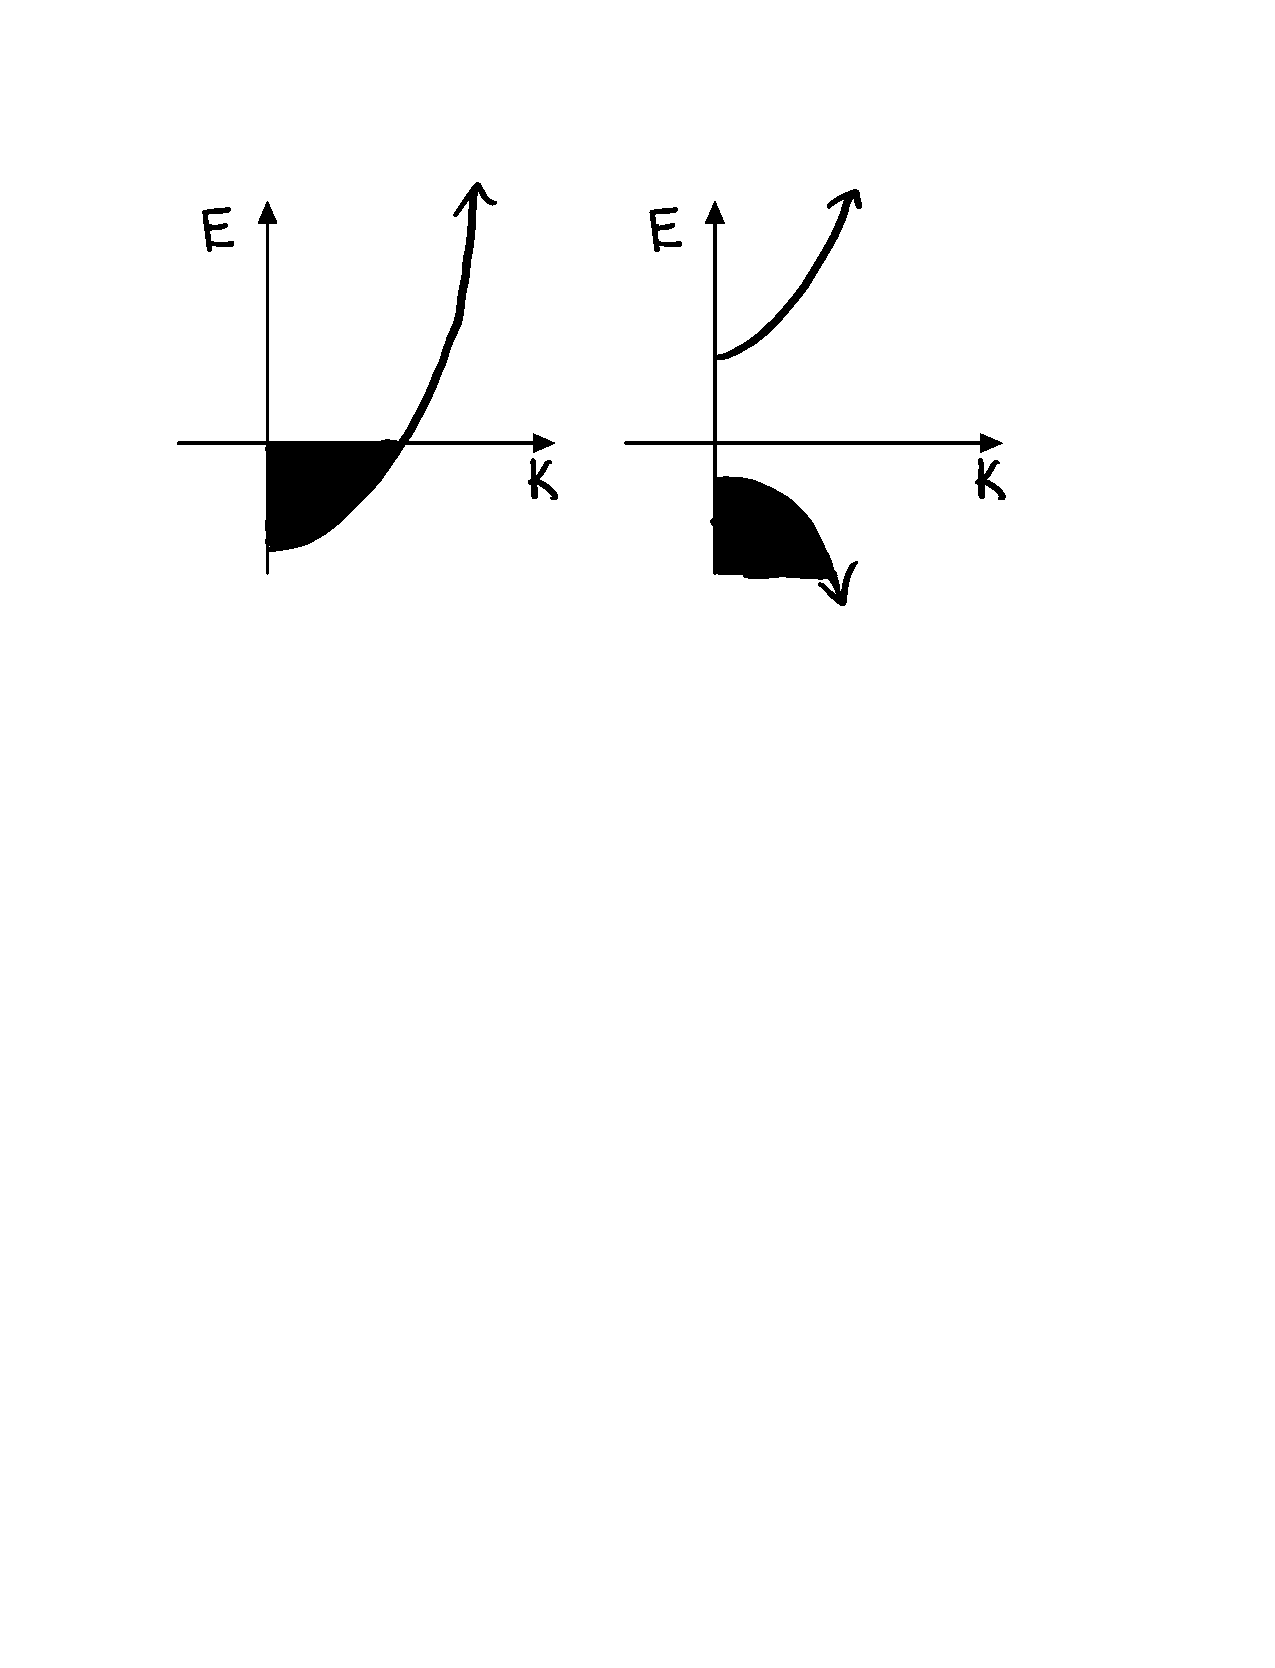
\includegraphics[scale=0.7]{Images/fig-fermidiracseas.pdf}
    \caption{Sketch of the energies of a degenerate Fermi gas (left) and the Dirac field (right). The shaded region corresponds to the Fermi and Dirac ``seas'', respectively.}
    \label{fig-fermidiracseas}
\end{figure}

The infinitely deep quality of the Dirac sea has some interesting implications. It gives us a way to violate some symmetries, for example, e.g. the symmetry that shifts all levels by a unit. In the dirac sea case, if we moved up one unit we would create a particle in the positive energy region and if we moved down unit we would create a hole in the negative energy region.


\subsection{Starting to Solve the Dirac Equation}
So, we've pretty comprehensively studied the symmetries of the Dirac theory. The last thing left is to actually solve it. We consider the representation:
\begin{equation}
    \gamma^0 = \m{0 & \mathbb{I} \\ -\mathbb{I} & 0}, \quad \gamma^a = \m{0 & \sigma^a \\ \sigma^a & 0}
\end{equation}
where $\sigma^a$ are the Pauli matrices:
\begin{equation}
    \sigma^1 = \paulix, \quad \sigma^2 = \pauliy, \quad \sigma^3 = \pauliz
\end{equation}
We then have that rotations in the $ab$ plane (about the $c$ axis) looks like:
\begin{equation}
    \frac{i}{4}[\gamma^a, \gamma^b] = -\e^{abc}\m{\frac{\sigma^c}{2} & 0 \\ 0 & \frac{\sigma^c}{2}}
\end{equation}
where the commutators are easily computed using the Pauli algebra. This is a nice representation as the spins are indeed actual spins/rotations, in a sense. 

We consider a four-spinor plane wave ansatz:
\begin{equation}
    \psi(x) = \m{u \\ v}e^{i\left(\v{k}\cdot\v{x} - \omega(\v{k})t\right)}
\end{equation}
In the chosen matrix representation, the Dirac equation with the above ansatz becomes:
\begin{equation}
    \m{m & i\omega + i\gv{\sigma} \cdot \v{k} \\ -i\omega + i\gv{\sigma} \cdot \v{k} & m}\m{u\\v} = 0.
\end{equation}
and so if we solve the eigenvalues and eigenvectors of the above, we are done! We can see that the spin plays a very active role here due to the $\gv{\sigma}\cdot \v{k}$ (spin-momentum coupling). We can see that spin is not a good quantum number here as the spin rotation messes it up. What is a good quantum number is if we look for the eigenvalues of $\gv{\sigma} \cdot \v{k}$ - this is related to the spin along the direction of motion of the particle, or the \emph{helicity}. We will discuss it more next time, where we will conclude our discussion of the Dirac field. We will then move onto photons!
\newpage
\section{Dirac Theory IV, Photon Field I}
To finish up our discussion of the Dirac field, we discuss its solutions. We then move onto the photon field. One thing we notice as we get to more realistic fields is that they get more complicated. We started by looking at the scalar field, which corresponds to the Higgs field (and some other emergent fields). The more realistic field is the Dirac field, which describes electrons and other spin-1/2 massive particles. The quantization is only a tiny bit more complicated than it was with the scalar field. The next level up is gravity, or Yang-Mills, which have the same sort of complications, but more complicated.


\subsection{Solving the Dirac Equation}
We wish to solve the Dirac equation:
\begin{equation}
    (\dirac + m)\psi(x) = 0.
\end{equation}
in other words, find the kernel of the $\dirac + m$ operator. We notice there are no $x$s or $t$s in the expression, so it is automatic what we have to do; make a plane wave ansatz!
\begin{equation}
    \psi(x) = \psi_ke^{ik^\mu x_\mu} = \m{u(k) \\ v(k)}e^{i\v{k} \cdot \v{x} - i\omega(\v{k}) t}
\end{equation}
This is part of it. The other part is we need to know what the $\gamma^\mu$ matrices are; it is easier to solve the equation if we choose an explicit representation. We choose the representation:
\begin{equation}
    \gamma^0 = \m{0 & \mathbb{I} \\ -\mathbb{I} & 0}, \quad \gamma^a = \m{0 & \sigma^a \\ \sigma^a & 0}
\end{equation}
With this ansatz and choice of representation, the dirac equation becomes:
\begin{equation}
    \m{m & -i\omega + i\gv{\sigma} \cdot \v{k} \\ i\omega + i\gv{\sigma} \cdot \v{k} & m} \m{u \\ v} = 0.
\end{equation}
where if there is just a number, there is implicitly a 2x2 identity matrix. We have to solve the above; this is easy! The only complications are with the $\gv{\sigma} \cdot \v{k}$; we will to this end look for $u, v$ that are eigenvectors of this:
\begin{equation}
    \gv{\sigma} \cdot \v{k} v_\lambda = \lambda v_\lambda
\end{equation}
And this will have the very nice effect of reducing the matrix we are diagonalizing into a matrix of only numbers. Solving for the eigenvalues is very easy; notice:
\begin{equation}
    (\gv{\sigma} \cdot \v{k})^2 = k^ak^b \sigma^a\sigma^b = \frac{1}{2}k^ak^b \{\sigma^a, \sigma^b\} = \frac{1}{2}k^ak^b 2\delta_{ab} =  \v{k}^2
\end{equation}
and so:
\begin{equation}
    \lambda^2 = \v{k}^2 \implies \lambda = \pm \abs{\v{k}}
\end{equation}
How do we figure out if they are plus or minus? Well of course $\Tr(\sigma^a) = 0$ and so the eigenvalues must sum to zero, so there is one $+\abs{\v{k}}$ eigenvalue and one $-\abs{\v{k}}$ eigenvalues. So:
\begin{equation}
    \gv{\sigma} \cdot \v{k} v_s = s\abs{\v{k}}v_s, \quad s = \begin{cases}
        +1 \\ -1
    \end{cases}
\end{equation}
So we can plug this back into our matrix equation; since the matrix mixes $u, v$ we can write them with the same eigenvalue:
\begin{equation}
    \m{m & -i\omega + is\abs{\v{k}} \\ i\omega + is\abs{\v{k}} & m}\m{u_s \\ v_s} = 0.
\end{equation}
for this to have a solution, we have to have a non-empty kernel, i.e. the determinant must vanish, so writing down the determinant of the above:
\begin{equation}
    m^2 - (\omega^2 - s^2\v{k}^2) = 0
\end{equation}
with $s^2 = 1$, we easily find the frequency to be:
\begin{equation}
    \omega = \pm \sqrt{\v{k}^2 + m^2}
\end{equation}
From this we can find a relation between the spinors $u_s, v_s$:
\begin{equation}
    i(\omega + s\abs{\v{k}})u_s + mv_s = 0
\end{equation}
which then we obtain:
\begin{equation}
    v_s = -i\frac{\omega + s\abs{\v{k}}}{m}u_s
\end{equation}
we may want to normalize the spinors:
\begin{equation}
    \abs{u_s}^2 + \abs{v_s}^2 = 1
\end{equation}
and so:
\begin{equation}
    \abs{u_s}^2 + \left(\frac{\omega + s\abs{\v{k}}}{m}\right)^2 \abs{u_s}^2 = 1
\end{equation}
Therefore:
\begin{equation}
    \frac{m^2 + \v{k}^2 + \omega^2 + 2s\omega\abs{\v{k}}}{m^2}\abs{u_s}^2 = 1
\end{equation}
And since the first two terms in the above add up to $\omega^2$, we find:
\begin{equation}
    \frac{2\omega(\omega + s\abs{\v{k}})}{m}\abs{u_s}^2 = 1
\end{equation}
and so:
\begin{equation}
    u_s = \frac{m}{\sqrt{2\omega(\omega + s\abs{\v{k}})}}\hat{u}_s
\end{equation}
where is a spinor which satisfies:
\begin{equation}
    \gv{\sigma} \cdot \v{k} \hat{u}_s = s\abs{\v{k}}\hat{u}_s
\end{equation}
\begin{equation}
    \hat{u}_s^\dag \hat{u}_s = 1.
\end{equation}

Let us review; we have found four solutions; we have the defining equation for $\hat{u}_s$ which gives us two solutions 
(one for $s = \pm 1$) and then we get two solutions each when plugging into the equation for $u_s$ (as we have $\omega = \pm \sqrt{\v{k}^2 + m^2}$) which determines $v_s$. This makes sense with our expectation that a four-by-four matrix equation should have four solutions!

So, we have the solutions to the Dirac equation:
\begin{equation}
    \psi_{s\omega} = \m{u_{s\omega} \\ v_{s\omega}}
\end{equation}
with:
\begin{equation}
    \psi^\dag_{s\omega}\psi_{s\omega} = 1.
\end{equation}

The most general solution would be a superposition (over $\v{k}, \omega, s$), so:
\begin{equation}
    \psi(x) = \int \frac{d^3k}{(2\pi)^{3/2}}\left[e^{i\v{k} \cdot \v{x} - i\sqrt{\v{k}^2 + m}t}\sum_s \m{u_{s\omega}(\v{k}) \\ v_{s\omega}(\v{k})}a_s(\v{k}) + e^{-i\v{k} \cdot \v{x} + i\sqrt{\v{k}^2 + m^2}t}\sum_s \m{u_{s-\omega}(\v{k}) \\ v_{s-\omega}(\v{k})} b_s^\dag(\v{k}) \right]
\end{equation}
note that we don't have all the junk we did in the scalar field case, as here our objects are more akin to non-relativistic fermions, which only had the plane wave normalization. $s$ is known as the Helicity. It is not its spin projection along some fixed axis, but rather the projection of spin along its motion (which is some axis, but not a fixed one; it can change as it moves around). To get the equal time commutation realtions for the field $\psi$, we enforce:
\begin{equation}
    \{a_s(\v{k}), a^\dag_{s'}(\v{l})\} = \delta_{ss'}\delta^3(\v{k} - \v{l})
\end{equation}
\begin{equation}
    \{b_s(\v{k}), b^\dag_{s'}(\v{l})\} = \delta_{ss'}\delta^3(\v{k} - \v{l})
\end{equation}
(and all other combinations that we do note write are zero). which implies:
\begin{equation}
    \{\psi_a(\v{x}), \psi_b^\dag(\v{y})\}\delta(x^0 - y^0) = \delta_{ab}\delta^4(x - y)
\end{equation}
so in some sense we have solved our quantum field theory! We can proceed to create our Hilbert (more accurately, Fock) space. We have our vacuum state $\ket{\mathcal{O}}$, which corresponds to the state with all the negative energy states (in the Dirac sea) filled and all of the positive energy ones empty. This is normalized:
\begin{equation}
    \braket{\mathcal{O}}{\mathcal{O}} = 1
\end{equation}
and such that it is annihilated by the particle/hole annihilation operators:
\begin{equation}
    a_s(\v{k})\ket{\mathcal{O}} = 0, \quad b_s(\v{k})\ket{\mathcal{O}} = 0
\end{equation}
and we have the basis states:
\begin{equation}
    \ket{\mathcal{O}}, a_s^\dag(\v{k})\ket{\mathcal{O}}, b_s^\dag(\v{k})\ket{\mathcal{O}}, a_{s_1}^\dag(\v{k}_1)a_{s_2}^\dag(\v{k}_2)\ket{\mathcal{O}}, \ldots
\end{equation}
We can integrate the $\mathbb{T}^{tt}$ component of the stress tensor to get the Hamiltonian:
\begin{equation}
    H = \int d^3 \mathbb{T}^{00} = \sum_s \int d^3k \sqrt{k^2 + m^2}\left(a_s^\dag(\v{k})a_s(\v{k}) + b_s^\dag(\v{k})b_s(\v{k})\right)
\end{equation}
and we can see these are just the number operators times the energies of the particles/holes (anti-particles) they are counting. This is a stable system. If we had made the mistake of considering this system as bosonic, what would have happened? We would replace the anti-commutators with commutators, and it would follow from our Lagrangian density. We could have gone down what turns out to be the wrong path, and everything would be fine up to the construction of the Fock space (we would have more space because no exclusion principle), but anyway. But something goes wrong when we look at the Hamiltonian. If we had bosons instead of fermions, we would have:
\begin{equation}
    H = \int d^3 \mathbb{T}^{00} = \sum_s \int d^3k \sqrt{k^2 + m^2}\left(a_s^\dag(\v{k})a_s(\v{k}) - b_s^\dag(\v{k})b_s(\v{k})\right)
\end{equation}
this is terrible! The Hamiltonian is not bounded from below. By exciting the $b$s, we can get an arbitrarily low energy. This would be ok for a free field theory, but as soon as we try to apply it to something in the real world (which couples it to things), we would get transitions, which pushes the system to lower energy states, making it highly unstable. This construction only makes sense if the fields are fermions. It is not a stable theory if we have bosons. This is part of a bigger theorem known as the spin-statistics theorem (a complicated spinoff of our discussion about analyticity). This can be proved that a Lorentz invariant theory has a spin-statistics theorem. It has to do with the fact that if you have a half integer spin, the field is double valued; (spinors have $R_n(2\pi) = -1$, $R_n(4\pi) = 1$), and combining this with lorentz invariance yields the spin-statistics theorem.

By the way, if we calculate the number operators:
\begin{equation}
    \mathcal{N} = \int d^3x \psi^\dag(x)\psi(x) = \sum_s \int d^3k (a_s^\dag(\v{k})a_s(\v{k}) - b_s^\dag(\v{k})b_s(\v{k}))
\end{equation}
This makes the number operators very suitable for describing electric charge; the $a$s create electrons, $b$s create positrons.

\subsection{The Photon Field and Maxwell's Equations}
We now proceed to study the quantum field theory for the photons. This will be a weakly coupled bosonic theory. Recall from our initial discussion about bosonic fields that Bose fields act somewhat classically. We can proceed to get the Lagrangian from this, and we get something that we are intimately familiar with; classical electrodynamics! So, we can carry these equations of motion over and use them to study the theory of quantum electrodynamics. This might be suspect; how might we know that there aren't terms proportional to $\frac{1}{\hbar}$ etc.? In some sense we don't know, but being a QFT there are certain conditions that need to be mathematically satisfied. These constraints tell us that we don't need to correct Maxwell's equations.

This isn't to say that there aren't effective field theories, which (e.g.) can be used to study photon-photon scattering (a rare event) which looks like something beyond classical electrodynamics (as classical waves do not scatter off of each other) but this is understood as a quantum process, where the photons disintegrate into ``virtual'' electrons and positrons which scatter from each other and reannhilate etc.

In any case, we have a pretty good guess for how to start with talking about photons; just write down maxwell's equations! In nonrelativistic notation, they are written in any classical electrodynamics textbook. But they are much more consisely written in relativistic notation. We consider the electromagnetic tensor $\mathcal{F}^{\mu\nu}$ with $\mathcal{F}^{0a} \sim E^a$ and $\mathcal{F}^{ab} \sim \e^{abc}B^c$. We can then forget about how Lorentz transforms work, and just use that $\mathcal{F}^{\mu\nu}$ transforms like a tensor! When we stick the electromagnetic fields into $F^{\mu\nu}$, the Maxwell equations are simple to write (we have two sets):
\begin{equation}
    \p_\mu \mathcal{F}^{\mu\nu}(x) = -\mathcal{J}^\nu(x)
\end{equation}
\begin{equation}
    \p_\mu \mathcal{F}_{\nu\lambda}(x) + \p_\nu \mathcal{F}_{\lambda \mu}(x) + \p_\lambda \mathcal{F}_{\mu\nu}(x) = 0.
\end{equation}
What is normally done to proceed from here is to write down a solution to the above equation. This might be familiar as a Bianchi identity. The equation tells us that it is closed, and on simple spaces this tells us it is exact, and so a solution of this is written as:
\begin{equation}
    \mathcal{F}_{\mu\nu}(x) = \p_\mu A_\nu - \p_\nu A_\mu
\end{equation}
i.e. in terms of a four-vector field $A_\mu$. Given some topology and boundary considerations, this is a unique solution. After determining this, we can take $A_\mu$ to be the dynamical variable, and then use the first set of Maxwell equations to determine how it is governed. At the classical level, $A_\mu$ is not particularly important 

\end{document}